%----------------------------------------------------------------------------------------
%	PACKAGES AND OTHER DOCUMENT CONFIGURATIONS
%----------------------------------------------------------------------------------------

\documentclass[
11pt, % The default document font size, options: 10pt, 11pt, 12pt
%oneside, % Two side (alternating margins) for binding by default, uncomment to switch to one side
english, % ngerman for German
singlespacing, % Single line spacing, alternatives: onehalfspacing or doublespacing
%draft, % Uncomment to enable draft mode (no pictures, no links, overfull hboxes indicated)
%nolistspacing, % If the document is onehalfspacing or doublespacing, uncomment this to set spacing in lists to single
%liststotoc, % Uncomment to add the list of figures/tables/etc to the table of contents
%toctotoc, % Uncomment to add the main table of contents to the table of contents
%parskip, % Uncomment to add space between paragraphs
%nohyperref, % Uncomment to not load the hyperref package
headsepline, % Uncomment to get a line under the header
%chapterinoneline, % Uncomment to place the chapter title next to the number on one line
%consistentlayout, % Uncomment to change the layout of the declaration, abstract and acknowledgements pages to match the default layout
]{MastersDoctoralThesis} % The class file specifying the document structure

\usepackage[utf8]{inputenc} % Required for inputting international characters
\usepackage[T1]{fontenc}

%\usepackage{mathpazo} % Use the Palatino font by default
% needs to be turned off for cyrilic

%Russian-specific packages
%--------------------------------------
\usepackage[T2A]{fontenc}
\usepackage[utf8]{inputenc}
\usepackage[russian]{babel}

%\usepackage[backend=bibtex,style=authoryear,natbib=true]{biblatex} % Use the bibtex backend with the authoryear citation style (which resembles APA)

% chicago style but with comma 
\usepackage[style=chicago-authordate,strict,backend=bibtex8, maxcitenames=2, maxbibnames=999%
babel=other,bibencoding=inputenc]{biblatex}
\renewcommand*{\nameyeardelim}{\addcomma\space}

\addbibresource{openbiodiv.bib} % The filename of the bibliography

% long citations

\makeatletter
\newcommand{\tempmaxup}[1]{\def\blx@maxcitenames{\blx@maxbibnames}#1}
\makeatother

\DeclareCiteCommand{\longfullcite}[\tempmaxup]
  {\usebibmacro{prenote}}
  {\usedriver
     {\DeclareNameAlias{sortname}{default}}
     {\thefield{entrytype}}}
  {\multicitedelim}
  {\usebibmacro{postnote}}

\usepackage[autostyle=true]{csquotes} % Required to generate language-dependent quotes in the bibliography

%code listings
\usepackage{listings}
\usepackage{soul} % for underline

\usepackage{algorithm}
\usepackage{algpseudocode}

\lstdefinestyle{customr}{
  belowcaptionskip=1\baselineskip,
  breaklines=true,
 % frame=L,
  xleftmargin=\parindent,
  language=R,
  showstringspaces=false,
  basicstyle=\footnotesize\ttfamily,
  keywordstyle=\bfseries\color{black!40!black},
  commentstyle=\itshape\color{purple!40!black},
  identifierstyle=\color{black},
  stringstyle=\color{black},
}

\lstdefinestyle{customsparql}{
  belowcaptionskip=1\baselineskip,
  breaklines=true,
 % frame=L,
  xleftmargin=\parindent,
  language=SPARQL,
  showstringspaces=false,
  basicstyle=\footnotesize\ttfamily,
  keywordstyle=\bfseries\color{black!40!black},
  commentstyle=\itshape\color{purple!40!black},
  identifierstyle=\color{black},
  stringstyle=\color{black},
}


\newcommand\cl{\lstinline[style=customr]}

\def\todo#1{\medskip\par\noindent\textcolor{red}{\bf TODO: #1}\par\medskip}
\def\KIRIL#1{\medskip\par\noindent\textcolor{red}{\bf KIRIL: #1}\par\medskip}
\def\LYUBO#1{\medskip\par\noindent\textcolor{red}{\bf LYUBO: #1}\par\medskip}

%----------------------------------------------------------------------------------------
%	MARGIN SETTINGS
%----------------------------------------------------------------------------------------

\geometry{
	paper=a4paper, % Change to letterpaper for US letter
	inner=2.5cm, % Inner margin
	outer=3.8cm, % Outer margin
	bindingoffset=.5cm, % Binding offset
	top=1.5cm, % Top margin
	bottom=1.5cm, % Bottom margin
	%showframe, % Uncomment to show how the type block is set on the page
}


%----------------------------------------------------------------------------------------
%	THESIS INFORMATION
%----------------------------------------------------------------------------------------
\thesistitle{OpenBiodiv: отворена система за управление на данни за биологичното разнообразие} % Your thesis title, this is used in the title and abstract, print it elsewhere with \ttitle
\supervisor{проф. д-р Любомир \textsc{Пенев}} % Your supervisor's name, this is used in the title page, print it elsewhere with \supname
\consultant{доц. д-р Кирил \textsc{Симов}}

\examiner{} % Your examiner's name, this is not currently used anywhere in the template, print it elsewhere with \examname
\degree{``доктор''} % Your degree name, this is used in the title page and abstract, print it elsewhere with \degreename
\degreeprogram{``Информатика'' (01.01.2012 г.)}
\profession{4.6 ``Информатика и компютърни науки''}
\author{Виктор \textsc{Сендеров}} % Your name, this is used in the title page and abstract, print it elsewhere with \authorname
\addresses{} % Your address, this is not currently used anywhere in the template, print it elsewhere with \addressname

\subject{Biological Sciences} % Your subject area, this is not currently used anywhere in the template, print it elsewhere with \subjectname
\keywords{} % Keywords for your thesis, this is not currently used anywhere in the template, print it elsewhere with \keywordnames
\university{\href{http://www.bas.bg}{Българска академия на науките}}
\company{\href{http://pensoft.net}{Академично издателство "Пенсофт"}}

% Your university's name and URL, this is used in the title page and abstract, print it elsewhere with \univname
\department{\href{http://www.iict.bas.bg}{Институт по
информационни и комуникационни технологии }} % Your department's name and URL, this is used in the title page and abstract, print it elsewhere with \deptname
\group{\href{http://http://lml.bas.bg/}{Лингвистично моделиране и обработка на знания}} % Your research group's name and URL, this is used in the title page, print it elsewhere with \groupname



\AtBeginDocument{
\hypersetup{pdftitle=\ttitle} % Set the PDF's title to your title
\hypersetup{pdfauthor=\authorname} % Set the PDF's author to your name
\hypersetup{pdfkeywords=\keywordnames} % Set the PDF's keywords to your keywords
}

\begin{document}

\frontmatter % Use roman page numbering style (i, ii, iii, iv...) for the pre-content pages

\pagestyle{plain} % Default to the plain heading style until the thesis style is called for the body content

%----------------------------------------------------------------------------------------
%	TITLE PAGE
%----------------------------------------------------------------------------------------

\begin{titlepage}
\begin{center}
\vspace*{.06\textheight}
{\scshape\LARGE \univname\par}\vspace{1.5cm} % University name
{\scshape\LARGE \compname\par}\vspace{1.5cm} % University name
\textsc{\Large АВТОРЕФЕРАТ}\\[0.5cm] % Thesis type

\HRule \\[0.4cm] % Horizontal line
{\huge \bfseries \ttitle\par}\vspace{0.4cm} % Thesis title
\HRule \\[1.5cm] % Horizontal line
 
\begin{minipage}[t]{0.4\textwidth}
\begin{flushleft} \large
\emph{Автор:}\\
\href{http://senderov.net}{\authorname} % Author name - remove the \href bracket to remove the link
\end{flushleft}
\end{minipage}
\begin{minipage}[t]{0.4\textwidth}
\begin{flushright} \large
\emph{Научен ръководител:} \\
\href{http://pensoft.net}{\supname} \\ % Supervisor name - remove the \href bracket to remove the link  
\emph{Научен консултант:} \\
\href{http://bultreebank.org/en/our-team/kiril-simov/}{\consname} % Supervisor name - remove the \href bracket to remove the link  

\end{flushright}
\end{minipage}\\[3cm]

% TODO Ask Kiril about научна област, научна специалност от заглавната страница на автореферата
\large 
\textit{За придобиване на образователната и научна степен \degreename\\
по докторска програма \degreeprogramname\\
професионално направление \professionname}\\[0.3cm] % University requirement text

\vfill

%{\large \today}\\[4cm] % Date
%\includegraphics{Logo} % University/department logo - uncomment to place it
 
\vfill
\end{center}
\end{titlepage}

%----------------------------------------------------------------------------------------
%	DECLARATION PAGE
%----------------------------------------------------------------------------------------

% \begin{declaration}
% \addchaptertocentry{\authorshipname} % Add the declaration to the table of contents
% \noindent I, \authorname, declare that this thesis titled, \enquote{\ttitle} and the work presented in it are my own. I confirm that:

% \begin{itemize} 
% \item This work was done wholly or mainly while in candidature for a research degree at this University.
% \item Where any part of this thesis has previously been submitted for a degree or any other qualification at this University or any other institution, this has been clearly stated.
% \item Where I have consulted the published work of others, this is always clearly attributed.
% \item Where I have quoted from the work of others, the source is always given. With the exception of such quotations, this thesis is entirely my own work.
% \item I have acknowledged all main sources of help.
% \item Where the thesis is based on work done by myself jointly with others, I have made clear exactly what was done by others and what I have contributed myself.\\
% \end{itemize}
 
% \noindent Signed:\\
% \rule[0.5em]{25em}{0.5pt} % This prints a line for the signature
 
% \noindent Date:\\
% \rule[0.5em]{25em}{0.5pt} % This prints a line to write the date
% \end{declaration}

% \cleardoublepage




\mainmatter % Begin numeric (1,2,3...) page numbering

\pagestyle{thesis} % Return the page headers back to the "thesis" style

% Chapter 1
\addchap{Въведение}
\label{chapter-introduction} 
%----------------------------------------------------------------------------------------
% Define some commands to keep the formatting separated from the content 
\newcommand{\keyword}[1]{\textbf{#1}}
\newcommand{\tabhead}[1]{\textbf{#1}}
\newcommand{\code}[1]{\texttt{#1}}
\newcommand{\file}[1]{\texttt{\bfseries#1}}
\newcommand{\option}[1]{\texttt{\itshape#1}}

%----------------------------------------------------------------------------------------

\section* {Значимост на темата}
\addcontentsline{toc}{section}{Значимост на темата}

Необходимостта от създаване на интегрирана информационна система, обслужваща нуждите на учените, занимаващи се с биологично разнообразие, датира най-малко от 1985 г., когато е създадена Работна група по таксономични бази данни (TDWG). В последствие групата е преименувана на Стандарти за информационни технологии за биологичното разнообразие, но запазва съкращението TDWG\footnote{Уеб страница с историята на TDWG, започваща от 1985 г., може да се види на \url{http://old.tdwg.org/past-meetings/}. Много от препратките за съжаление са невалидни и страницата се нуждае от известна поддръжка.}. През 1999 г. е създаден Глобален институт за информация за биологичното разнообразие (GBIF), след като Организацията за икономическо сътрудничество и развитие (ОИСР) стига до извода, че е необходим международен механизъм за достъп до данни и информация за биоразнообразието в световен мащаб (\cite{noauthor_what_nodate}). Декларацията Bouchout (\cite{noauthor_bouchout_2014}) ознаменува резултатите от финансирания от Европейския Съюз проект \cite{noauthor_pro-ibiosphere_nodate}, който продължава от 2012 до 2014 г. и е посветен на задачата за създаване на интегрирана информационна система за биологичното разнообразие. Декларацията Bouchout призовава към свободното предоставяне на научни знания за биологичното разнообразие като Linked Open Data (LOD). Успореден процес в САЩ започва още по-рано със създаването на Архитектура за глобални имена, GNA (\cite{patterson_names_2010, pyle_towards_2016}).

През 2014 г., в рамките на европейската програма ``Хоризонт 2020'', между академични институции и частни фирми е създаден консорциумът BIG4. BIG4 цели да допринесе за напредъка на науката за биологичното разнообразие. Мисията на проекта е: ``BIG4 - Биосистематика, информатика и генетика на големите 4 групи насекоми: обучение учените и предприемачите на утрешния ден'' (\cite{university_of_copenhagen_big4_2014}). Важен член на консорциума е академичното издателство и софтуерна компания Пенсофт. Пенсофт публикува няколко десетки добре познати таксономични списания с отворен достъп\footnote{Напр. ZooKeys, PhytoKeys, MycoKeys, Biodiversity Data Journal (BDJ).}. Като подписваща страна на декларацията Bouchout, Пенсофт е естествен кандидат да изграждането на  Отворена система за управление на знанията за биоразнообразието (OBKMS). Тази дисертация за придобиване на докторска степен е базирана в академичното издателство Пенсофт и в Института по информационни и комуникационни технологии (ИИКТ) на Българската академия на науките (БАН).

\section* {Преглед на литературата}
\addcontentsline{toc}{section} {Преглед на литературата}
Поради интердисциплинарния характер на дисертацията ще прегледаме две области: (а) бази от знания и Свързани отворени данни (LOD), а също така и (б) публикуване на знания и данни в сферата на биоразнообразието.

\subsection*{Бази от знания и Свързани отворени данни (LOD)}
\addcontentsline{toc}{subsection}{Бази от знания и Свързани данни}

Ще започнем с въвеждането на термините \emph{база от знания (knowledge base)} и \emph {система, използваща знание (knowledge-based system)}. В дисертацията двата термина се използват взаимозаменяемо, но сме склонни да изписваме по-дългия вариант, система, използваща знания, когато искаме да подчертаем аспекти на базата от знания, които не са свързани с технологичните аспекти на базата данни, съхраняваща знанието. Ще дефинираме система, използващи знание, като разгледаме изрични дефиниции, както и като разгледаме реализациите на няколко такива системи на практика. Терминът е широко обсъждан още през осемдесетте години на 20 век (\cite{brodie_kbms_1989}) и началото на деветдесетте години (\cite{harris_knowledge_1993}). Значението, влагано му тогава, е ``използване на идеи, както от системите за управление на бази данни (DBMS), така и от изкуствения интелект (ИИ) за създаване на тип компютърна система, наречена \emph {knowledge management system} (KBMS)''. \cite{harris_knowledge_1993} пише, че характеристиките на KBMS са, че тя съдържа ``предписани правила и факти, от които полезни изводи могат да бъдат извлечени от машина за правене на извод (inference engine)''. Трябва да отбележим, че това тълкуване идва от времето на ИИ системите от първо поколение, които са базирани на правила (rule-based systems). В последно време бе постигнат напредък в включването на статистически техники в бази данни (\cite {mansinghka_bayesdb:_2015}). Въпреки това, в този проект работим с класическото разбиране за KBMS, основано на логически правила. С други думи под база от знания разбираме ``подходяща база данни, тясно интегрирана с логически слой, който позволява правенето на логически изводи и придава семантика на данните''.

Друго относително по-ново развитие в системите, използващи знание, е приложението на принципите на Свързаните отворени данни (\cite{heath_linked_2011}). Повечето съществуващи бази от знания наблягат на социални аспекти, които правят данните взаимосвързани и годни за повторно използване. Примери са Freebase (\cite{bollacker_freebase:_2008}), която неотдавна беше включена в WikiData (\cite{vrandecic_wikidata:_2014, pellissier_tanon_freebase_2016}), DBPedia (\cite {hutchison_dbpedia:_2007}), както и Wolfram|Alpha (\cite{noauthor_wolfram|alpha_nodate}) и Google Knowledge Graph (\cite {singhal_introducing_2012}). Общото между тези системи е, че акцентът се поставя не само върху логическия слой, който позволява изводи, а и  върху единното информационно пространство: тези системи действат като интегрират информация от множество места и следват в различни степени принципите на Свързаните отворени данни, Linked Open Data (LOD). Семантичната мрежа (Semantic Web, \cite{berners-lee_semantic_2001}) предлага редица препоръки за LOD (\cite{heath_linked_2011}), които, когато се прилагани правилно, гарантират, че публикуваните в Мрежата данни са годни за използване от всички потребители на Мрежата. Разглеждаме подробно принципите на свързаните данни и тяхното приложение към OpenBiodiv в глава~\ref{chapter-lod}.

Водени от тези тенденции, модерните бази от знания наблягат повече върху свързването на данни, отколкото върху разработването на сложни механизми за логически изводи. Налице е критика на идеята за интегриране на логически слой в базата данни, тъй като това интегриране води до повишена сложност (\cite {barrasa_rdf_2017}). Критиката може да бъде обобщена с две точки. Първо, поставянето на логика близо до данните (особено когато е прекомерно мощна за задачата) може да доведе до драстично намаляване на производителността\footnote {Ще сравним ефективността на логическия слой на мощния онтологичен език (OWL) с по-слабата RDF схема (RDFS)  в глава~\ref{chapter-lod}.}.  Второ, нови техники (например машинно обучение) могат да направят съществуващия логически слой излишен. Нашата гледна точка е, че данните са обектът, който е много по-ценен, докато стратегията за вадене на изводи (дали е логически слой, основан на правила, или техника за статистическо машинно обучение) може да бъде подменяна с напредването на изчислителните науки. Тези идеи водят до интересна главоблъсканица в избора на технология за база данни, разгледана в следващите раздели.

И накрая, всяка система, базирана на знания, трябва да включва задължително и компоненти на потребителския интерфейс и/или интерфейс за програмиране на приложения (API), както и приложения (apps). Те служат като точка на контакт между човека и машината и са от решаващо значение за успеха на всяка такава система.

\subsection*{Публикуване на знания данни за биоразнообразието}
\addcontentsline{toc}{subsection}{Публикуване на знания и данни за биоразнообразието}

В биомедицинската област отдавна се работи по извличането на информация и откриването на знания от първична литература (напр. \cite {rebholz-schuhmann_facts_2005, momtchev_expanding_2009, williams_open_2012}). Областта на биоразнообразието, и по-специално биологичната систематика и таксономия (от тук нататък в дисертацията съкратено наричана \emph{таксономия}), също се движи в посока към семантизация (напр. \cite{agosti_biodiversity_2006, patterson_taxonomic_2006, kennedy_scientific_2005, penev_fast_2010, tzitzikas_integrating_2013}). Академичната издателска дейност е моделирана чрез Онтологичните издателски и референтни онтологии, SPAR Ontologies (\cite {peroni_semantic_2014}). Онтологиите на SPAR са колекция от онтологии, включващи, наред с другото, библиографската онтология FaBiO (\cite{peroni_fabio_2012}) и DoCO, онтология за компонентите на даден документ (\cite{constantin_document_2016}). Онтологиите на SPAR осигуряват набор от класове и свойства за описанието на академични статии с общо предназначение. Таксономичните статии и техните компоненти, от друга страна, са моделирани чрез TaxPub XML Document Type Definition (DTD), която ще наричаме свободно XML схема (\cite{catapano_taxpub:_2010}). TaxPub е XML схемата на няколко важни таксономични списания (напр. ZooKeys, PhytoKeys, Biodiversity Data Journal) и служи като концептуален шаблон за нашата отнология OpenBiodiv-O (глава~\ref{chapter-ontology}).

Таксономичната номенклатура е дисциплина с много дълга традиция. Тя се трансформира в модерната си форма с публикуването на линеевата система (\cite {linnaeus_systema_1758}). Вече към началото на миналия век са били използвани стотици таксономични термини (\cite{witteveen_naming_2015}). Понастоящем именуването на групи от организми се регулира от Международния кодекс за зоологична номенклатура (ICZN, \cite{international_commission_on_zoological_nomenclature_official_2017}) и Международния кодекс за номенклатура на водорасли, гъби и растения, известен като Кодекс на Мелбърн (\cite{noauthor_international_2012}). Поради тяхната сложност (напр. ICZN има 18 глави и 3 приложения), се оказва предизвикателство да се създаде непротиворечива онтология базирана на кодексите за биологична номенклатура. Опити за това са сравнително пълната онтология на NOMEN (\cite{dmitriev_nomen_2017}) и не до там завършените Термини за статута на таксономичните номенклатури, TNSS.

Има няколко проекта, които целят моделиране на по-широката област на биологичното разнообразие. Darwin-SW (\cite{baskauf_darwin-sw:_2016}) адаптира предишните термини на DarwinCore (\cite{wieczorek_darwin_2012}) като Resource Description Framework (RDF). Тези модели се занимават основно с данни за наличие на организми. Моделирането и формализирането на строго таксономичния домейн бе обсъдено от \cite{berendsohn_concept_1995} и по-късно в напр. \cite{franz_perspectives:_2009, sterner_taxonomy_2017}. Забележителни усилия са XML-базираната схема за прехвърляне на таксономични концепции (\cite{taxonomic_names_and_concepts_interest_group_taxonomic_2006}) и вече невалидната Taxon Concept Ontology. Съвсем наскоро в общността на TDWG се поднови интересът към таксономичните концепции, чрез създаването на Група за имена и таксономични концепции. Груповите дискусии могат да бъдат достъпени под \url{https://github.com/tdwg/tnc}. Интересното е, че \href {https://github.com/tdwg/tnc/issues/1} {в първата дискусия в GitHub} се обсъди OpenBiodiv-O и възможността за приемането му като стандарт TDWG.

Към  юни 2015 г., когато OpenBiodiv беше започнат, бяха публикувани някои статии  по темите за свързване на данни и споделяне на идентификатори в областта биологичното разнообразие (\cite{page_biodiversity_2008}), относно обединяването на филогенетични знания (\cite{parr_evolutionary_2012}), и по темата на таксономичните имена и връзката им със семантичната мрежа (\cite {page_taxonomic_2006, patterson_names_2010}), както и относно обобщаването на изследванията на биологичното разнообразие (\cite{mindell_aggregating_2011}). Дискусия относно OBKMS може да се намери в научния блог \href {http://iphylo.blogspot.bg}{iPhylo} (\cite {page_vision_2014, page_putting_2015}). Правните аспекти на OBKMS бяха обсъдени от \cite {egloff_open_2014}. Освен това няколко системи за интегриране на данни за биоразнообразието бяха разработени от различни групи. Някои от най-важните са UBio, Глобални имена, BioGuid, BioNames, Профил на таксони на Пенсофт и Плаци\footnote{UBio: \href{http://ubio.org/}{http://ubio.org/}; Глобални имена: \href {http://globalnames.org/}{http://globalnames.org/}; BioGuid: \href {http://bioguid.org/}{http://bioguid.org/}; BioNames: \href{http://bionames.org/}{http://bionames.org/}; Профил на таксон на Пенсофт: \href {http://ptp.pensoft.eu/}{http://ptp.pensoft.eu/}; Плаци: \href {http://plazi.org/wiki/} {http://plazi.org/wiki/}.}.

\subsection*{Основни констатации}
\addcontentsline{toc}{subsection}{Основни констатации}

Основните констатации от цитираните в предишните параграфи източници могат да бъдат обобщени както следва:

\begin{enumerate}

\item{Биоразнообразието се занимава с различни видове данни: таксономични, биогеографски, филогенетични, визуални, описателни и други. Тези данни са скрити в несвързани хранилища за данни.}

\item{Базите данни за биологичното разнообразие се нуждаят от универсална система за именуване на концепции поради недостатъците на линеевите имена за модерната таксономия. Етиките за таксономични концепции са предложени като четимо от човека решение и Глобално-стабилни уникални идентификатори (GUID) на таксономични концепции като четимо от машината решение.}

\item{Налице е основа от цифровизирана полу-структурирана информация за биологичното разнообразие в Мрежата с подходящи лицензи, чакащи да бъдат интегрирани като база от знания.}

\end{enumerate}

\section*{Цел и задачи}
\addcontentsline{toc}{section} {Цел и задачи}

Предвид огромния международен научен интерес към отворената система за управления на знания и данни за биоразнообразието, чрез тази дисертация се стартира проектът OpenBiodiv, който да допринесе за създаването на въпросната система, като се концентрира върху знание, извлечено от научната литература. Научната цел на проекта е да се създаде формален семантичен модел на областта на публикуването на знание за биологичното разнообразие. По-натам е желателно да се приложи този модел за създаване на система за Свързани отворени данни за биоразнообразието.

За да се завърши системата, трябва да бъдат постигнати следните задачи:

\paragraph{Задача 1: Онтология.} Изучаване на областта на информатиката на биоразнообразието и публикуването на данни за биоразнообразието и разработване на онтология, която позволява интегрирането на данни от различни източници.

\paragraph{Задача 2: Софтуерна архитектура.} Да се формализира OpenBiodiv като основана на знания система и да се създаде интегрираната \'{и} софтуерна архитектура.

\paragraph{Задача 3: Свързани отворени данни.} Създаване на Свързани отворени данни (LOD) възоснова на публикувани таксономични статии, използващи онтологията, определена в Задача 1.

\paragraph{Задача 4: Софтуерна библиотека.} Разработване на инструменти за преобразуване на таксономичните публикации в семантичния модел на онтологията с цел подпомагане на Задача 3.

\paragraph{Задача 5: Методи за работа.}

Разработване на практически методи за работа за непрекъснато преобразуване на таксономичните данни в таксономични публикации и по този начин актуализиране на набора от данни LOD.

\paragraph{Задача 6: Уеб портал.} Създаване на уеб портал с примерни приложения в допълнение към базата от знания.

\section*{Методология}
\addcontentsline{ТОС}{section}{Методология}

В този раздел ще бъдат очертани изборите, които са направени преди да започне фазата на проектиране и изпълнение на системата. Те включват но не се ограничават до напр. парадигмите за програмиране и за база данни.

\subsection*{Избор на парадигма на база данни за OpenBiodiv}

\addcontentsline{toc}{subsection}{Избор на парадигма на база данни за OpenBiodiv}

Форумулирахме OpenBiodiv като система, основана на знание, с фокус върху структурирането и взаимовръзката на данни за биоразнообразието. Две от възможните технологии за бази данни, с които системата може да се реализира, са семантична бази данни (triple stores), като напр. GraphDB (\cite{ontotext_graphdb_2018}) и графична\footnote{Тук трябва да се внимава: графична в случая означава базирана на граф (т.е. съвкупност от ребра и върхове), а не: на графика.} бази данни (labeled property graphs) Neo4J (\cite{neo4j_developers_neo4j_2012}). И двата типа бази данни всъщност се основават на модела на математическия граф и могат да бъдат наричани ``графични''. Семантичните (графични) бази данни предлагат много прост модел за данни: всеки факт, съхраняван в такава база данни, е съставен като тройка от подлог \emph{subject}, сказуемо \emph{predicate} и пряко допълнение \emph{object}. Подлозите на тройките са винаги идентификатори на ресурси, докато допълнения могат да бъдат други идентификатори на ресурси или буквални стойности (литерали,  напр. низове, числа и т.н.). Връзките между ресурсите или между ресурсите и литералите са дават от сказуемите (посочени също като идентификатори). Тези връзки понякога се наричат предикати или свойства (\emph{properties}). По този начин може да се визуализира граф, чиито върхове са идентификатори на ресурси или литерали и чиито ребра са свойства. Семантичните бази данни имат уникалната черта, че логическият слой също се изразява като тройки, съхранени в базата данни. Този логически слой, известен като онтология (\emph {ontology}), не само отговаря за извличането на нови факти от данните (извод), но също така формализира и семантиката (смисловия модел) на знанието.

Не-семантичните графични бази данни (ще ги наричаме просто графични), от друга страна, предлагат по-свободен модел за данни, като позволяват и ребрата на графа от знания да имат етикети. Например, в граф, чиито върхове са два града $A$ и $B$, които са свързани посредством свойството \emph {свързани с път}, е възможно допълнително да се приложи стойността ``500 км'' на това свойство. По този начин посочваме, че дължината на пътя, свързващ градовете, е 500 км. Имайте предвид, че този разширен модел не е по-изразител от това, което може да се постигне само с тройки. Т.е. няма твърдение, което може да бъде изказано с разширения модел, а да не може да бъде изказано посредством семантичния модел. Всъщност, сложни взаимоотношения в обикновен triple store могат да бъдат изразени чрез преобразуването на сложни свойства в нови ресурси, които имат собствени свойства. Този процес е известен като реификация (\emph{reification}). Например, двата града $A$ и $B$ могат да се свържат към друг връх, $R$, посочващ пътя. $R$ ще има три свойства: \emph{start}, \emph{end} и \emph{length}. Стойността (допълнението) на \emph{start} ще бъде $A$, на \emph{end} ще бъде $B$, а \emph{length} ще бъде литералът 500 км или числото 500.

Обобщили съм разликите между графичните и семантичните бази данни Таблица~\ref {graphdb-vs-neo4k}. След внимателни разсъждения, ние се спряхме на семантична база данни като избор на технология за база данни. Това решение беше информирано за широката наличност на висококачествени онтологии и RDF модели в нашата област (\cite{baskauf_darwin-sw:_2016, peroni_semantic_2014}) и популярността на семантичната мрежа (\cite{berners-lee_semantic_2001}) в общността. Освен това разположението ни в издателска къща ни подтикна към стандартизиран проект, а не към частен случай.

\begin{table}
\caption{Разлики между бази данни върху семантични гр\'{а}фи (напр. GraphDB) и не-семантични гр\'{а}фи (напр. Neo4j).}
\begin{tabular}{>{\centering\arraybackslash}m{2.5cm}|>{\centering\arraybackslash}m{4.2cm}|>{\centering\arraybackslash}m{4.2cm}}
Критерий   & Семантичен граф & Не-семантичен граф\\
\hline
Семантика & Съхранява се в самата база данни като OWL или RDFS-изрази. Осигурява единно пространство за данни. Изисква експерти онтолози да извличат знания. & Формална семантика обикновено липсва. Бързо внедряване. Унифицирано пространство за данни по-трудно постижимо. \\
\hline
Извод & Осигурен от самата база данни от нейната онтология или формулиран посредством SPARQL заявки. С общо предназначение, по-бавен. & Външен за базата данни. Трябва да се напише за всяка конкретна задача. Със специално предназначение. По-бърз. \\
\hline
Общност & Има богата и зряла общност от онтолози и инженери по знания. Много онтологии за различните дисциплини. Стремяща се към стандарти. & Моделите се създават ad-hoc от програмисти за дадена задача. Постигането на интероперативност на данните изисква усилия и не е от първостепенно значение. Стремяща се към работещи приложения. \\
\hline
\end{tabular}
\label{graphdb-vs-neo4k}
\end{table}

Въпреки това смятаме, че несемантичните гр\'{а}фи са по-свободен и по-естествен модел на данни и са напълно подходящи за информатиката за биоразнообразието. По-специално, те осигуряват много по-естествен формализъм за изразяване на взаимоотношенията между таксономичните концепции (обсъдени в глава ~\ref{chapter-ontology}). Също така напоследък семантични бази данни, различни от RDF, като \mbox {WikiData}, стават популярни. Ето защо сичтаме, че приложимостта на RDF за OpenBiodiv трябва постоянно да бъде преоценявана.

\subsection*{Избор на източници на информация}
\addcontentsline{toc}{subsection}{Избор на източници на информация}

Съгласно \cite{noauthor_pro-ibiosphere_2014} биоразнообразието и свързаните с биоразнообразието данни имат два различни ``цикъла на живот''. В миналото, след като е било правено наблюдение на жив организъм, то е записвано в тетрадка и след това бележка за наблюдение е публикувана в научна статия или монография. За да могат данните за биологичното разнообразие да бъдат достъпни за съвременния учен, в днешно време Плаци, както и Biodiversity Heritage Library (\cite {miller_taxonomic_2012}), полагат усилия за дигитализиране на публикации, публикувани на хартиен носител (\cite{agosti_why_2007}). За тази цел са разработени няколко специални XML схеми (вж. \cite {penev_xml_2011} за преглед), от които TaxPub (\cite {catapano_taxpub:_2010}) и TaxonX са най-широко използвани (\cite{penev_implementation_2012}). Дигитализирането на публикациите съдържа няколко стъпки. След сканиране и оптично разпознаване на символи (OCR), се извършва text-mining. Тази процедура маркира елементи (semantic markup), които могат да бъдат извлечени и предоставени за бъдещо използване и повторно използване (\cite{miller_integrating_2015}).

В днешно време знание и данни за биоразнообразието и се публикуват в цифров формат като семантично подобрени публикации, enhanced publications (EP, \cite{claerbout_electronic_1992, godtsenhoven_van_emerging_2009, shotton_semantic_2009}). Според \cite{claerbout_electronic_1992}, ``EP е публикация, която е разширена с данни от изследвания, допълнителни материали и допълнителни данни. Тя има структура, базирана на обекти, с изрични връзки между обектите. Един обект може да бъде (част от) статия, набор от данни, изображение, филм, коментар, модул или връзка към информация в база данни''. По този начин семантично подобрените публикации са ``родени в Интернет и в семантичната мрежа'' за разлика от техните хартиени предшественици.

Актът за публикуване в цифров, подобрен формат, се различава основно от публикуването в печатен източник. Основната разлика е, че цифрово публикуваният документ може да бъде структуриран в такъв формат, че да е подходящ както за машинна обработка, така и за човешкото око. В сферата на науката за биологичното разнообразие, списания на Пенсофт като ZooKeys, PhytoKeys и Biodiversity Data Journal (BDJ) от години предлагат публикуване на EP (\cite{penev_semantic_2010}).

Предвид факта, че публикациите на Пенсофт и Плаци покриват голяма част от таксономичната литература както по обем, така и по хронология, и че публикациите на тези две издателства са достъпни като семантични EP, периодичните издания на Пенсофт и Плаци бяха избрани като основни източници на информация за OpenBiodiv.

Освен това включихме таксономичния гръбнак на GBIF \cite{gbif_secretariat_gbif_2017} като източник за интеграция на данни. Ще дадем допълнителни разяснителни детайли в глава~\ref{chapter-lod}.

\subsection*{Избор на методология и среда за програмиране}
\addcontentsline{toc}{subsection} {Избор на методология и среда за програмиране}

През 2016 г., въз основа на резултатите от pro-iBiosphere и на съществуащи разработки в областта на информатиката за биологичното разнообразие, публикувахме план за докторантурата (\cite{senderov_open_2016}). Тази публикация може да се счита за първата спецификация на проекта на OpenBiodiv. Въпреки това, в хода на разработването на системата, нейният дизайн бе променен итеративно чрез обратна връзка от сътрудници от проекта \href {http://big4-project.eu}{BIG4 project}\footnote {Кандидатът Виктор Сендеров е част от Международната мрежа за обучение на ``Мария Склодовска-Кюри'' BIG4: Биосистематика, информатика и геномика на големите 4 групи насекоми: обучение на утрешните изследователи и предприемачи.} Разглеждаме тези промени положително и в духа на отворената наука (\emph {open science}) и на \emph{agile разработката на софтуер} (\cite {beck_manifesto_2001}). Този итеративен подход се различава от подхода waterfall, където след фазата на проектиране, спецификациите ``са замразени'' през дълга изпълнителна фаза.

През последните години програмният език R се използва широко в областта на науката за данни data science (\cite{r_core_team_r:_2016}). R има богата библиотека от софтуерни пакети, включваща пакети за обработка на XML (\cite{wickham_xml2:_2018}), за достъп до API (\cite{wickham_httr:_2017}) и се фокусира върху отворена наука (\cite{boettiger_building_2015}). Възможностите на R като функционално-ориентиран и интерпретиран език облекчават подхода за итеративно разработване на софтуер, очертан в предходния параграф. Освен това R се използва широко в общността на информатиката за биологичното разнообразие. Поради тази причина средата на софтуера R е избрана за основна програмна среда.

\subsection*{Отворена наука и Семантична мрежа}
\addcontentsline{toc}{subsection}{Отворена наука и Семантична мрежа}

След като уточнихме избора на база данни и на език за програмиране, бихме искали да обсъдим някои методологии, които правят резултатите ни отворени и възпроизводими.

Вярваме, че OpenBiodiv трябва да бъде разгледан от гледна точка на \emph{Open Science}. Съгласно \cite {kraker_case_2011} и \cite{noauthor_was_nodate}, шестте принципа на Отворената наука са: отворена методология, отворен код, отворени данни, отворен достъп, отворени рецензии и отворени образователни ресурси. Моето убеждение е, че целта на Отворената наука е да осигури достъп до всички изследователски продукти: данни, открития, хипотези, код и т.н. Това отваряне гарантира, че научният продукт може да бъде възпроизводим и проверим от други учени (\cite{mietchen_transformative_2014}). Съществува голям интерес към разработването на процеси и инструменти, които дават възможност за възпроизводимост и проверка. Тези проблеми са разгледани напр. в специален брой в Nature, посветена на възпроизводими изследвания (\cite {noauthor_challenges_2010}). Поради това изходният код, данните и публикациите на OpenBiodiv ще бъдат публикувани открито.

Освен това OpenBiodiv трябва да се разглежда като неразделна част от Семантичната Мрежа (\cite{berners-lee_semantic_2001}). Семантичната мрежа е визия за бъдещето на Мрежата, където са свързани не само документи, но и данни.

\section*{Структура на дисертацията}
\addcontentsline{toc}{section}{Структура на дисертацията}

Дотук в настоящото въведение беше дадена мотивировка за съществуването на системата OpenBiodiv, както и обобщение на нейните цели и задачи.

В глава~\ref{chapter-openbiodiv} ще бъде представена формалната спецификацията и дизайна на желаната система, както и на нейната архитектура; тази глава формира Задача 2, но в логическия ход на дисертацията е хубаво да бъде разгледана първо. Следващите глави обсъждат изпълнението на OpenBiodiv. Глава~\ref{chapter-ontology} предлага формална концептуализация на областта на публикуването на данни за биологичното разнообразие. Въвежда се централният научен резултат на дисертацията -- онтологията OpenBiodiv (OpenBiodiv-O) и се покрива Задача 1. Глава~\ref{chapter-lod} описва отворените данни, които са генерирани въз основа на OpenBiodiv-O и формира Задача 3. Глава~\ref{chapter-rdf4r} подробно описва софтуерния пакет RDF4R (R пакет за работа с RDF), който бе използван за създаване на Linked Open Data (OpenBiodiv-LOD) и формира Задача 4. В глава~\ref{chapter-case-study} се обсъждат два казуса за внасяне на данни в OpenBiodiv от важни международни хранилища, Задача 5. Глава~\ref{chapter-webportal} обсъжда уебсайта, който се подготвя да служи на на OpenBiodiv-LOD и приложенията му и покрива Задача 6.
В Заключение обобщаваме резултатите на дисертацията, изтъкваме научните \'{и} и научно-приложни приноси и разискваме публикуването и популяризирането на резултатите.


%----------------------------------------------------------------------------------------




\chapter*{Заключение}
\addcontentsline{toc}{chapter}{Заключение}
\label{chapter:summary}

\section*{Резултати}
\addcontentsline{toc}{section}{Резултати}

Считаме, че представеният научен труд изпълнява поставената цел и задачи. В този раздел ще обобщим постигнатите резултати и как те се отнасят към изпълнението на споменатите цел и задачи. В хода на изследването бяха постигнати всичките шест задачи и резултатите бяха публикувани в престижни международни списания и представени на големи конференции в България и в чужбина. Най-важните от тях са обобщени както следва:

\paragraph{Резултат 1.} Основният резултат на дисертацията е създаването на концептуален модел на областта на публикуването на знание за биологичното разнообразие и логическото му формализиране му под формата на онтологията OpenBiodiv-O. OpenBiodiv-O дава възможност за свързване на знанията за биоразнообразието въз основа на научни публикации. OpenBiodiv-O е базата на Свързаните Отворени Данни OpenBiodiv-LOD. Чрез разработването на онтология, насочена към биологичната таксономия, осигуряваме онтология, която запълва празнините между онтологиите за ресурси от биологичното разнообразие като Darwin-SW и онтологиите за семантично публикуване като SPAR. Освен това считаме, че е правилно да се моделира самият таксономичен процес, а не някакво конкретно състояние на знанието, тъй като въпросният процес далеч не е завършил и няма изгледи да завърши в скоро бъдеще. Този резултат е подробно дискутиран в глава~\ref{chapter-ontology} и в \cite{senderov_openbiodiv-o:_2018} и изпълнява Задача 1. Сорс кодът на онтологията е достъп под \href{https://github.com/pensoft/openbiodiv-o}{github.com/pensoft/openbiodiv-o}. На дадения етап, покритието на онтологията на различните типове ресурси е достатъчно, за да може тя да бъде основата за създаването на LOD. В този смисъл тя е завършена. От друга страна добавяне на класове и свойства за нови типове данни за биоразнообразието е възможно и желателно.

\paragraph{Резултат 2.} Друг резултат на тезата е създаването на софтуерната архитектура на OpenBiodiv, очертана в глава~\ref{chapter-openbiodiv} и \cite{senderov_open_2016}. Този резултат отговаря на Задача 2.

\paragraph{Резултат 3.} Третият резултат на дисертацията е създаването на Свързани Отворени Данни, OpenBiodiv-LOD, състоящи се от трансформирани в RDF и интегрирани в база данни твърдения за биоразнообразието. Твърденията са извлечени от XML на научни статии, публикувани от Пенсофт, XML таксономични дискусии, публикувани от Плаци, и CSV дъмп на таксономичният гръбнак на GBIF. OpenBiodiv-LOD е достъпен под \href{http://graph.openbiodiv.net}{\url{graph.openbiodiv.net}} и е описан в глава~\ref{chapter-lod}. Този резултат отговаря на Задача 3. Свързаните отворени данни, подобно на онтологията, вече представляват солиден ресурс за биолозите, тъй като включват информация от повечето статии, публикувани от Пенсофт и Плаци и наброяват над 600 милиона трипъла. Подобно на онтологията, те следва да бъдат разширявани.

\paragraph{Резултат 4.} За да подпомогне създаването на Свързаните Отворени Данни, е разработен софтуерен пакет за средата за програмиране R, RDF4R. RDF4R дава възможност за манипулиране на RDF в R и улеснява за трансформирането на научни публикации от полу-структуриран XML формат в структуриран семантичен RDF. Този резултат е обсъден в глава~\ref{chapter-rdf4r} и \cite{senderov_online_2016} и изпълнява Задача~4. Пакетът е достъпен онлайн като свободен софтуер под \href{http://github.com/pensoft/rdf4r}{github.com/pensoft/rdf4r}. Освен това допълнителен изходен код (не-оптимизиран), описващ XML схемите на Пенсофт и Плаци и работещ в тандем с RDF4R за конвертиране на XML в RDF може да бъде намерен под \href{http://github.com/pensoft/ropenbio}{github.com/pensoft/ropenbio}. Тъй като пакетът беше използван успешно за създаването на LOD, той може да се счита за завършен. Както всеки един софтуерен пакет, обаче, той би следвало да бъде поддържан и развиван. Детайли относно насоките за развитието му са поместени в следващия раздел.

\paragraph{Резултат 5.} Механизмите за преобразуване на полу-структуриран XML в RDF се допълват от процеси за работа, които позволяват обогатяването на XML статии, публикувани от Пенсофт, чрез автоматично импортиране на данни от основните международни хранилища за данни за биологичното разнообразие: BOLD, GBIF, iDigBio , както и PlutoF. Освен това, благодарение на това дисертационно усилие е възможно автоматично да се създадат ръкописи от метаданни, кодирани в Ecological Metadata Language (EML). Обсъждането на тези автоматизирани работни процеси -- автоматично генериране на data papers и автоматичен импорт на occurrence records - се извършва в глава~\ref{chapter-case-study}. Този резултат изпълнява Задача 5.

\paragraph{Резултат 6.} За да допълним създаването на OpenBiodiv-LOD, ние разработихме уеб сайт който използва гр\'{а}фа от знания \href{http://openbiodiv.net}{openbiodiv.net}, съдържащ семантична търсачка и приложения. Уебсайтът е обсъден в глава~\ref{chapter-webportal} и изпълнява Задача 6. Уебсайтът е все още в бета-версия. Функционалността, която работи отлично е семантичната търсачка. За някои основни типове данни има създадени темплейти за визуализация. Въпреки всичко, сайтът не може да се счита за завършен и повечето потребители на системата използват езика за SPARQL за търсене.

\section*{Изводи и бъдещи насоки}
\addcontentsline{toc}{section}{Обобщителна дискусия на резултатите и бъдещи насоки}

Важен извод, който може да се направи като обобщение на постигнатите резултати е, че е възможно използването на семантичен граф за интегрирането на голям обем от данни за биологичното разнообразие. Неочаквано ни се отдаде възможност да илюстрираме мощта на графа при анализа на щетите от трагичния пожар в Museu Nacional в Рио де Жанейро. Освен това илюстрирахме, че е възможно да се напишат сравнително прости логически изводи, позволяващи проверка на валидността на дадено таксономично име.

Поради значителния размер на данните установихме, че макар и използването на семантичен граф да е възможно, някои от първоначално избраните технологии се оказаха неприложими или трудно приложими. Извършихме наблюдението (вж. глава~\ref{chapter-lod}), че практическото приложение на пълния логически модел OWL е трудно, поради проблеми с бързодействието. Вместо него се спряхме на по-маломощната, но по-бърза RDFS. Друго наблюдение, което направихме е, че макар и програмната среда R да ни даде известни предимства при бързото създаване на прототипа на системата, при увеличаването на сложността на програмния код, необходимо при реално-съществуващата система за покриване на всички частни случаи, език с динамични типове като R създава главоболия при дебъгинг. Същевременно останахме впечатлени от мощния инструментариум на функционалното програмиране, който R предоставя.

Основна трудност се оказа дизамбигуацията на ресурси като имена на автори или таксономични имена. Във функционалния дизайн на пакета RDF4R заложихме модули, които позволяват при търсенето на идентификатор за даден ресурс да вмъкнем списък от функции/ правила за неговата дизамбигуация. Въпреки това имахме само ограничен успех с дизамбигуацията на базата на правила и по тази причина в производствената система тя е изключена към момента.

Имайки предвид тези и други ``поуки'' бъдещето развитие на проекта OpenBiodiv може да се очертае по следния не непременно изчерпателен начин: 

\begin{enumerate}
    \item Като непосредствени цели да разширят LOD и онтологията с нови типове данни и нови източници на данни, използвайки съществуващия фреймуърк. Такива данни са напр. геномните данни, данните са местонаходища на видове, (био-)географски данни, визуални данни, описателни данни и пр.
    \item Да се търси още по-тясна интеграция с други съществуващи хранилища за данни за биоразнообразието освен GBIF. Напр. BioImages, iNaturalist, BOLD, и т.н.
    \item Като по-дългосрочна задача да се изследва преминаването от семантичен граф към технология, където машината за извод е разграничена от семантичния граф като WikiData или Neo4j. Освен увеличеното бързодействие, това ще даде допълнителна гъвкавост на проекта като например позволи използването на машини за извод различни от RDF-базирането като напр. Euler.
    \item Да бъде продължена разработката на системния софтуер с още по-широко приложение на функционалното програмиране и портирането му към фунцкионален език като напр. Haskell или O'Caml.
    \item Да бъде изследван проблемът за дизамбигуацията и сродните проблеми за named entity recognition на интересни ресурси от биоразнообразието, както и различни задачи от разпознаването на образи, от гледната точка на машинното обучение.
    \item Разширяване на уебсайта на системата с повече темплейти и нови приложения.
\end{enumerate}

\section*{Основни научни и научно-приложни приноси}
\addcontentsline{toc}{section}{Основни научни и научно-приложни приноси}

Резултатите, дискутирани в предишните два раздела, обуславят следните научни и научно-приложни приноси:

\begin{enumerate}
    \item Научен принос: създаване на онтология и формален модел на областта на публикуване на знание за биологичното разнообразие.
    \item Научно-приложен принос: анализ на източниците на информация и създаване на OpenBiodiv-LOD.
    \item Научно-приложен принос: имплементация на софтуерните модули на OpenBiodiv.
\end{enumerate}

Нашата онтология запълва уникалната ниша между библиографски онтологии като SPAR и онтологии за биоразнообразието като Darwin-SW и като такава без съмнение е от голям научен интерес за общността на информатиката на биоразнообразието. Работата има и сериозен научно-приложен характер, като в допълнение на онтологията като предоставя и свързани отворени данни, използващи онтологията, както и програмно обезпечение за потребителите и разработчиците на системата.

\section*{Списък с публикации}
\addcontentsline{toc}{section}{Списък с публикации}

\subsection*{Публикации в международни научни списания}
\addcontentsline{toc}{subsection}{Публикации в международни научни списания}

\begingroup
\newcounter{count}
\setcounter{count}{99}
\defcounter{maxnames}{\value{count}}%

\begin{enumerate}
\item \longfullcite{senderov_open_2016}. Поне 3 уникални цитата от \cite{franz_increase_2018}, \cite{ordynets_aphyllophoroid_2017} и \cite{burt_origin_2017}.
\item \longfullcite{sarah_faulwetter_emodnet_2016}. Уникален цитат от \cite{pyron_21st_2018}.
\item \longfullcite{cardoso_species_2016}. Индексация в WoS SCOPUS, както и в SJR $0.465$. Поне 4 уникални цитата от \cite{bachman_quantifying_2018}, \cite{lin_draft_2017}, \cite{li_genomic_2017} и \cite{milano_conservazione_2017}.
\item \longfullcite{senderov_online_2016}. Уникален цитат от \cite{ordynets_aphyllophoroid_2017}.
\item \longfullcite{penev_strategies_2017} Поне 8 уникални цитата от \cite{tennant_multi-disciplinary_2017}, \cite{marwick_standard_2017},  \cite{kissling_towards_2018},  \cite{mathieu_egrowth:_2018}, \cite{__2018}, \cite{__2017}, \cite{filippova_biodiversity_2017} и  \cite{__2017-1}.
\item \longfullcite{penev_arpha-biodiv:_2017} 
\item \longfullcite{arriaga-varela_review_2017}. Индексация в WoS IF $1.079$, Q3 SCOPUS, SJR $0.533$.
\item \longfullcite{senderov_openbiodiv-o:_2018} Индексация в WoS IF $1.6$, Q3 SCOPUS, SJR $0.952$. Поне 3 уникални цитата от \cite{michel_modelling_2018}, \cite{page_ozymandias:_2018} и \cite{page_liberating_2018}.
\end{enumerate}
\endgroup

Представен е списък с публикации, свързани с дисертацията. Изброените статии са публикувани без изключение в четири международни научни списания: пет статии в Research Ideas and Outcomes, една статия в ZooKeys (WoS IF $1.079$, Q3 SCOPUS, SJR $0.533$), една статия в Biodiversity Data Journal (WoS SCOPUS, SJR 0.465) и една статия в Journal of Biomedical Semantics (WoS IF $1.6$, Q3 SCOPUS, SJR $0.952$). Общият брой цитати, които кандидатът е натрупал, изключвайки самоцитати е най-малко 20, като конкретните цитиращи статии са посочени в списъка по горе. Общият брой на натрупаните цитати, включително самоцитати и цитати на работа извън обхвата на дисертацията, е най-малко 48 (Google Наука).

[1] е ранна версия на въведението, както и на глава~\ref{chapter-openbiodiv} и съдържа труд по Задача 2 (Архитектура). Текстовете на публикациите [2, 3, 5, 6, 7] не са част от текста на дисертацията дословно, но съдържат труд по Задача 5 (Методи за работа). Представените в тези публикации идеи са в голяма степен включени в глава~\ref{chapter-case-study}, чиито текстови гръбнак се формира от публикация [4]. [8] е най-важната публикация в рамките на тази дисертация и е публикувана във реномираното списание Journal of Biomedical Semantics. [8] съставлява съдържанието на глава~\ref{chapter-ontology} и е основната част от работата, изпълняваща Задача 1 (Онтология). Статията беше на заглавната страница на JBS в продължние на няколко месеца (фиг. \ref{fig:jbs-featured}). Глава~\ref{chapter-lod} и глава~\ref{chapter-rdf4r}, които формират Задачи 3, 4, се подготвят като ръкописи в международни списания. Освен това софтуерната библиотека RDF4R, описана в глава~\ref{chapter-rdf4r}, се подготвя да бъде изпратена в хранилището с отворен код rOpenSci\footnote{``We build software with a community of users and developers, and educate scientists about transparent research practices.'' \url{https://ropensci.org/}}.



\begin{figure}
\centering
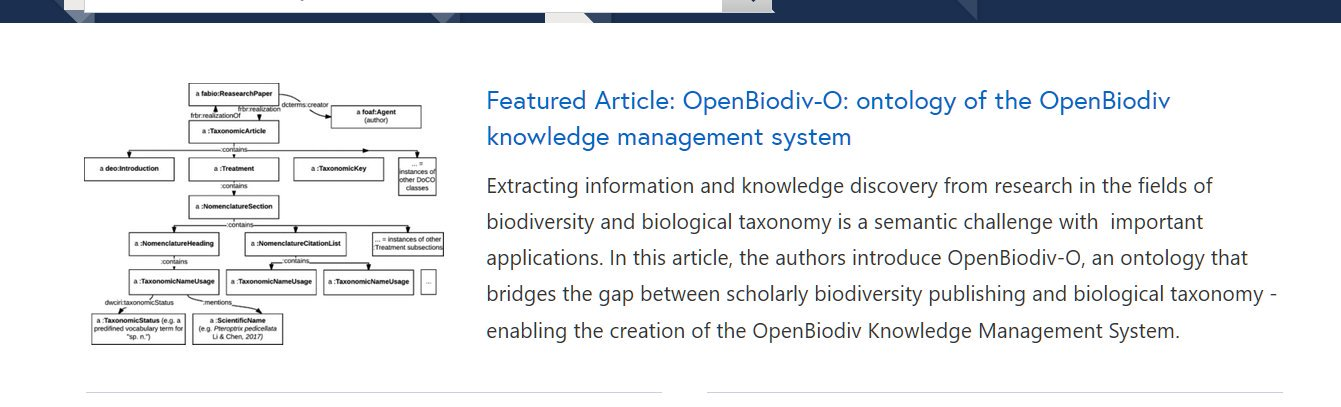
\includegraphics[width=\textwidth]{Figures/JBS-featured.jpg}
\decoRule
\caption{Статията относно OpenBiodiv-O е на началната страница на Journal of Biomedical Semantics.}
\label{fig:jbs-featured}
\end{figure}

\section*{Апробация на резултатите}
\addcontentsline{toc}{section}{Апробация на резултатите}

\subsection*{Доклади пред научен семинар на ПНЗ}
\addcontentsline{toc}{subsection}{Доклади пред научен семинар на ПНЗ}

\begin{enumerate}
    \item Доклад пред научен семинар на ИБЕИ на БАН на 26.10.2015 г. (“Публикуване, визуализация и разпространение на първични и геномни данни за биологичното разнообразие на основата на открита система за управление на информацията”).
    \item Доклад пред научен семинар в ИИКТ на БАН на 31.03.2016 г. (Open Biodiversity Knowledge Management System)
    \item Доклад пред научен семинар на ИИКТ на БАН за 23.03.2018 г. (OpenBiodiv: a knowledge-based system of biodiversity information)
\end{enumerate}

\subsection*{Доклади пред научно мероприятие в чужбина или пред международно научно мероприятие у нас}
\addcontentsline{toc}{subsection}{Доклади пред научно мероприятие в чужбина или пред международно научно мероприятие у нас}

\begin{enumerate}
    \item Доклад пред международния симпозиум EU BON в София на 23.03.2016 г. (The Data Publishing Toolkit at EU BON: Automated creation of data papers, data and text integrated publishing via the ARPHA Publishing Platform.)
    \item Доклад по време на работната среща на BIG4 в Хавраники, Чехия на 03.06.2016 г. (Project Progress Report (OBKMS))
    \item Доклад по време на работната среща на BIG4 в Хавраники, Чехия на 03.06.2016 г. (Modern Methods of Systematic Research and the BOLD Algorithm)
    \item Уеб-базиран доклад (уебинар) пред международна аудитория в рамките на семинар на iDigBio на 16.07.2016 г. (Online direct import of specimen records from iDigBio instrastructure into taxonomic manuscripts)
    \item Доклад по време на работната среща на BIG4 в Копенхаген на 14.10.2016 г. (Midterm Progress Report)
    \item Доклад на международия симпозиум TDWG 2016 в Санта Клара де Сан Карлос от 5. до 9.12.2016 г. (Streamlining the Flow of Taxon Occurrence Data Between a Manuscript and Biological Databases)
    \item Доклад на международия симпозиум TDWG 2016 в Санта Клара де Сан Карлос от 5. до 9.12.2016 г. (The Open Biodiversity Knowledge Management System: A Semantic Suite Running on top of the Biodiversity Knowledge Graph)
    \item Доклад на международия симпозиум TDWG 2016 в Санта Клара де Сан Карлос от 5. до 9.12.2016 г. (Demonstrating the Prototype of the Open Biodiversity Knowledge Management System)
    \item Доклад на международия симпозиум TDWG 2016 в Санта Клара де Сан Карлос от 5. до 9.12.2016 г. (Creation of Data Paper Manuscripts from Ecological Metadata Language (EML))
    \item Уеб-базиран доклад пред междуродния семинар на работната група по семантични технология към Университета Вандербилт (Тенеси, САЩ) на 20.02.2017 г. (Open Biodiversity Knowledge Management System)
    \item Доклад на европейската конференция на биосистематиците, BioSyst.eu 2016 на 15.08.2017 г. (The OpenBiodiv Knowledge System: The Future of Access to Biodiversity Knowledge)
    \item Доклад на международия симпозиум TDWG 2017 в Отава, Канада от 1. до 6.10.2017 г. (OpenBiodiv Computer Demo: an Implementation of a Semantic System Running on top of the Biodiversity Knowledge Graph)
    \item Доклад на международия симпозиум TDWG 2017 в Отава, Канада от 1. до 6.10.2017 г. (OpenBiodiv: an Implementaion of a Semantic System Running on top of the Biodiversity Knowledge Graph)
    \item Постер на международия симпозиум TDWG 2017 в Отава, Канада от 1. до 6.10.2017 г. (OpenBiodiv: an Implementaion of a Semantic System Running on top of the Biodiversity Knowledge Graph)
    \item Доклад по време на работната среща на BIG4 в Ла Палма, Испания от 30. окт. до 3 ноем. 2017 г. (Midterm Progress Report)
    \item Доклад пред научен семинар на групата по биоинформатика (група Ронкуист) в Кралския природо-научен музей в Стокхолм на 29.11.2017 г.
\end{enumerate}






\chapter{Резюме на глава 1: Архитектура на OpenBiodiv}
\label{chapter-openbiodiv}

В тази глава предоставяме архитектурата, т.е. спецификацията и дизайна на OpenBiodiv. Въвеждаме компонентите на OpenBiodiv, които ще бъдат разгледани подробно в следващите глави. Описваме как взаимодействат тези компоненти, за да се формира базираната на знанието система OpenBiodiv.

\section{Какво е OpenBiodiv?}

Разбирането за OpenBiodiv като система базирана на знанието може да се обобщи по следния начин: OpenBiodiv е база данни от взаимосвързана информация за биологичното разнообразие, заедно с логика и приложения, позволяващи на потребителите не само да се допитват до данните, но и да откриват допълнителни факти, свързани с данните. Основните източници на информация в OpenBiodiv са списанията на академичния издател Пенсофт, таксономичната информация от Плаци и таксономичният гръбнак на Global Information Biodiversity Facility (GBIF).

Изследователският проблем на архитектурата на OpenBiodiv може да се формулира като проектиране на семантична графична база данни на основата на RDF. Тя да е с отворен достъп и да включва информация, предоставяна от Пенсофт, Плаци и GBIF, и да позволява на потребителите на системата да задават сложни заявки.

OpenBiodiv се състои от (1) семантична графична база данни, (2) програмен код, осигуряващ функционирането на базата и (3) динамична уеб страница (front-end), улесняваща достъпа до основната база от знания (Фиг.~\ref{fig:openbiodiv-components}). OpenBiodiv позволява динамичното вмъкване на данни от хранилища за данни за биологичното разнообразие в текста на статия в Biodiversity Data Journal или друго списание, използващи фреймуорка на Пенсофт за писане на статии, ARPHA-BioDiv (\cite{penev_arpha-biodiv:_2017}). Като втора стъпка, от тези списания се извлича знание, като се възползваме от XML-схемата на тези списания (TaxPub). Списания, които са извлечени, включват ZooKeys, Biodiversity Data Journal (BDJ), PhytoKeys, MycoKeys и т.н.\footnote{Списанията могат да бъдат достъпвани под \url{https://pensoft.net/browse_journals}}. В същото време знание под формата на факти (трипъли) се извлича от Plazi TreatmentBank, архив на литература за биологичното разнообразие, съдържащ над 200 хиляди таксономични дискусии\footnote{Таксономичната дискусия е специален раздел в биологична публикация, която описва и дискутира вид или по-висок таксон. TreatmentBank е достъпен под \url{https:// //plazi.org/resources/treatmentbank/}} и актуализиран всеки ден. Не на последно място, тези факти са взаимосвързани чрез таксономичния гръбнак на GBIF (\cite{gbif_secretariat_gbif_2017}). След това извлеченото знание се съхранява в нашата семантична база данни  (Фиг.~\ref{fig:openbiodiv-sources}).

\begin{figure}
\centering
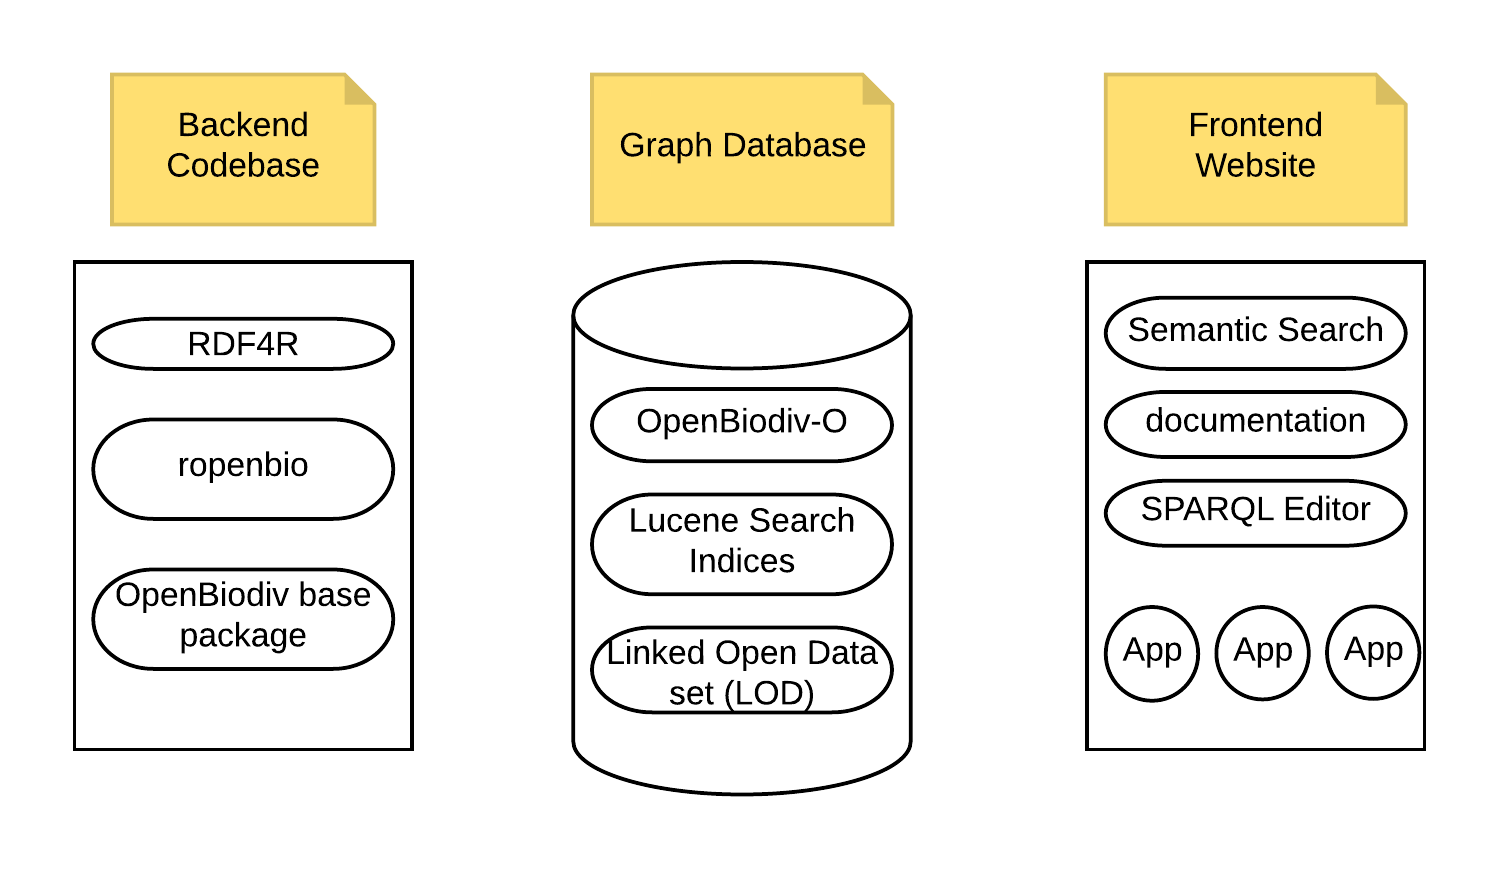
\includegraphics[width=\textwidth]{Figures/components-openbiodiv}
\decoRule
\caption[OpenBiodiv Components]{Компоненти на OpenBiodiv.}
\label{fig:openbiodiv-components}
\end{figure}

\begin{figure}
\centering
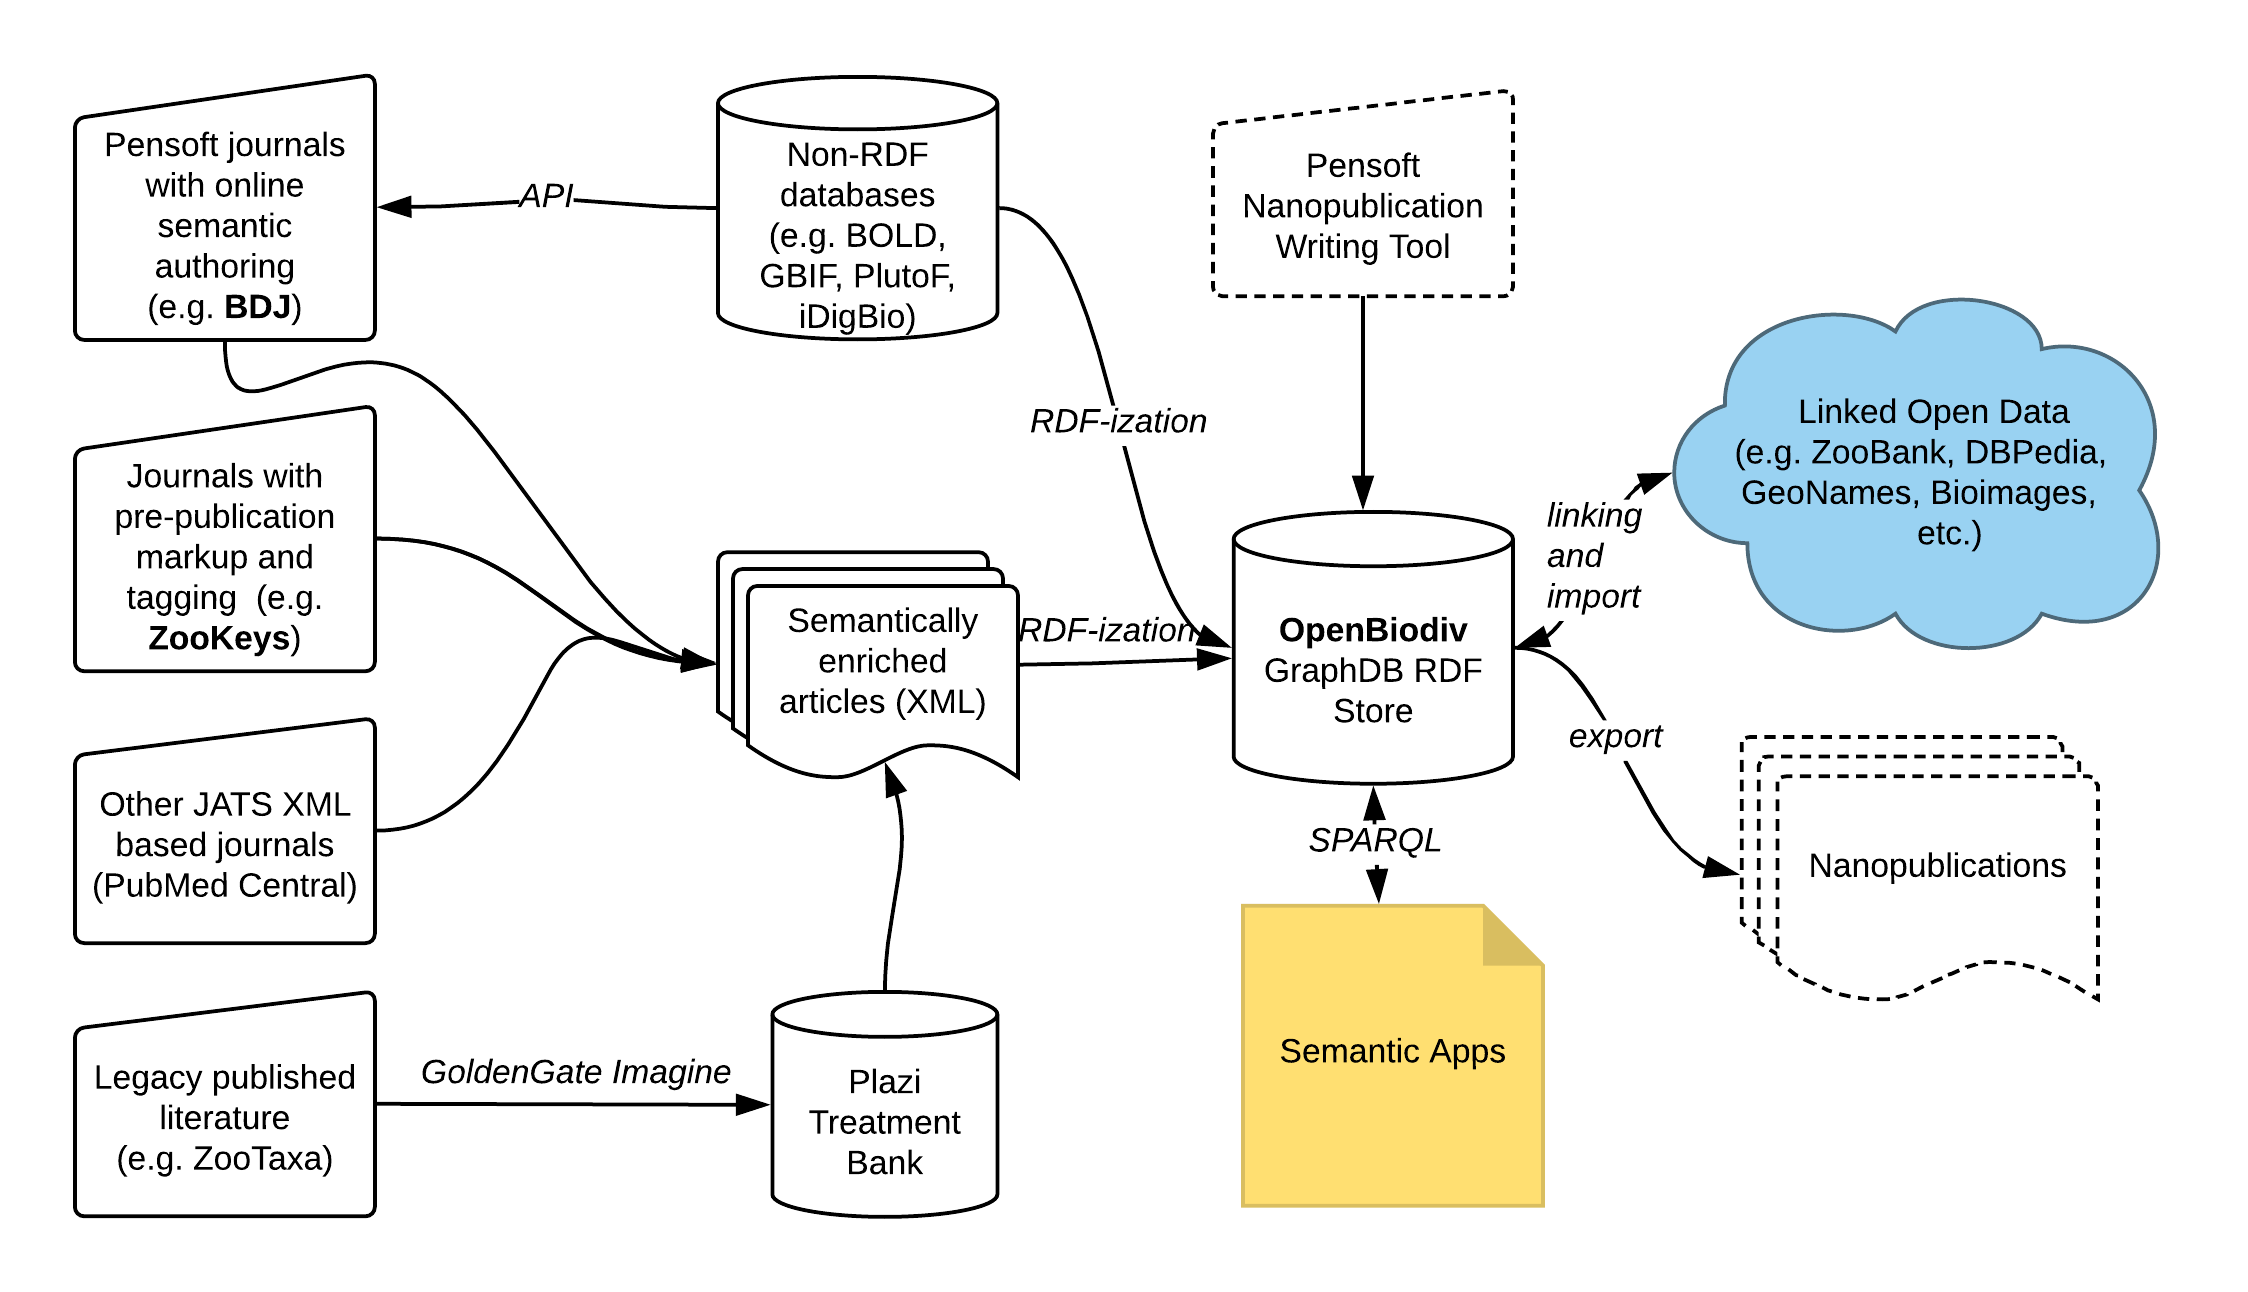
\includegraphics[width=\textwidth]{Figures/openbiodiv-sources}
\decoRule
\caption[OpenBiodiv Components]{Поток на информация в пространството за данни за биологичното разнообразие. Пунктираните линии са компоненти, които все още не са създадени.}
\label{fig:openbiodiv-sources}
\end{figure}

\section{Семантична база данни}

Основен резултат от усилията на OpenBiodiv е създаването на семантична база данни, базирана на знания, извлечени от архивите на Пенсофт и Плаци и таксономичния гръбнак на GBIF и достъпни под \url{http://graph.openbiodiv.net/}. Следва обсъждане на компонентите на базата данни.

\subsection{Онтология OpenBiodiv-O}

Централният резултат от усилията по OpenBiodiv е създаването на формален модел на областта за публикуването на знание за биоразнообразието. Този формален модел е онтологията OpenBiodiv-O (\cite{senderov_openbiodiv_2017}). Изходният код на онтологията и придружаващата документация могат да бъдат достъпвани под \url{https://github.com/pensoft/openbiodiv-o}. Детайлна дискусия е представена в глава~\ref{chapter-ontology}.

\subsection{Свързани отворени данни OpenBiodiv-LOD }

Използвайки OpenBiodiv-O и инфраструктурата, описана по-нататък в тази глава, са създадени свързани отворени данни, включващи приблизително 200 хиляди записа от Плаци, пет хиляди статии от Пенсофт, както и таксономичия гръбнак на GBIF (над милион биологични имена). Данните са достъпни онлайн чрез работния инструмент на семантичната база данни \url{http://graph.openbiodiv.net}. Разясняват се подробно в глава~\ref {chapter-lod}.

\section{Backend}

За да се попълва семантичната база данни, е необходимо да се създаде инфраструктура, която преобразува необработени данни (текст, изображения, таблици с данни и т.н.) в структуриран семантичен формат. OpenBiodiv предоставя инфраструктура за трансформиране на научни публикации за биоразнообразието в твърдения под формата на RDF с помощта на инструментите, описани в този раздел.

\subsection{RDF4R: R пакет за работа с RDF}

Едно от по-големите технически предизвикателства за OpenBiodiv е трансформирането на информация за биологичното разнообразие (напр. таксономични имена, метаданни, фигури и т.н.), съхранявани като полу-структуриран XML в напълно структурирани семантични знания под формата на RDF. За да се реши това предизвикателство, е разработен R пакет, който позволява създаването, манипулирането и записа в семантична база данни на създадения RDF. Този пакет е достъпен под лиценз с отворен код на GitHub под \url{https://github.com/vsenderov/rdf4r}. Описваме пакета в глава~\ref{chapter-rdf4r}.

\subsection{Базисен програмен код и ROpenBio}

В комбинация с пакета RDF4R, програмният код съдържа още един R пакет, \cl{ropenbio} и базисен програмен код от скриптове и документация, необходими за стартиране на базата данни. \cl{ropenbio} използва пакета RDF4R за преобразуване на полу-структуриран XML в RDF. Той съдържа преобразуванията, необходими за тази реализация. Той е достъпен под \url{https://github.com/pensoft/ropenbio}. Базисният софтуерен код координира извикването на \cl{ropenbio}, съдържа скриптове за автоматично импортиране на нови ресурси и други подробности. Той е достъпен под \url{https://github.com/pensoft/openbiodiv}. Генерирането на OpenBiodiv-LOD с помощта на тези пакети е обсъдено в глава~\ref{chapter-lod}.

\subsection{Работен процес за преобразуване на екологични метаданни в ръкопис}

Език за екологични метаданни (EML) е популярен формат за описване на екологични данни (\cite{michener_nongeospatial_1997}). Хранилища на данни за биоразнообразието, като GBIF и DataOne, използват този формат за метаданните, които съхраняват. Автоматичното преобразуване на EML файл в data paper ръкопис от Biodiversity Data Journal\footnote {Data paper (\cite{chavan_data_2011}) е научна статия, обсъждаща научни данни.} е възможно с помощта на системата OpenBiodiv (\cite{senderov_online_2016}). Този работен процес е описан подробно в глава~\ref{chapter-case-study}\footnote{За работа в интерактивен режим, отидете на \url{https://arpha.pensoft.net}, влезте в системата (регистрацията е безплатна), изберете ``Start a new manuscript'', превъртете до ``Import manuscript'' и следвайте необходимите стъпки, за да качите EML файл и да го използвате като шаблон за вашия нов ръкопис.}.

\subsection{Работен процес за импортиране на данни за наблюдения на видове в ръкопис}

Един от важните видове данни за биологичното разнообразие са данни за наблюдения на организми, occurrence data. Това са данни, които документират наличието на правилно таксономично идентифициран организъм на дадено място и време. Такива данни се съхраняват в международни хранилища като BOLD, GBIF, PlutoF и iDigBio. За да се улесни публикуването на такъв тип данни е разработен работен процес за импортиране на такива записи от тези бази данни в таксономична статия (taxonomic paper) в списанието Biodiversity Data Journal (\cite{senderov_online_2016}). Този работен процес е описан подробно в глава~\ref{chapter-case-study}\footnote{За да отворите интерактивно работния процес, отидете на \url{https://arpha.pensoft.net}, влезте в системата (регистрацията е безплатна), изберете ``Start a new manuscript'', изберете ``Biodiveristy Data Journal'', ``Taxonomic paper''  и ``Create a new manuscript''. След това в новия ръкопис щракнете с мишката върху раздела ``Taxon treatments'', като кликнете върху знака $+$ до него, и укажете биологичната класификация на новия запис (напр. Animalia), и най-накрая щракнете върху ``Save'' и ще ви бъде представен избор на подраздели. Кликнете върху секцията ``Materials'' от-вляво, за да видите инструмента на работния процес за вмъкване на материли. Погледнете в долната част на диалоговия прозорец, където можете да поставите множество идентификационни номера. Това е частта, в която избирате външни идентификатори на ресурси, които да бъдат импортирани във вашата статия.}.

\section{Интерфейс}

В допълнение към предоставения endpoint за база данни с възможност за търсене, се разработва уебсайт, позволяващ семантично търсене и капсулиращ специфични задачи, пакетирани като приложения (\url{http://openbiodiv.net}). Бета версията вече е в действие. Фиг.~\ref{fig:website}. Ограничена дискусия е представена в глава~\ref{chapter-webportal}.

\section{Системна администрация}

Системата е разположена на виртуална машина на Debian GNU+Linux. GraphDB работи с heap файл от 20 GB и с набор от правила RDFS-Plus Optimized. Това се налага поради факта, че достигнахме препятствия, когато използвахме OWL извод. Обсъдени в глава~\ref {chapter-lod}. Непрекъснатата работа се осигурява от автоматичното изпълнение на скриптове от директорията \cl{run} на базисния код на OpenBiodiv.

\begin{figure}
\centering
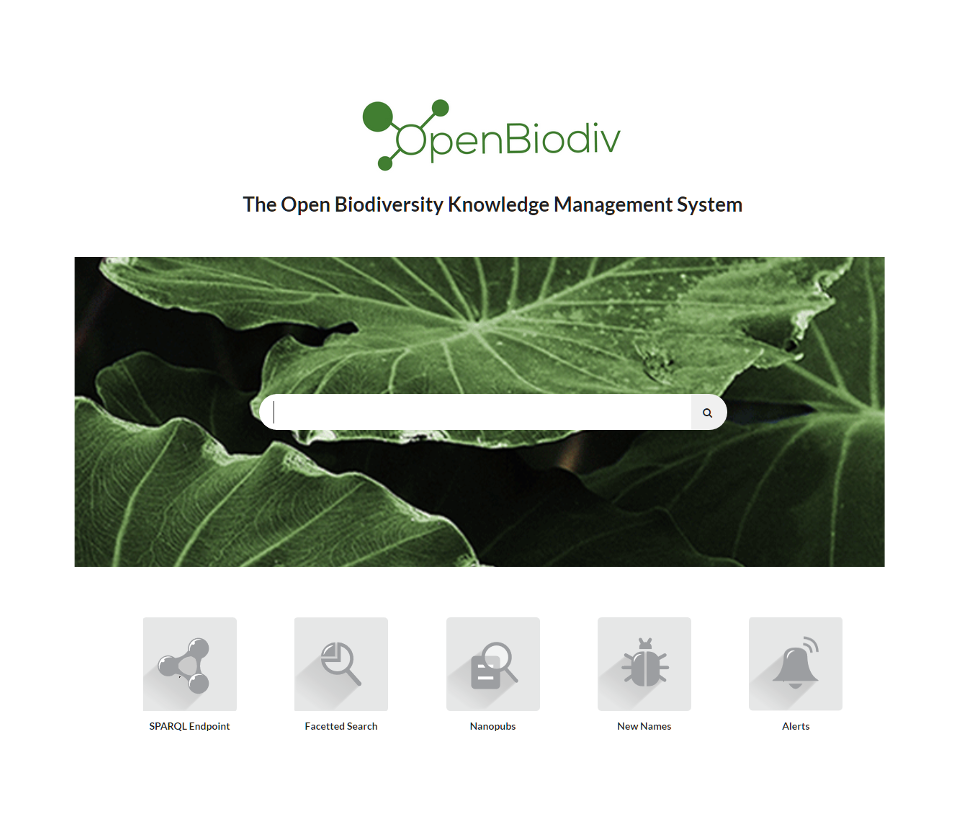
\includegraphics[width=\textwidth]{Figures/openbiodiv-webpage}
\decoRule
\caption[OpenBiodiv Website]{Бета версия на потребителския интерфейс.}
\label{fig:website}
\end{figure}

\section{Дискусия}

Проектирането на системата започна във втората половина на 2015 г., когато бяха разгледани различни алтернативи за база данни (Neo4J, GraphDB, WikiBase) и различни технологии за RDF-изация на знание. Освен това беше направен избор на източници за информация и типове данни, които са интересни. Бяха разгледани основните модели данни и онтологии. След този анализ, публикувахме спецификацията на системата в \cite{senderov_open_2016} като отворен проект за дисертация (PhD project plan). По време на имплементацията обаче се оказа, че първоначалният план не отговаря на изменящите се изисквания на системата и на новите предизвикателства, които възникваха по време на имплементацията. По тази причина през втората и третата година на усилията за създаване на OpenBiodiv преминахме от модела на разработка waterfall, където след първоначален етап на изготвяне на софтуерната архитектура се преминава към продължителен етап на имплементация и тестване към модела agile, където спецификацията е разбита на по-малки user-stories, които биват реализирани ad-hoc в рамките на едно- или двумесечни спринтове. Например, за разработването на софтуерната библиотека за RDF-изация RDF4R, user-stories са ``възможност за работа с литерали'', ``възможност за импортиране през API endpoint'' и т.н. Първоначалният страх, че това ще доведе до ``хакерски код'' и недобре организирана софтуерна архитектура се оказа неоправдан, защото при изолирането на проблемите един от друг, успявахме да се концентираме върху проблемите последователно и да ги решаваме по елегантен начин. Аспекти на методологията agile, от които не успяхме да се възползваме напълно бяха колаборативните аспекти, може би поради факта, че системата беше разработена основно от кандидата със съдействието на един от програмистите на Пенсофт; в класическия смисъл на понятието agile team не съществуваше. По тази причина не практикувахме повечето ритуали като stand-ups и retrospection, а основно се концентирахме върху интеративния характер на разработката на софтуер.

Нашата визия за бъдещето на системата е работата по нея да се поеме от agile team, който да се възползва от пълния арсенал на методологията.
\chapter{Резюме на глава 2: Онтологията на OpenBiodiv}
\label{chapter-ontology}

OpenBiodiv трансформира информация за биоразнообразието от научни публикации и академични бази данни в семантичен вид. В тази глава представям OpenBiodiv-O (\cite{senderov_openbiodiv-o:_2018}) - онтологията, формираща модела на OpenBiodiv за знания и извод. OpenBiodiv-O предоставя концептуален модел на структурата на академична публикация в сферата на биоразнообразието и на съдържаните в нея таксономични концепции. За първи път формално е концептуализирана областта на публикуването на данни за биоразнообразието.

Чрез разработването на онтология, насочена към биологичната таксономия са запълнени празнините между онтологии като Darwin-SW и онтологиите за семантично публикуване като онтологиите SPAR. Считам, че е предимство да се моделира самият таксономичен процес, а не някакво конкретно състояние на знанието.

Изходният код и документацията са достъпни под лиценза CC BY \footnote {Creative Commons Attribution 4.0 International Public License} от GitHub \footnote {\url{https://github.com/vsenderov/openbiodiv-o/blob/master/LICENSE.md}}. Започваме с увод в областта на биологичната таксономия и свързаните с нея биоразнообразие.

\section{Концептуализация на областта}

Представям историята на модерната биологична таксономия, като се започне с Карл Линней (1707-1778), който предложи модерното групиране на организма на \emph{царства, класове, разреди, родове} и използването на латинските биномични имена в \emph{Systema Naturae} (\cite {linnaeus_systema_1758}). Подчертавам, че работата на таксономите за описване и организиране на биоразнообразието далеч не е пълна. Това информира създаването на новата онтология не като статично формализиране на съществуващата биологична таксономия в компютърно четима форма, а като формализиране на \emph{научния процес на биологичната таксономия}.

След това описвам подробно, как протича научният процес в биологичната таксономия. Започвам с въвеждането на таксономични концепции и начина, по който се формират. Таксономичната концепция е научна хипотеза (\cite{deans_time_2012}), че определена група от организми съществува в природата. Тя се формира чрез изследване на екземпляри и задължително включва научен критерий по който те да се групират, често наричан видова концепция (\cite {mallet_species_2001}) Исторически погледнато, организмите могат да бъдат групирани по външен вид и вътрешно устройство (концепция за морфологични видове) или репродуктивно поведение (биологична видова концепция), но напоследък фокусът се е насочил към групиране въз основа на генетична свързаност (филогенетични и геномни видови концепции).

След това описвам единците на биологичната таксономия и начина, по който те са регламентирани от международните кодекси \cite{international_commission_on_zoological_nomenclature_international_1999, noauthor_international_2012}). Кодексите уреждат по-ниските рангове: видове, род, семейство, разред; по-високите рангове (напр. отдел, царство, домейн и т.н.) могат да бъдат използвани от изследователите, както сметнат за подходящо. Това води до множество конкуриращи се гледни точки.

Публикуването таксономични концепции е неразделна стъпка в научния работен поток на всеки таксоном. Описваме структурата и типовете таксономични публикации, като се акцентираме специално върху секцията ``Таксономична дискусия'', раздела в таксономичната публикация, където таксономичната концепция е дефинирана.

\subsection*{Преглед на литературата}

В тази секция се разглеждат опитите областта на биологичната таксономия да бъде формално концептуализрана.  Интересни са SPAR Ontologies, \cite{peroni_semantic_2014}) и TaxPub XML Document Type Definition (\cite{catapano_taxpub:_2010}).

Концептуализацията основно е повлияна освен от практиката и от кодексите (\cite{international_commission_on_zoological_nomenclature_international_1999,noauthor_international_2012}), а така и от стандартите, създадени от TDWG (напр. Darwin Core, DwC, \cite{wieczorek_darwin_2012}).

Накрая правим обзор на областта на концептуалната таксономия (\cite{berendsohn_concept_1995, franz_perspectives:_2009,sterner_taxonomy_2017}), която представлява нова гледна точка за това, как трябва да протича процесът на опсване на видове в биологичната таксономия, с оглед на напредъка на информационните технологии.

\section{Методи}

OpenBiodiv-O се изразена посредством RDF чрез използване на RDF Schema (RDFS) и Web Ontology Language (OWL).

За да разработим онтологията ние използвахме следния процес: (1) анализ на областта и идентифициране на важните класове обекти и техните взаимоотношения (наричани свойства); (2) анализ на съществуващите информационни модели и онтологии и идентифициране на липсващите класове и свойства за успешно формализиране на областта.

\section{Резултати}

OpenBiodiv-O е \emph{споделена формална спецификация на концептуализация} на областта на биоразнообразието по смисъла на \cite{gruber_translation_1993, obitko_translations_2007, staab_handbook_2009}. Тяхното разбиране за онтология сме въвели в Background. 

Има няколко домейна, в които моделираните ресурси падат. Първият е научната област за публикуване на данни за биоразнообразието. Втората област е тази на таксономичната номенклатура. Третата област е на по-широката таксономия (например таксономични понятия и техните взаимоотношения, видови събития, черти).

\subsection{Семантично моделиране на домейна за публикуване на данни биоразнообразието}

Разширяваме рамката на онтологиите на SPAR, като въвеждаме нова категория за таксономичните статии, нейните подраздели, както и нов клас за споменаване на таксономично име (вж. следващ подраздел). Тези нови класове са обобщени в Таблица~\ref{bibliographic_classes}.

\begin{table}[h!]
\caption{Нови класове в областта на публикуването на данни за биоразнообразието.}
      \begin{tabular}{cc}
        \hline
          Class QName             & Comment\\  \hline
  {\tt :Treatment}                & section of a taxonomic article\\
  {\tt :NomenclatureSection}      & subsection of Treatment\\
  {\tt :NomenclatureHeading}      & contains a nomenclatural act \\
  {\tt :NomenclatureCitationList} & list of citations of related concepts\\
  {\tt :MaterialsExamined}        & list of examined specimens\\
  {\tt :BiologySection}           & subsection of Treatment\\
  {\tt :DescriptionSection}       & subsection of Treatment\\
  {\tt :TaxonomicKey}             & section with an identification key\\
  {\tt :TaxonomicChecklist}       & section with a list of taxa for a region\\ 
  {\tt :TaxonomicNameUsage}       & mention of a taxonomic name\\ \hline

      \end{tabular}
      \label{bibliographic_classes}
\end{table}

Графичното представяне на взаимоотношенията между ресурси на класовете, свързани с публикуването, които OpenBiodiv въвежда, може да се намери в диаграмата на фиг.~\ref{taxonomic-article-diagram}.

\begin{figure}[h!]
	\centering
	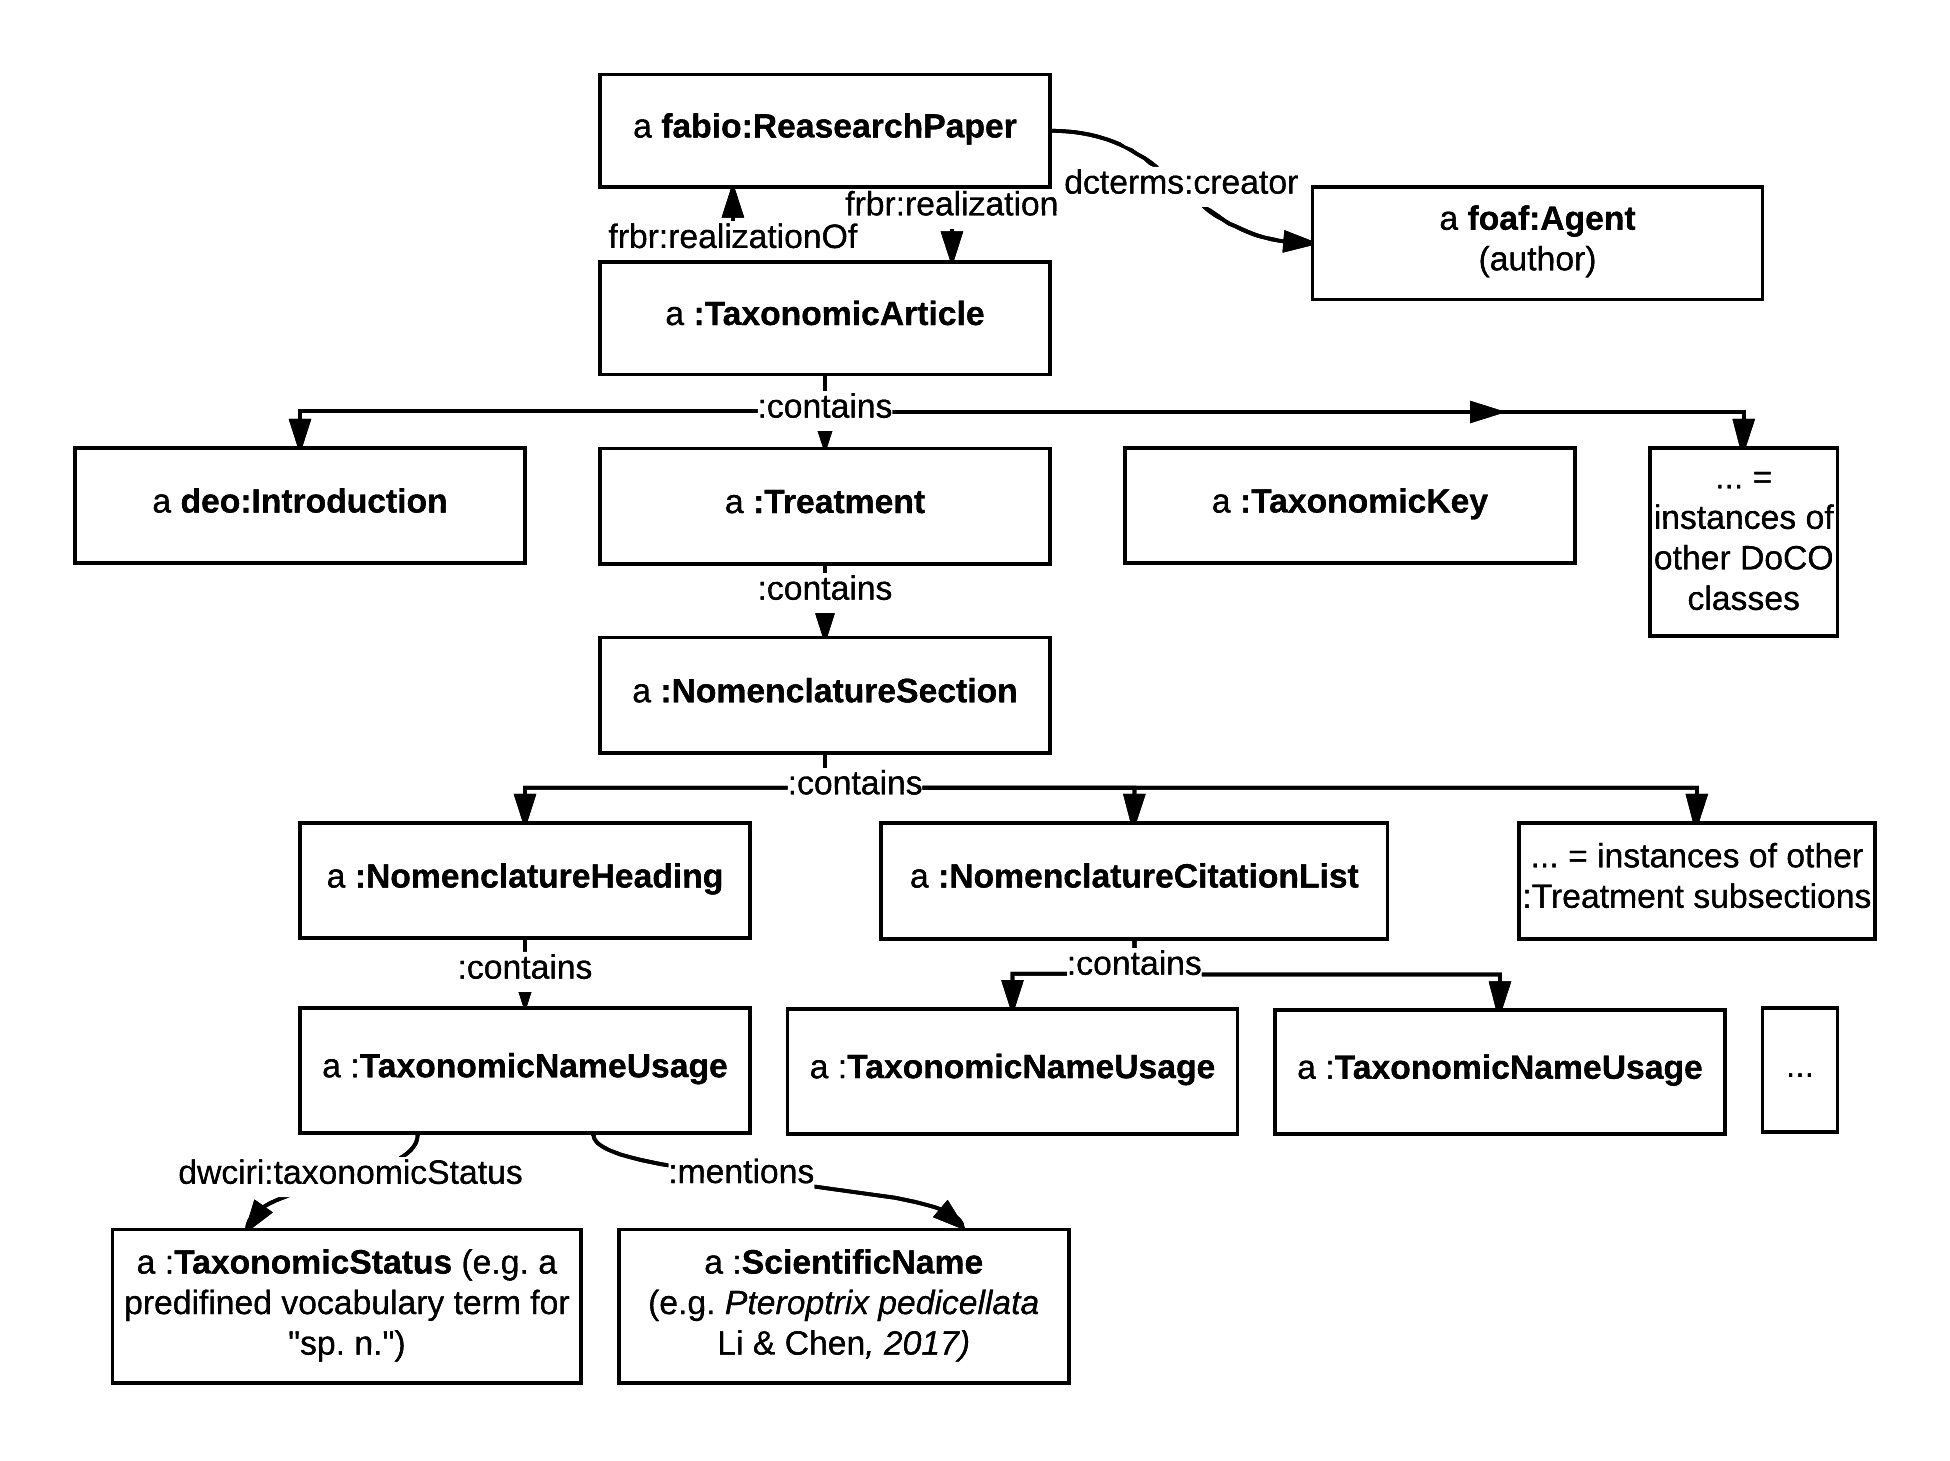
\includegraphics[width=\textwidth]{Figures/taxonomic-article-diagram}
	\decoRule
  \caption[Taxonomic article diagram.]{Графична репрезентация на взаимоотношенията между ресурсите, които OpenBiodiv въвежда за публикуване на данни за биоразнообразието.}
  \label{taxonomic-article-diagram}
\end{figure}

\subsubsection{Семантика и употреба}

В тази секция ние обсъждаме как класовете и свойствата, които въведохме, са в съответствие с модела на функционалните изисквания за библиографски записи (FRBR), използван от SPAR. Считаме дадена таксономична статия за конкретен израз/запис, FRBR Expression, на абстрактното понятие работа, FRBR Work, представляващо интелектуалното съдържание на статията. Таксономичната дискусия се третира подобно на Въведение, Методи, Резултати и т.н., т.е. също e FRBR Expression и DEO discourse element. Таксономична концепция е съответният абстрактен ресурс от клас FRBR Work на дадена таксономична дискусия. Фигурите~\ref{example-article-metadata} и \ref{example-article-structure} дават примерен сорс-код, илюстриращ тези идеи.

\begin{figure}[h!]
	\centering
	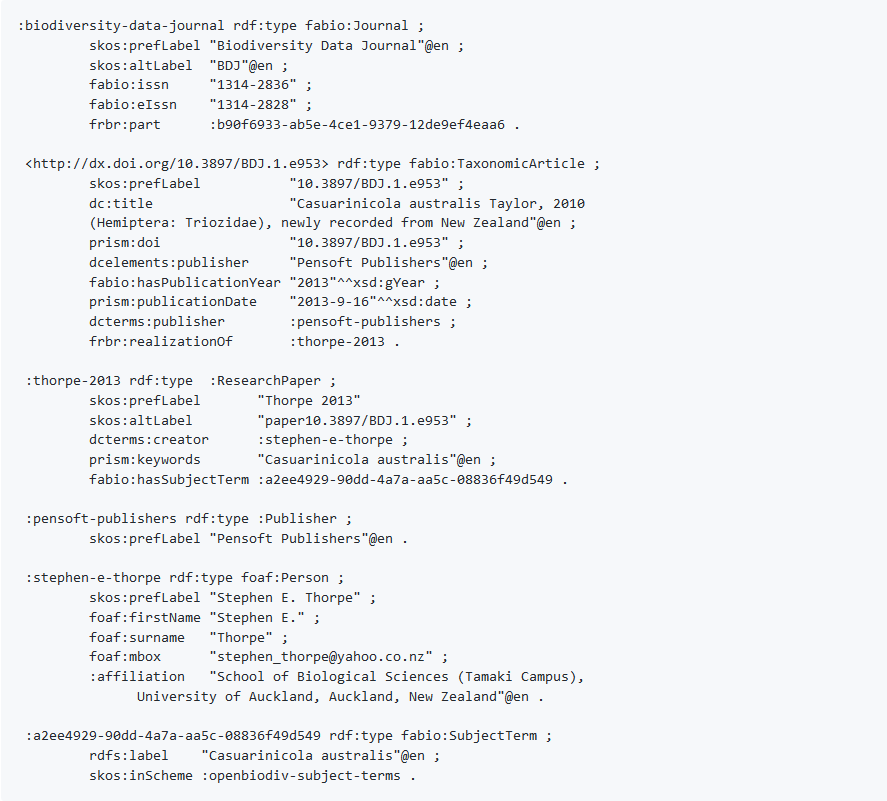
\includegraphics[width=\textwidth]{Figures/example-article-metadata}
	\decoRule
  \caption[Example article metadata.]{Този пример показва как да се изразят метаданните на таксономичната статия с модела на SPAR Ontologies и класовете, които OpenBiodiv определя. Кодът е на Turtle.}
  \label{example-article-metadata}
\end{figure}

\begin{figure}[h!]
  \centering
  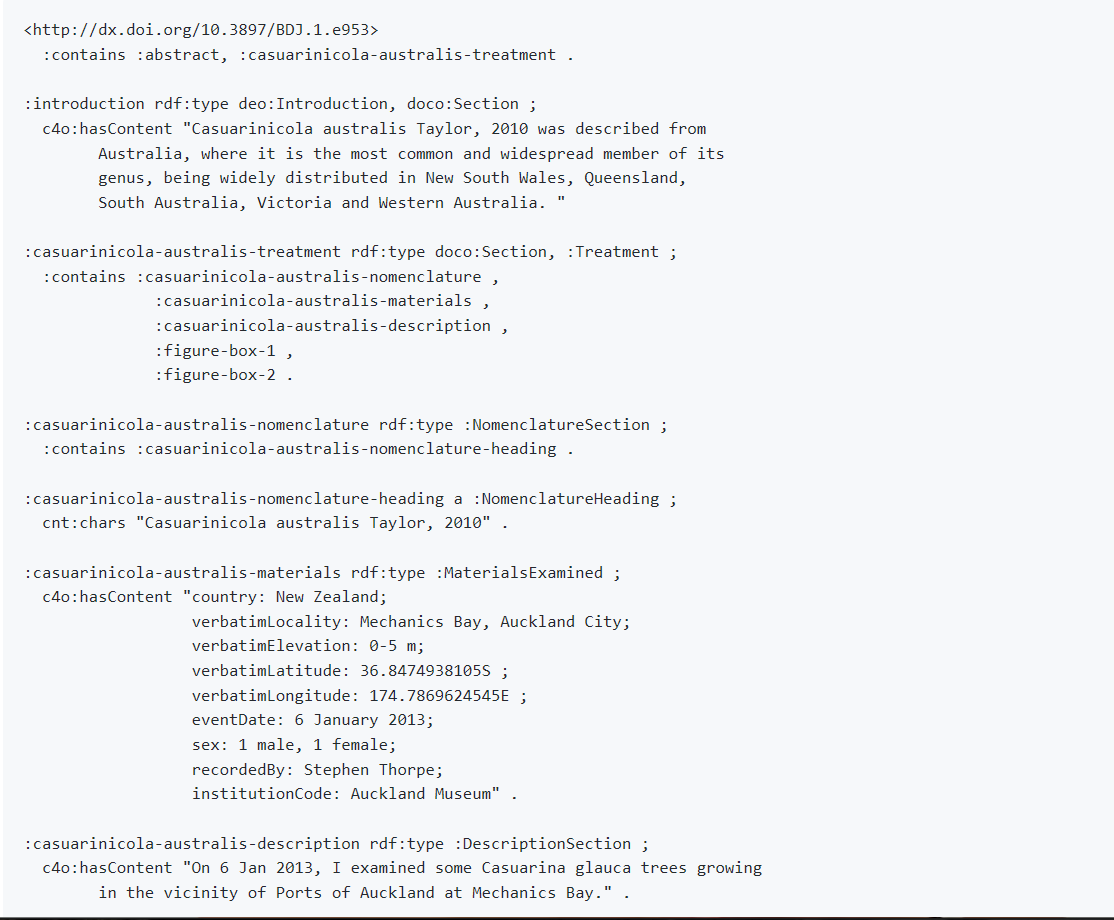
\includegraphics[width=\textwidth]{Figures/example-article-structure}
  \decoRule
  \caption[Example article structure.]{Този пример показва как да изразява структурата на статията с помощта на \cl{contains}. Кодът е на Turtle.}
  \label{example-article-structure}
\end{figure}


\subsection{Семантично моделиране на биологичната номенклатура}

Биологичната номенклатура е система с над 200 годишна традиция датираща до преди времето на информатиката и дори до преди времето на Теорията за еволюцията на Дарвин. Много е трудно да се моделира поради сложността си и само частично е обхваната от онтологиите NOMEN и TNSS (въведени в подраздел ``Previous Work''). С OpenBiodiv-O използвам подход "отдолу-нагоре" за моделиране на използването на таксономични имена в статиите. Където е възможно, ние подравняваме класовете OpenBiodiv-O на NOMEN.

Дефинирахме йерархията на класовете на таксономичните имена, намиращи се на фиг.~\ref{taxonomic-name-class-hierarchy-diagram}. Освен това въведехме taxonomic name usage (\cl{TaxonomicNameUsage}).

\begin{figure}[h!]
  \centering
  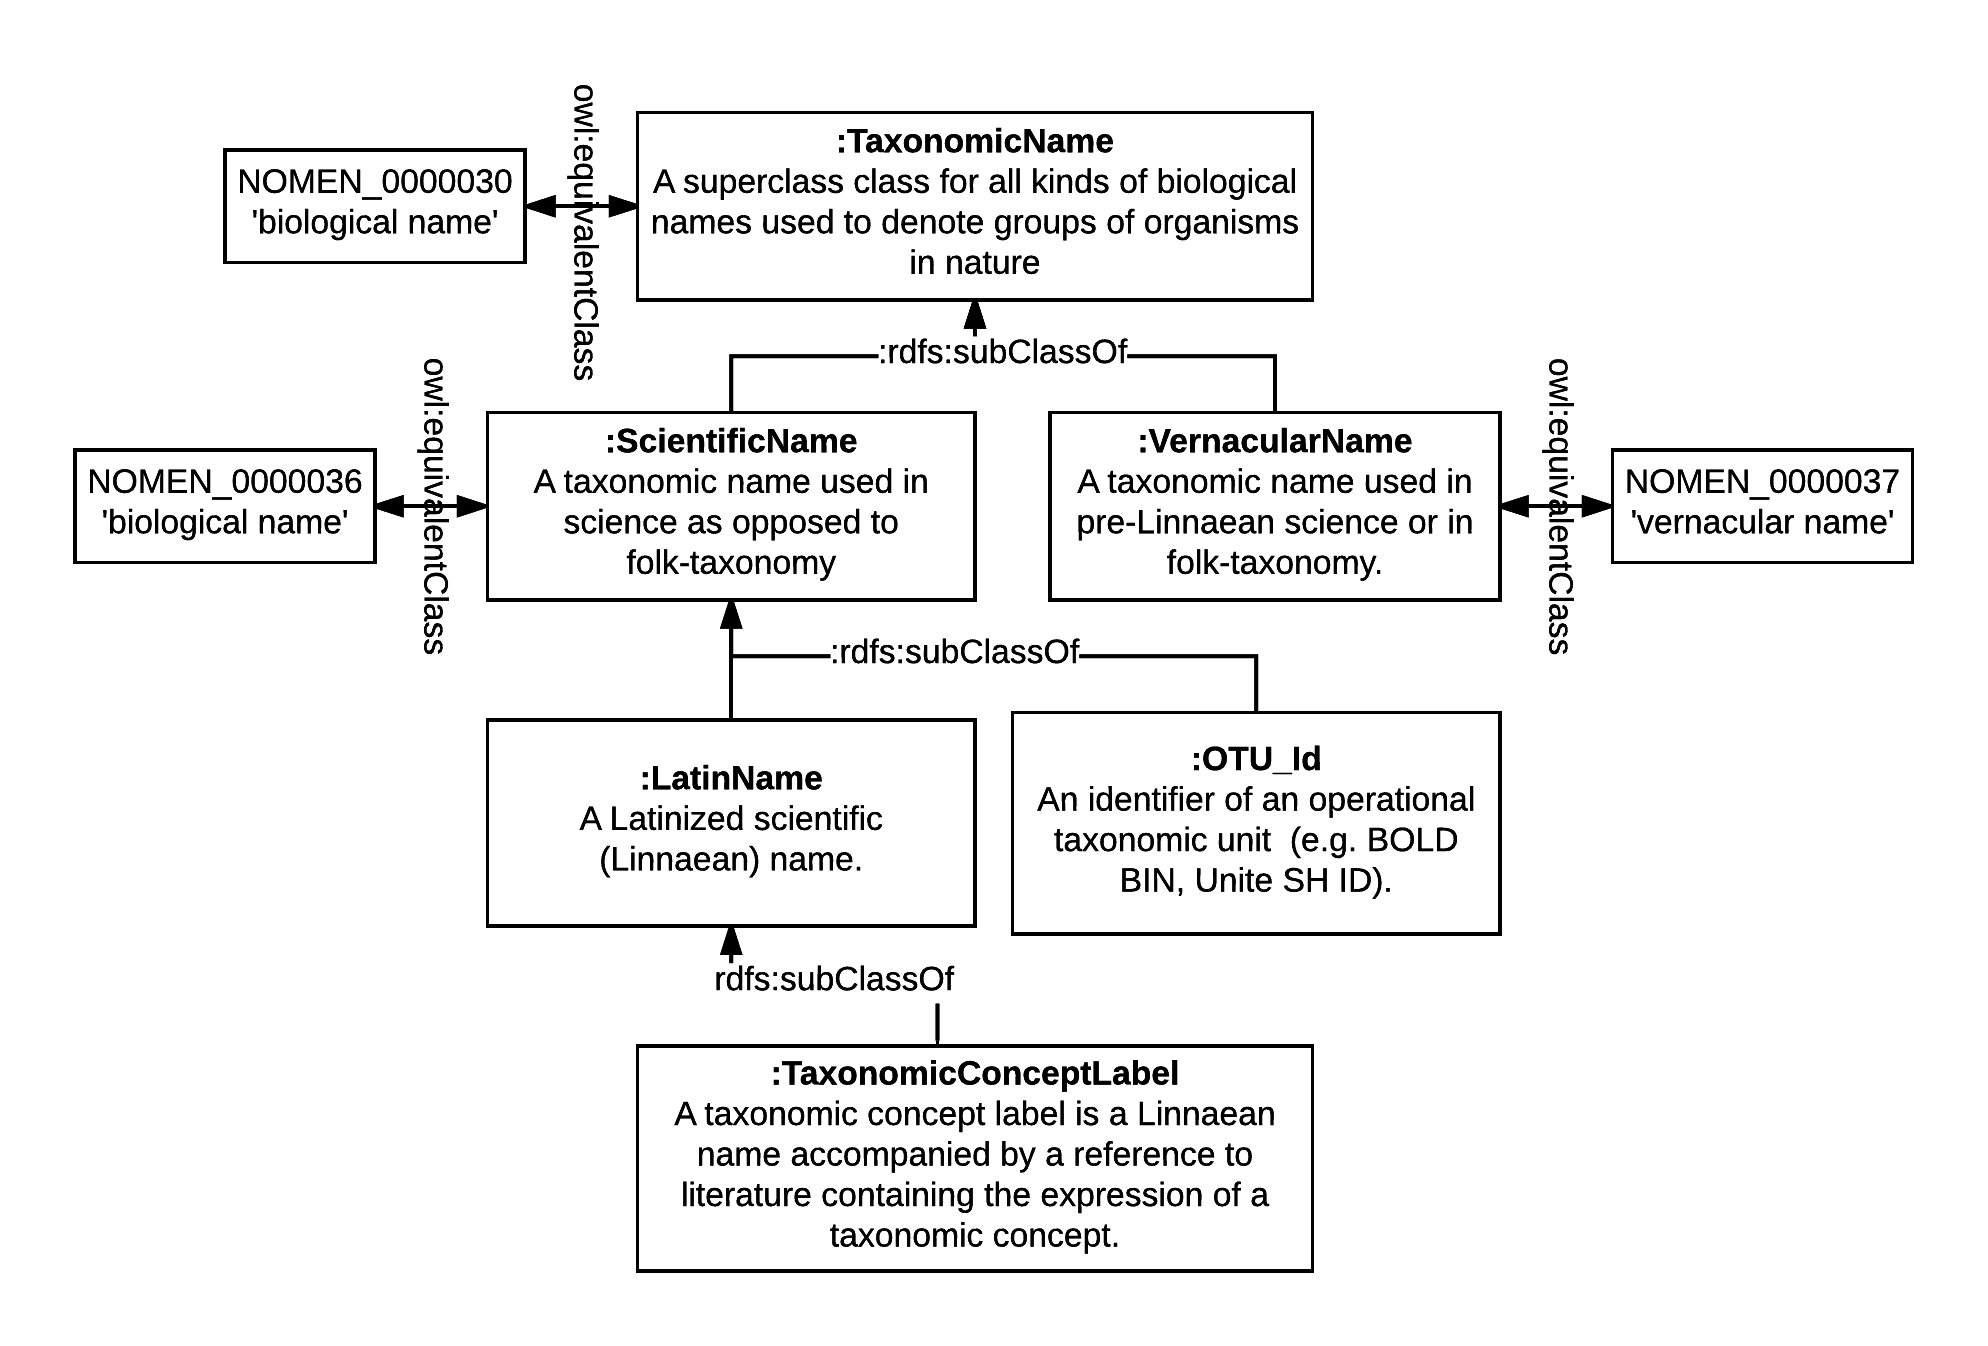
\includegraphics[width=\textwidth]{Figures/taxonomic-name-class-hierarchy-diagram}
  \decoRule
  \caption[Taxonomic name class hierarchy diagram.]{Създадохме тази йерархия, за да приспособим както традиционните таксономични наименования, така и използването на таксономични концептуални етикети и оперативни таксономични единици.}
  \label{taxonomic-name-class-hierarchy-diagram}
\end{figure}

Въвеждаме Taxonomic Concept Label (\cl{TaxonomicConceptLabel}). Етикетът на таксономична концепция (TCL) е линеево име плюс позоваване на публикация, където дискутираният таксон е дефиниран. Връзката се осъществява чрез ключовата дума ``sec.'' (Латинки за (\emph{secundum} \cite{berendsohn_concept_1995}). Напр. \emph{Andropogon virginicus} var. \emph{tenuispatheus} \cite{blomquist_grasses_1948}. Тук \cite{blomquist_grasses_1948} е валидна библиографска справка за публикацията, в която концепцията е дефинирана.

Извадихме съкращения от таксономични термини от около 4000 статии в четири таксономични списания (ZooKeys, Biodiversity Data Journal, PhytoKeys и MycoKeys), за да създадем таксономичен речник на термините, който обхваща осемте най-често срещани случая Таблица~\ref{taxonomic-status-vocabulary}). Латинските съкращения, които са класифицирани в тези класове, могат да бъдат намерени на страницата на OpenBiodiv-O GitHub. (Вижте Методи за повече подробности).

\begin{table}[h!]
\caption{Речник с таксономични термини.}
\begin{tabular}{ccc}
\hline
Vocabulary Instance QName & Example Abbrev & Comment\\ \hline
{\tt :TaxonomicUncertainty} & \emph{incertae sedis} & Taxonomic Uncertainty\\
{\tt :TaxonDiscovery} & \emph{sp. n.} & Taxonomic Discovery \\
{\tt :ReplacementName} & \emph{comb. n.} & Replacement Name \\
{\tt :UnavailableName} & \emph{nomen dubium} &  Unavailable Name \\
{\tt :AvailableName} & \emph{stat. rev.} & Available Name \\
{\tt :TypeSpecimenDesignation} & \emph{lectotype designation} & Type Specimen Designation \\
{\tt :TypeSpeciesDesignation} & \emph{type species} & Type Species Designation\\
{\tt :NewOccurrenceRecord} & \emph{new country record} & New Occurrence Record (for region)\\
\hline
\end{tabular}
\label{taxonomic-status-vocabulary}
\end{table}

Въз основа на нашия анализ на термините за таксономични статуси, идентифицирахме два модела за съответствие между кодирането на латинизираните научни имена (Фиг.~\ref{scientific-name-patterns}). Моделът \emph{заместващо име}, изпълняван чрез свойството \cl{replacementName}, показва, че вместо едно латинизирано име,  трябва да се използва друго. Тя обхваща голямо разнообразие от случаи в кодексите, като например поставянето на един вид таксон в нов род (нова комбинация), поправката на наименование поради номенклатурни причини (ново име), или прилагането на Принципа на приоритет за откриването на синоними ("syn nov.", \cite{international_commission_on_zoological_nomenclature_official_2017}).

\begin{figure}[h!]
 \centering
  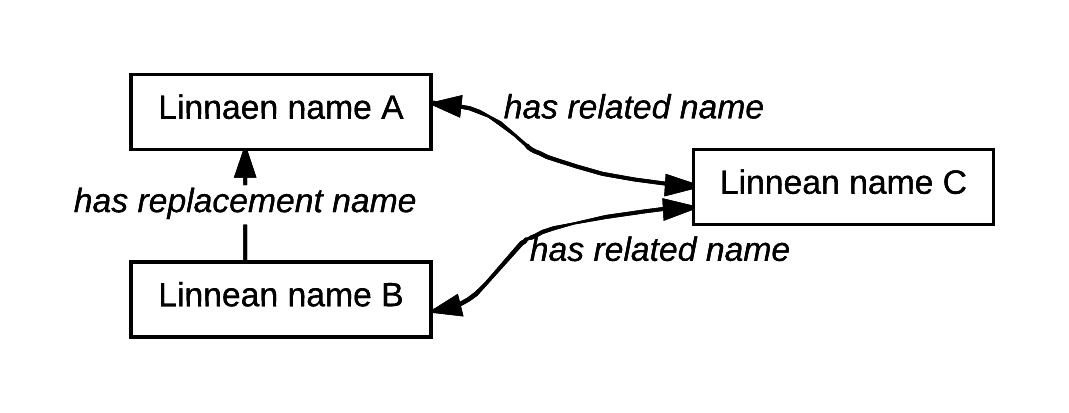
\includegraphics[width=\textwidth]{Figures/scientific-name-patterns}
  \decoRule
  \caption[Scientific name patterns diagram.]{
  Веригите на \emph {заместващи имена} могат да бъдат проследени, за да се намери използваното понастоящем име. \emph{Свързано име} показва, че две имена са свързани по някакъв начин, но не кой е предпочитан.}
  \label{scientific-name-patterns}
\end{figure}

Другият модел е този на \emph{свързани имена} (\cl{relatedName}). Това е по-широк модел, който показва, че две имена са някак си свързани. Например, те могат да бъдат синоними, едното да замества другото, или да сочат към таксономично свързани таксономични понятия. Например, \emph{Harmonia manillana} (\cite{mulsant_monographie_1866}) е свързано с \emph{Caria manillana} \cite {mulsant_monographie_1866} \emph{Harmonia manillana} (според \cite{poorani_harmonia_2016} лектотипус на \emph{Harmonia manillana} (\cite{mulsant_monographie_1866}) sec. \cite{poorani_harmonia_2016} носи името \emph{Caria manillana} \cite{mulsant_monographie_1866}).

\subsubsection{Семантика и употреба}

Както се вижда от фиг.~\ref{taxonomic-name-class-hierarchy-diagram}, таксономичните имена на OpenBiodiv-O са приравнени към NOMEN имена. Илюстрации в примера на Фиг.~\ref{example-taxonomic-name-usage}.

\begin{figure}[h!]
\centering
  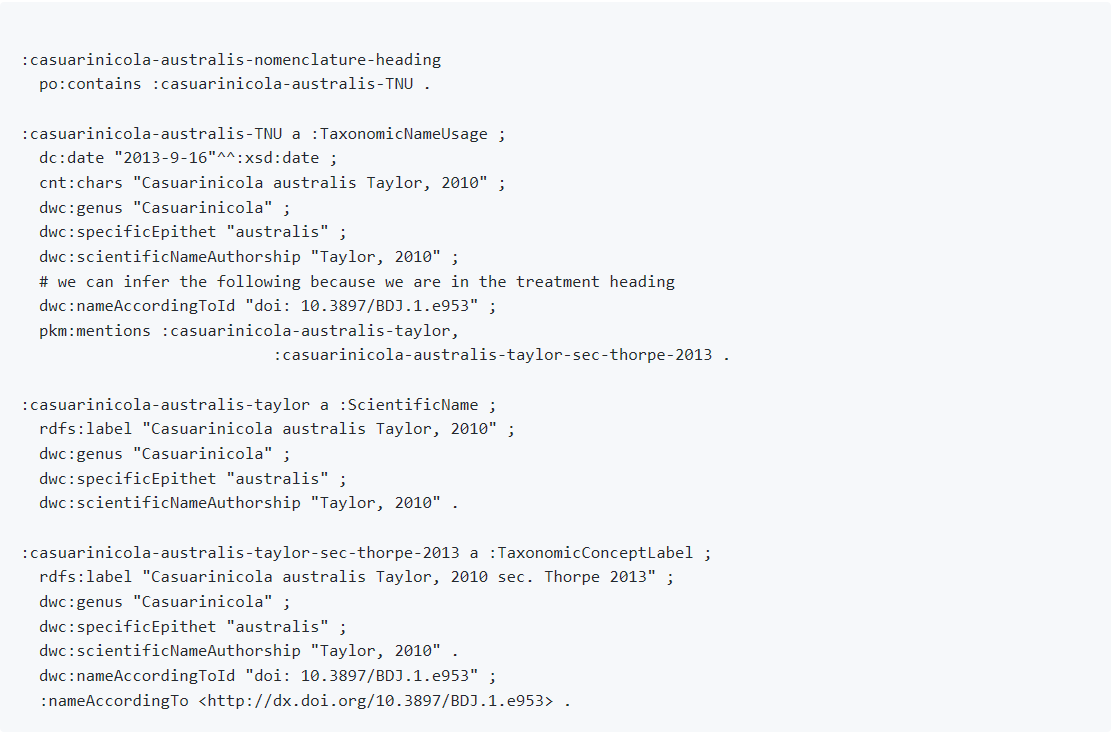
\includegraphics[width=\textwidth]{Figures/example-taxonomic-name-usage}
  \decoRule
  \caption[Example taxonomic name usage.]{
  Тези примери показват как таксономичните имена използват свързващите компоненти на документа.}
  \label{example-taxonomic-name-usage}
\end{figure}

\subsection{Семантично моделиране на таксономичните концепции}

В таксономичните имена на OpenBiodiv-O не са носители на семантична информация за таксоните. Тази задача се изпълнява от нов клас, Taxonomic Concept (\cl{TaxonomicConcept}). Таксономична концепция е теорията, която таксономът формира около таксон посредством научна таксономична публикация. Тя винаги има етикет, състоящ се от таксономичното име и библиографско позоваване на статията, в която името е описано. Въвеждаме и по-общ клас, оперативно таксономично звено (\cl{OperationalTaxonomicUnit}), което може да се използва за всички видове таксономични хипотези, включително такива, които нямат правилен таксономичен етикет . Класовата йерархия е илюстрирана на Фиг.~\ref{taxonomic-concept-diagram}.

\begin{figure}[h!]
\centering
  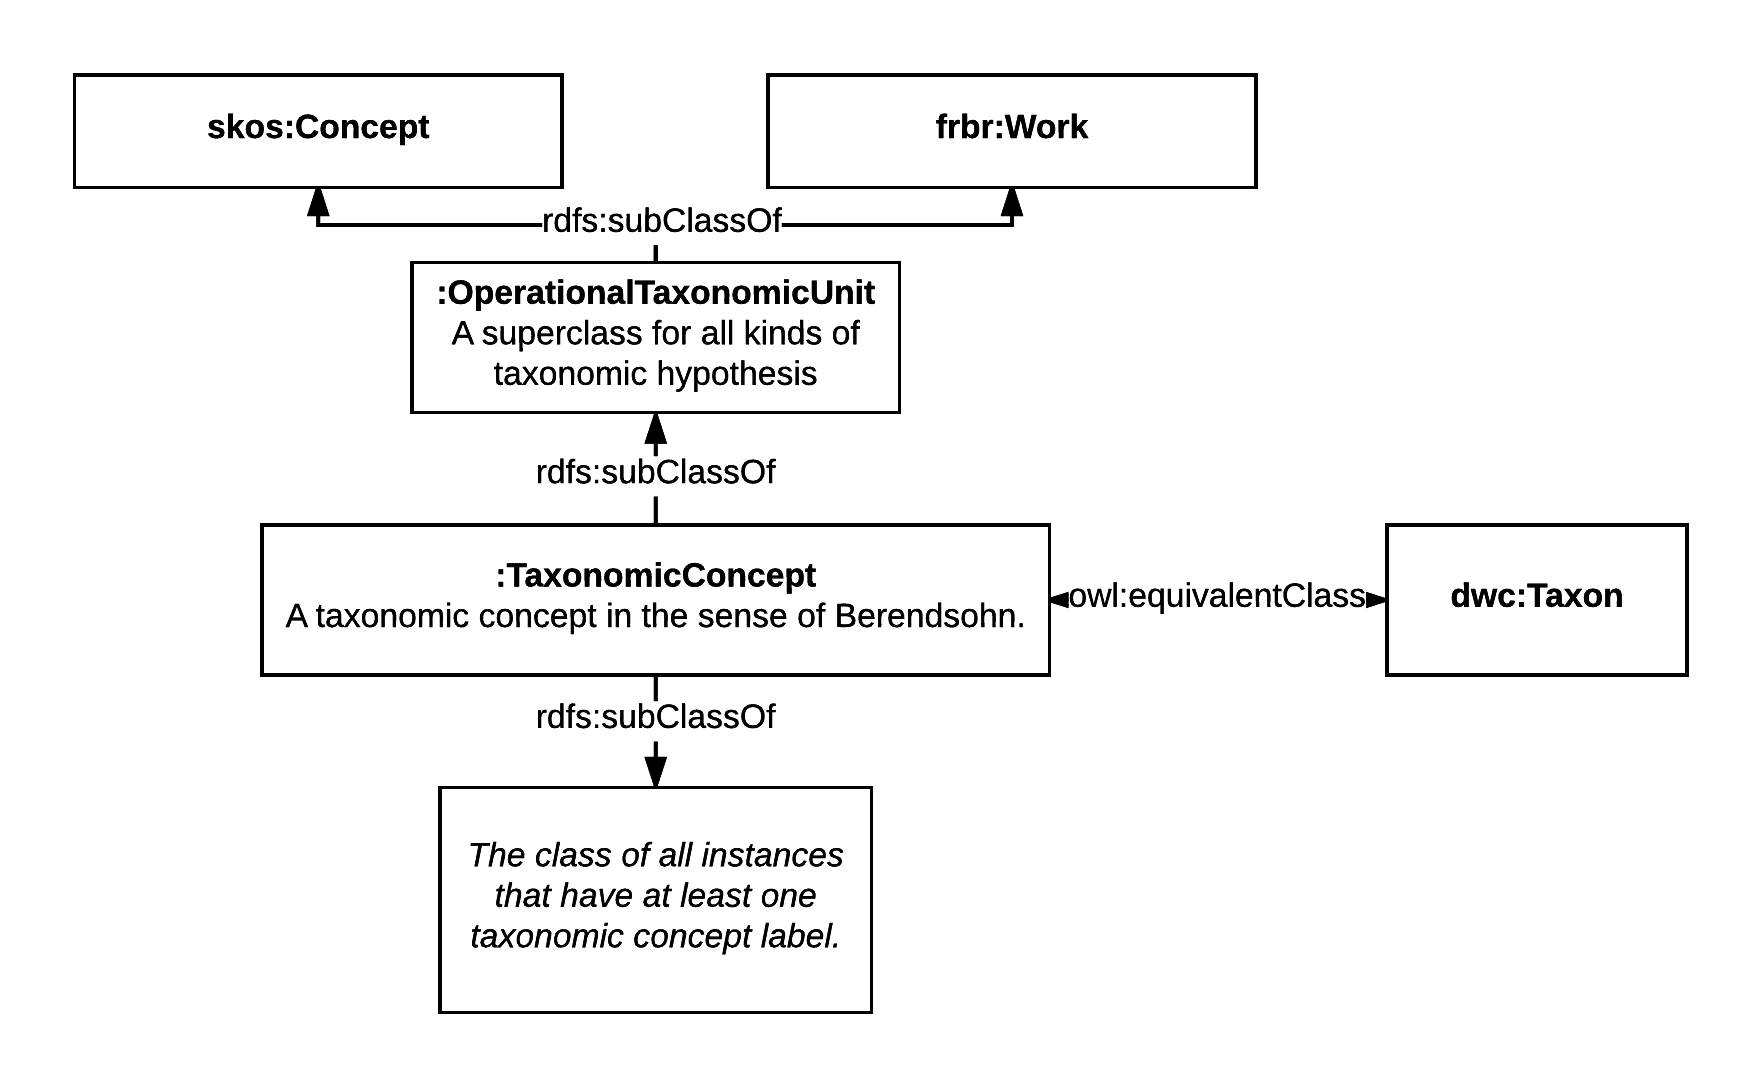
\includegraphics[width=\textwidth]{Figures/taxonomic-concept-diagram}
  \decoRule
  \caption[Taxonomic concept diagram.]{
  Таксономичната концепция е от клас \cl{skos:Concept}, \cl{frbr: Work}, \cl{dwc:Taxon} и има поне един етикет.}
  \label{taxonomic-concept-diagram}
\end{figure}

Свойствата на таксономичните имена са илюстрирани в Фиг.~\ref{name-property-hierarchy}.

\begin{figure}[h!]
\centering
  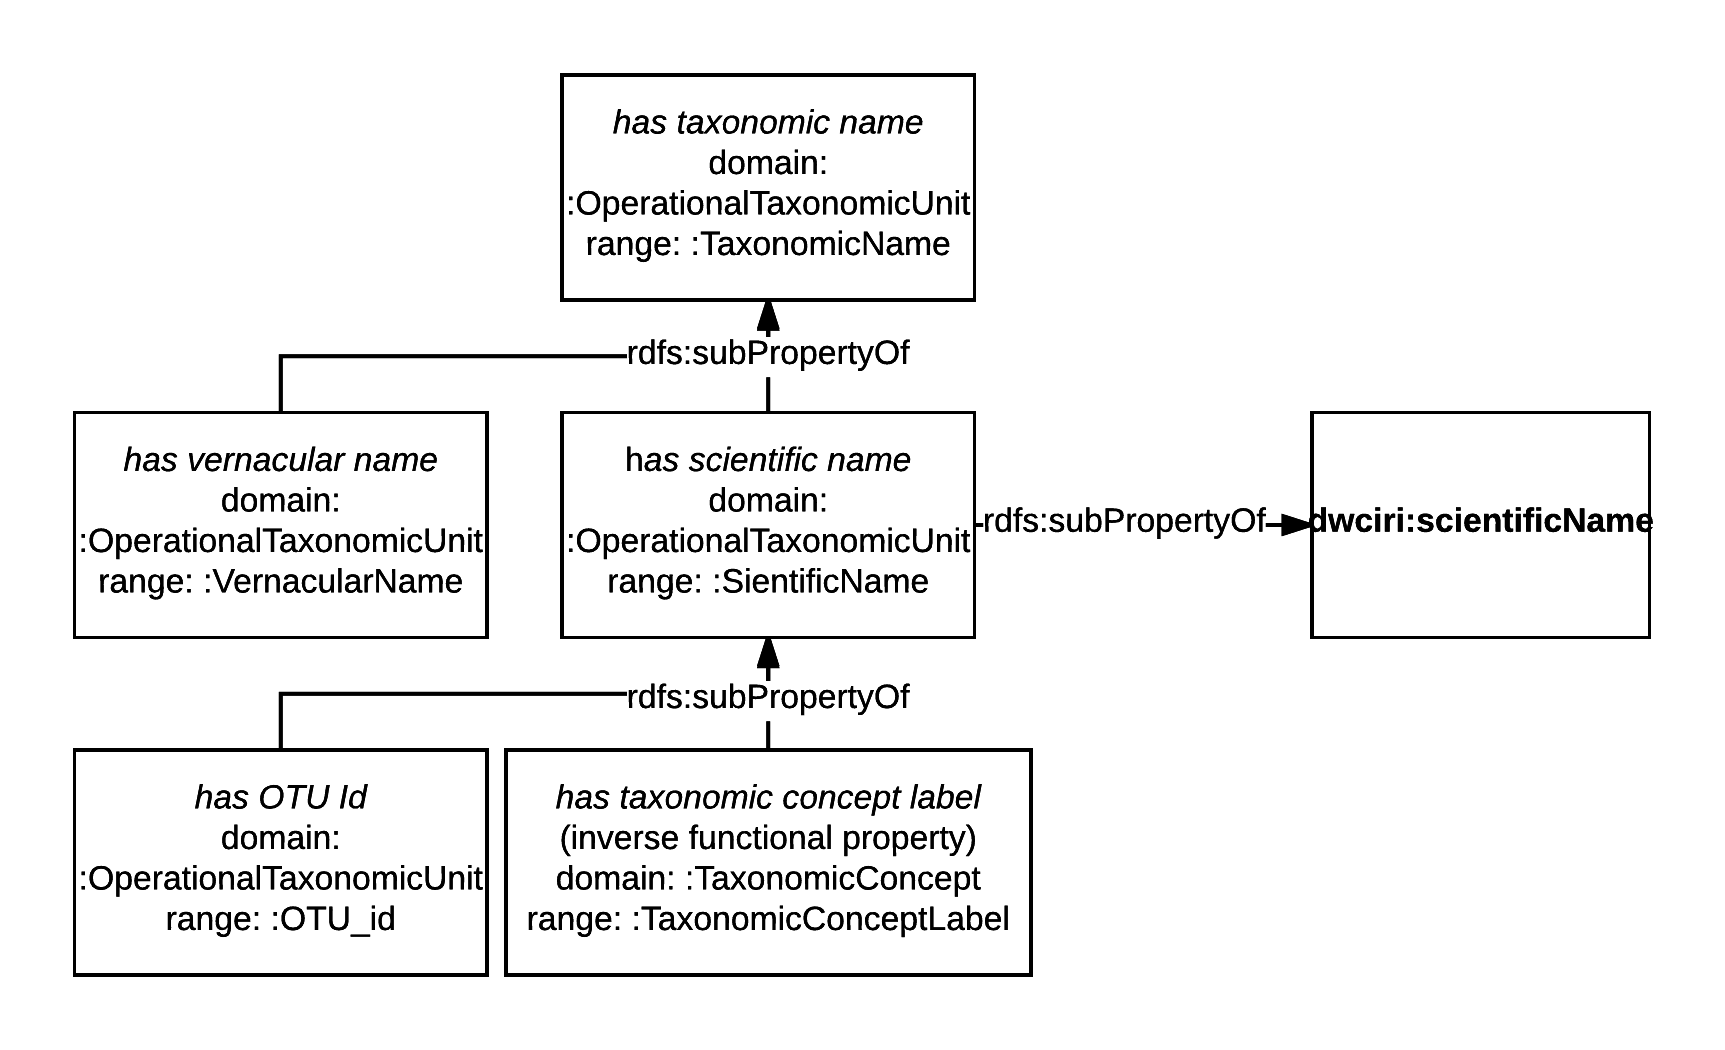
\includegraphics[width=\textwidth]{Figures/name-property-hierarchy}
  \decoRule
  \caption[axonomic name property hierarchy diagram.]
  {Йерархията на свойствата съвпада с йерархията на таксономичните имена и е приравнена към DarwinCore.}
  \label{name-property-hierarchy}
\end{figure}

Двата начина са изразяване на взаимоотношения между таксономични концепции са дадени във Фиг.~\ref{taxonomic-concept-relationships-diagram}).

\begin{figure}[h!]
\centering
  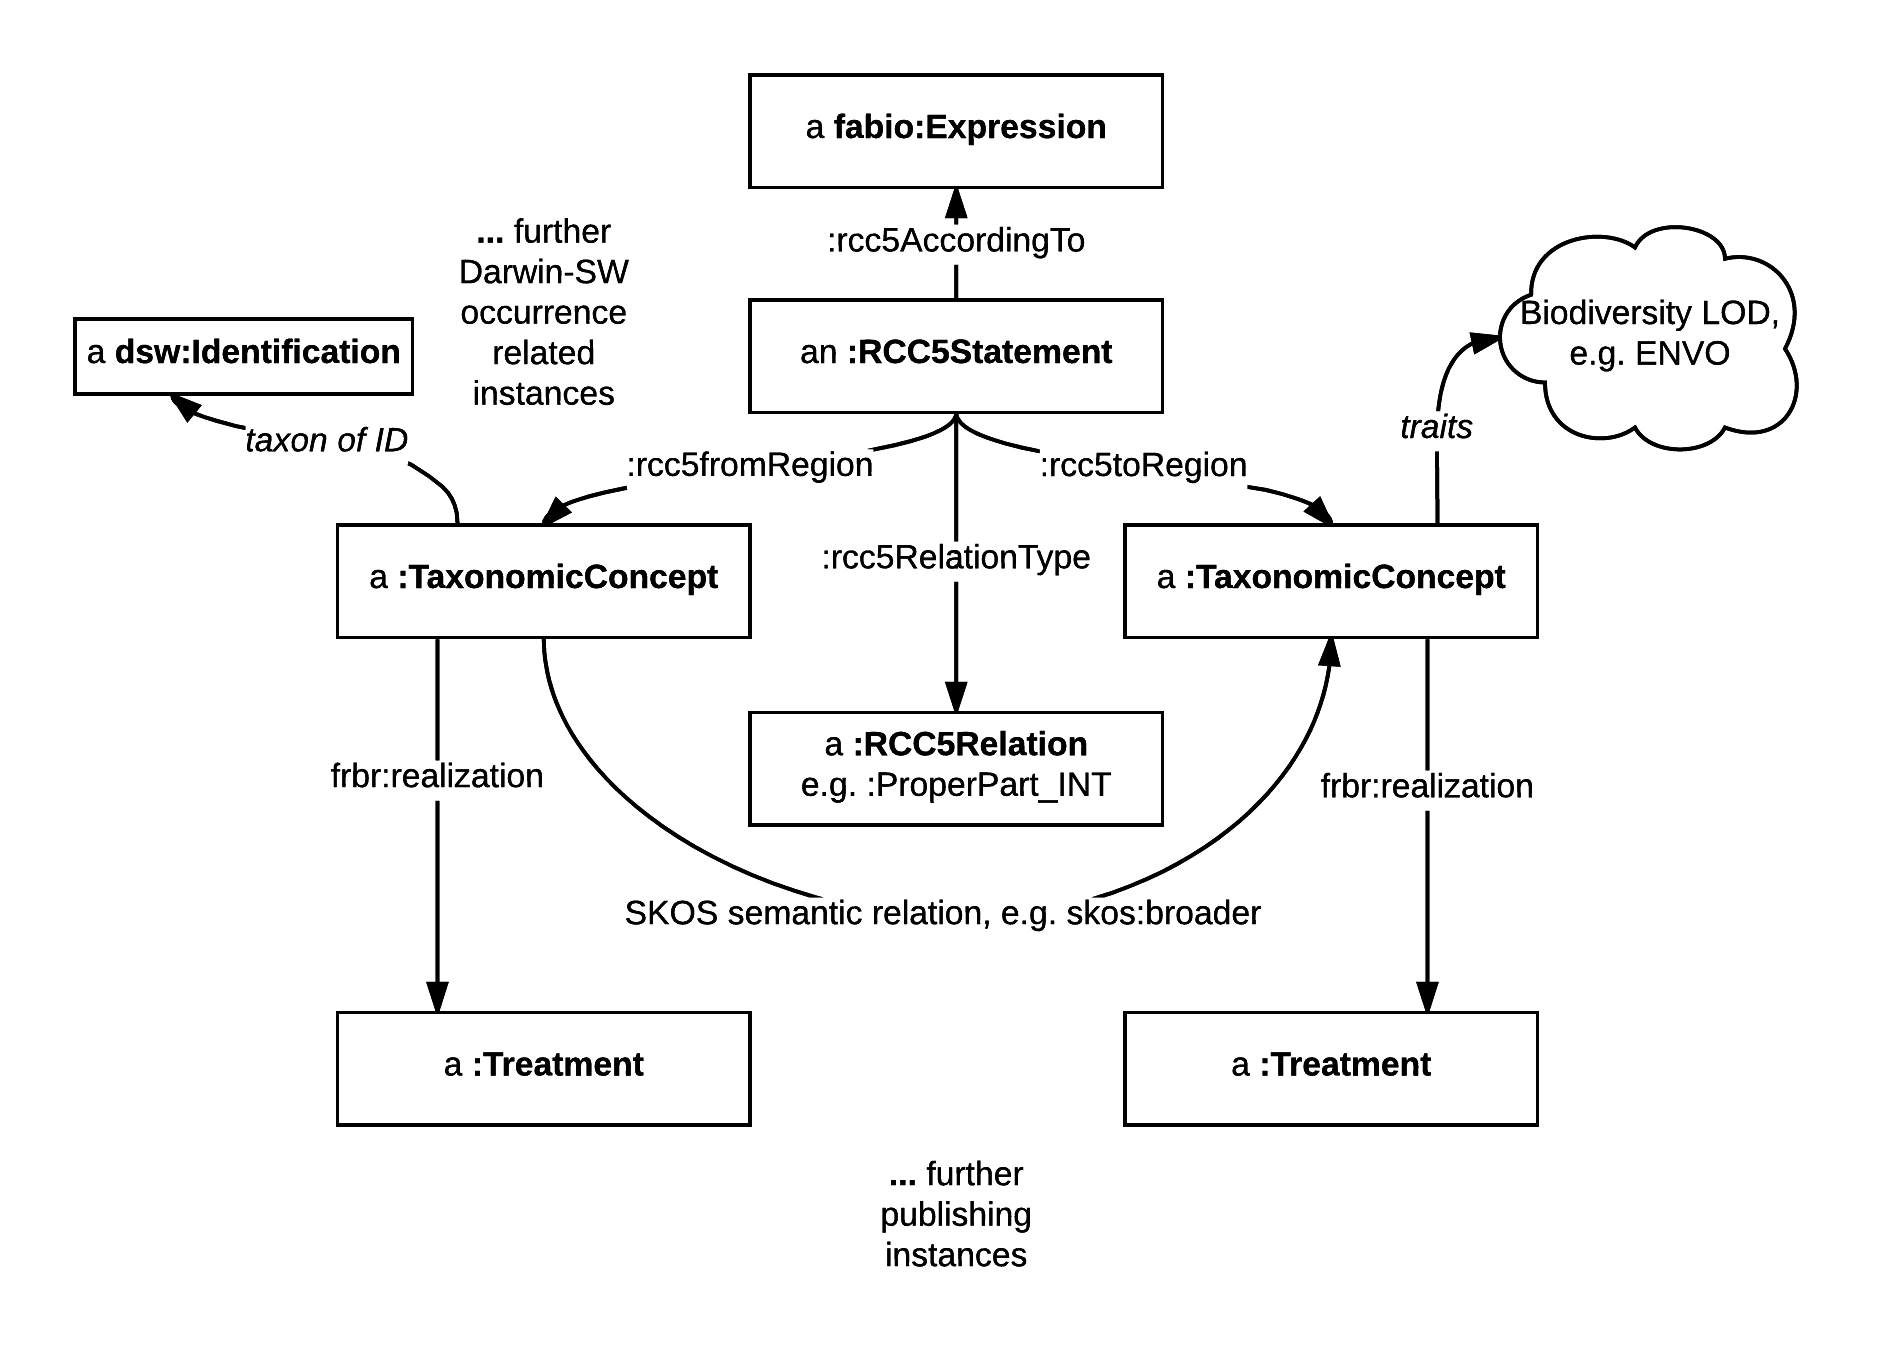
\includegraphics[width=\textwidth]{Figures/taxonomic-concept-relationships-diagram}
  \decoRule
  \caption[Taxonomic concept relationships diagram.]{За да изразите RCC-5 връзка между концепциите, създайте \cl{RCC5Statement} и използвайте съответните свойства, за да свържете две таксономични концепции през него. Освен това, таксономичните понятия са свързани със качества (например екология в ENVO), събития (например Darwin-SW) и са абстрактният клас на Таксономичните дискусии.}
  \label{taxonomic-concept-relationships-diagram}
\end{figure}

Простите отношения не са подходящи за машинен извод. Ето защо \cite{franz_perspectives:_2009}, позовавайки се на \cite{koperski_referenzliste_2000} предложиха да използваме езика RCC-5, за да изразим взаимоотношенията между таксономичните понятия. Тяхни колеги разработиха програмата Euler (\cite{chen_euler/x:_2014}), която използва Answer Set Programming (ASP) за разсъждения и извод по таксономичните взаимоотношения, стъпвайки на RCC-5. Изводната машина за RCC-5 не е част от OpenBiodiv, тъй като тази задача може да бъде изпълнена от Ойлер; въпреки това, ние предоставихме RCC-5 терминилогичен речник. Вж. Фиг.~\ref{example-rcc5-taxonomic-concept-relationships}.

\subsubsection{Семантика и приравняване}

В тази секция таксономичните понятия са приведени в съответствие с DarwinCore (DwC) и е проведена дискусия за това как са представени таксономичните понятия, свързани както с прости отношения (SKOS), така и в подходящ за извод вид (RCC-5). Също така се обсъждат взаимоотношенията между биологичните имена и таксономичните концепции.

\subsubsection{Употреба} Фиг.~ \ref{example-simple-taxonomic-concept-relationships}, Фиг.~\ref{example-rcc5-taxonomic-concept-relationships}, и Фиг.~\ref{example-envo}, и  Fig~\ref{example-treatment-concept}.

\begin{figure}[h!]
\centering
  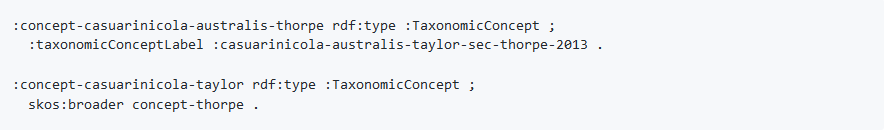
\includegraphics[width=\textwidth]{Figures/example-simple-taxonomic-concept-relationships}
  \decoRule
  \caption[Example simple taxonomic concept relationships.]
  {Можем да използваме семантичните свойства на SKOS, за да илюстрираме прости отношения между таксономичните концепции.}
  \label{example-simple-taxonomic-concept-relationships}
\end{figure}

\begin{figure}[h!]
\centering
  
\includegraphics[width=\textwidth]{Figures/example-rcc5-taxonomic-concept-relationships}
  \decoRule
  \caption[Example of RCC-5 taxonomic concept relationships.]{За да се изрази една RCC-5 връзка между концепциите, създайте \cl{RCC5Sgtatement} и използвайте съответните свойства, за да свържете две таксономични концепции през него.}
  \label{example-rcc5-taxonomic-concept-relationships}
\end{figure}


\begin{figure}[h!]
\centering
  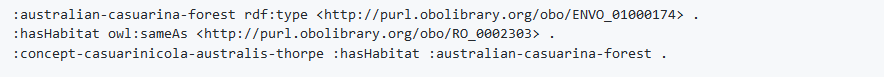
\includegraphics[width=\textwidth]{Figures/example-envo.png}
  \decoRule
  \caption[Example of combining ENVO with OpenBiodiv-O.]{Илюстрация на приравняване към ENVO.}
  \label{example-envo}
\end{figure}



\begin{figure}[h!]
\centering
  
\includegraphics[width=\textwidth]{Figures/example-treatment-concept}
  \decoRule
  \caption[Example connection between a treatment and a taxonomic concept.]{Таксономичната дискусия е реализация/израз/запис на таксономична концепция.}
  \label{example-treatment-concept}
\end{figure}

\section{Дискусия}

Обсъжда се как OpenBiodiv-O е първият по рода си опит да се моделира онтологично таксономичната публикация. Тя проправя пътя към създаване на граф от знания за биологичното разнообразие.

\section{Заключение}

Главата предоставя концептуализация на таксономичния процес и формализация в OpenBiodiv-O. Въвеждат се класове и свойства в областта на публикуването на биоразнообразие и биологичната систематика и ги привежда в съответствие с важните онтологии, специфични за този домейн.
\chapter{Резюме на глава 3: Свързани отворени данни}
\label{chapter-lod}

В глава~\ref{chapter-lod} разглеждаме подробно източниците на данни и техните модели. Създадохме свързани отворени данни OpenBiodiv LOD, съдържащи информация за биологичното разнообразие, извлечена от списанията на Пенсофт, базата данни на Плаци, които е интегрирана с помощта на таксономичния гръбнак на GBIF. Като онтология използваме новия \mbox{OpenBiodiv-O}, разработен в хода на дисертацията. Предлагаме на общността на информатиката за биоразнообразието да използва OpenBiodiv LOD като централна точка на семантичния граф за знания за биоразнообразието. OpenBiodiv LOD е достъпен под \url{http://graph.openbiodiv.net}.

OpenBiodiv LOD е синтетичен набор от данни. Той не съдържа предварително непубликувани данни. Вместо това той интегрира в една база от знания информация, която преди това е била оповестена в академични списания и бази данни. Интеграцията, разбира се, позволява материализацията на скрити взаимоотношения. В следващите няколко параграфа ще обсъдим източниците на информация, които бяха комбинирани от OpenBiodiv LOD и видовете ресурси, които бяха извлечени, както и общия модел на данните. Също така обсъждаме принципите на Linked Open Data, които свързват всичко заедно. Главата завършва с много примери за заявки в набора от данни и с техническа дискусия за начина, по който тя е генерирана.

\section{Източници на данни}

Данните в OpenBiodiv към времето на писането на дисертацията идват от три основни източника: таксономичния гръбнак на GBIF (\cite{gbif_secretariat_gbif_2017}), и научни статии публикувани от Пенсофт, както и съхранявани от Плаци(Fig.~\ref{fig:openbiodiv-sources-simple}).

\begin{figure}
\centering
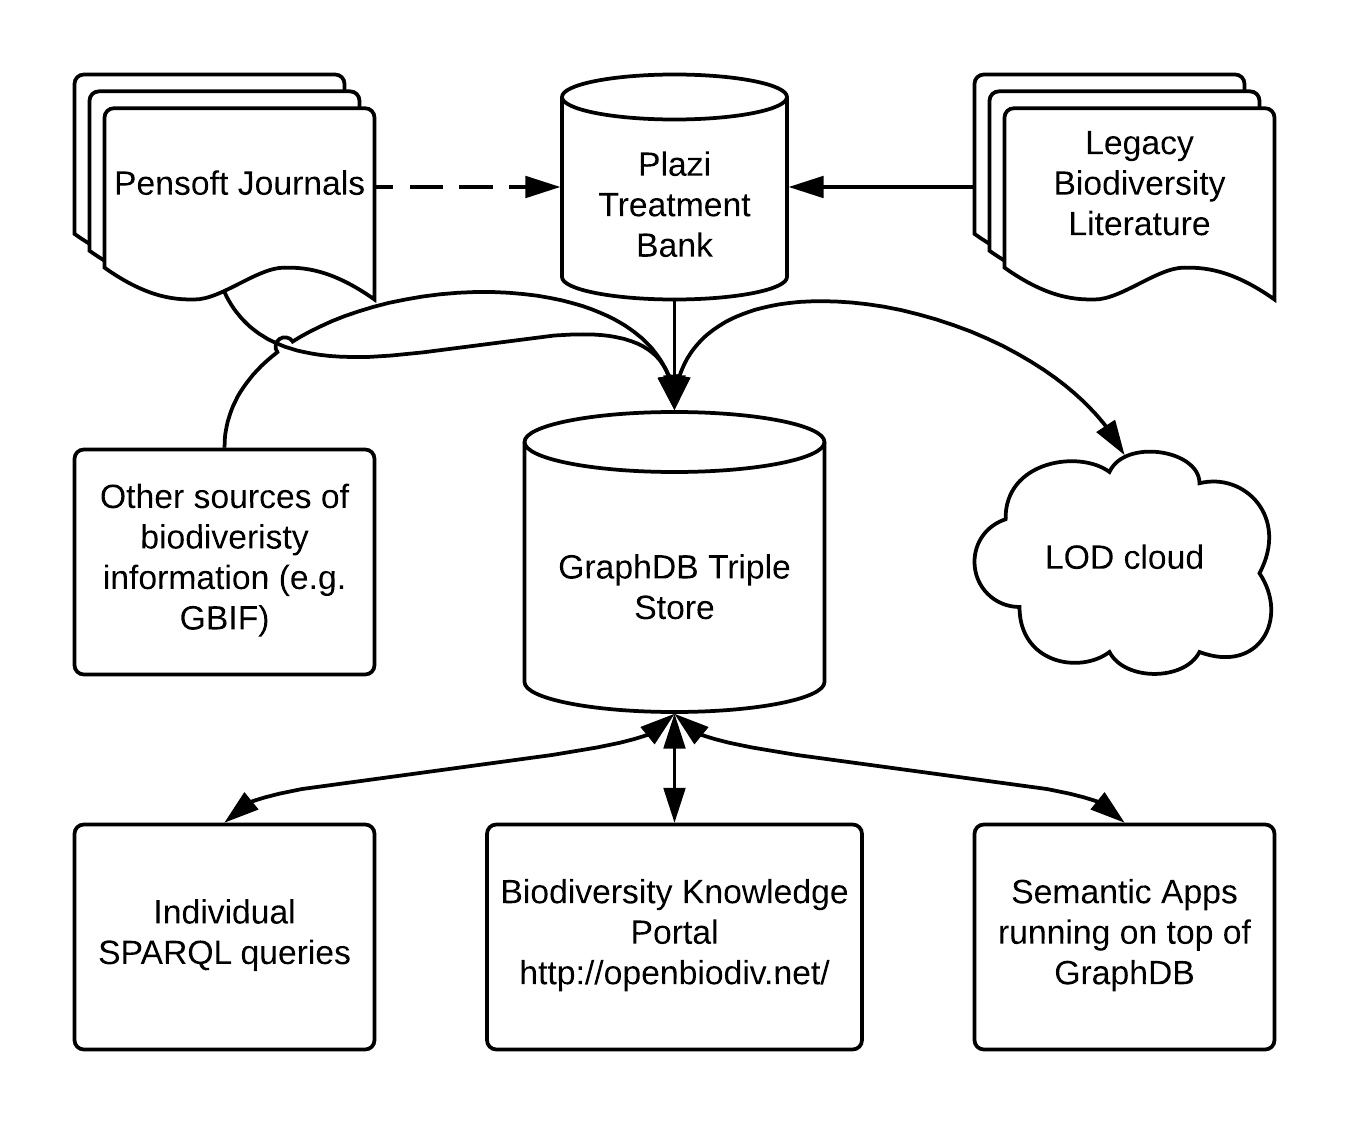
\includegraphics[width=\textwidth]{Figures/openbiodiv-sources-simple}
\decoRule
\caption{Опростен модел на архитектурата на OpenBiodiv от глава~\ref{chapter-openbiodiv} фокусираща върху източниците на информация.}
\label{fig:openbiodiv-sources-simple}
\end{figure}


\subsection{Таксономичен гръбнак на GBIF}

GBIF е най-голямото международно хранилище на данни за наблюдения на организми (occurrence data). GBIF позволява на потребителите да търсят в тяхната система, като използват таксономична йерархия. Например, възможно е да се търсят в базата наблюдения на организми, принадлежащи към определен род: напр. търсене на бръмбар {\textit Harmonia} sec. \cite{gbif_secretariat_gbif_2017} на 30 юни 2018 г. върна 575,376 резултата. Това търсене е възможно благодарение на таксономичния гръбнак на GBIF, Nub (\cite{gbif_secretariat_gbif_2017}). Nub е база данни, която организира таксономични концепции в йерархия, обхващаща всички имена, събрани от GBIF. Тя е синтетична (алгоритмично генерирана) класификация покриваща всички имена, присъстващи в наборите от данни на GBIF. По този начин гръбнакът GBIF не представлява експертен консенсус за това как таксоните са йерархично подредени според еволюционните критерии в природата.

За да предоставим същите възможности на OpenBiodiv, ние  импортирахме Nub като \cl{openbiodiv:TaxonomicConcept} по OpenBiodiv-O (фиг.~\ref {fig:harmonia-halii-visual}).
\begin{figure}
\centering
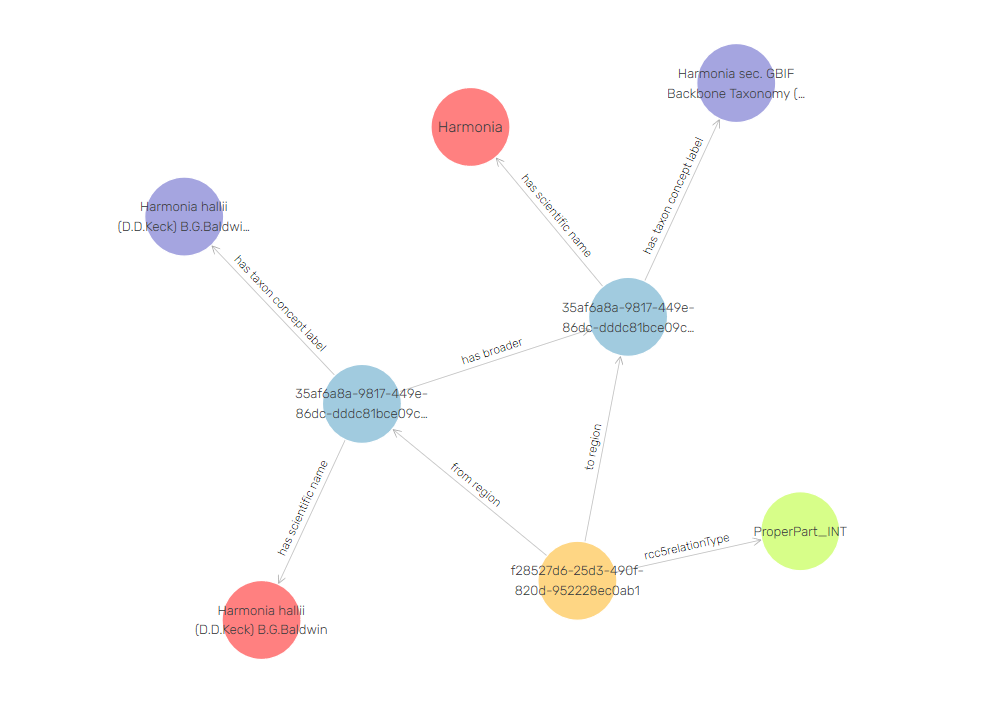
\includegraphics[width=\textwidth]{Figures/harmonia-halii-visgraph}
\decoRule
\caption[Visual graph of \emph{Harmonia halii}]{Илюстрация на представянето на йерархична информаци, импортирана от GBIF като таксономични концепции в OpenBiodiv.}
\label{fig:harmonia-halii-visual}
\end{figure}


\subsection{Пенсфот и Плаци}

Всички валидни статии, от таксономичните списания, публикувани  от Пенсофт и упоменати в Таблица~\ref{rdf-pensoft-journals} бяха конвертирани в RDF и съхранени в гр\'{а}фа от знания на биологичното разнообразие. В допълнение, всички валидни таксономични дискусии (treatments) на Плаци бяха конвертирани в RDF и също съхранени в гр\'{а}фа. Процедурата по RDF-изиране се повтаря всяка седмица и по този начин семантичната база данни винаги съдържа най-новите статии и таксономични дискусии. RDF-изацията е възможнa благодарение на факта, че списанията на Пенсофт публикуват статии в TaxPub XML (\cite{catapano_taxpub:_2010}) докато Плаци публикува дискусиите си в TaxonX (\cite{penev_xml_2011}) (Fig.~\ref{fig:tnu-vis}). И двете схеми са стандартни и общо-достъпни.

\begin{table}[h!]
\caption{Списания ма Пенсофт, които са превърнати в RDF.}
      \begin{tabular}{ccc}
        \hline
          Journal Name             & Submission Style & Number of Articles\\  \hline
          ZooKeys                 & Word document & 3829\\
          PhytoKeys               & Word document & 537\\
          MycoKeys                & Word document & 127\\
          Biodiversity Data Journal & Web based (ARPHA) & 490\\
          Journal of Orthoptera Research & Word document & 32
      \end{tabular}
      \label{rdf-pensoft-journals}
\end{table}

\begin{table}[h!]
\caption{Типове данни, маркирани в TaxPub and TaxonX и тяхната кореспондеция към RDF типовете, които се използват в OpenBiodiv.}
      \begin{tabular}{cccc}
        \hline
          Datatype             & TaxPub & TaxonX & RDF Type\\  \hline
          Article metadata     & T & T & {\tt fabio:JournalArticle} and related\\
          Keyword group        & T & F & {\tt openbiodiv:KeywordGroup} \\
          Abstract             & T & T & {\tt sro:Abstract}\\
          Title                & T & F & {\tt doco:Title} \\
          Author               & T & T & {\tt foaf:Person} \\
          Introduction section & T & F & {\tt deo:Introduction}\\
          Discussion section   & T & T & {\tt orb:Discussion}\\
          Treatment section    & T & T & {\tt openbiodiv:Treatment}\\
          Nomenclature section & T & T & {\tt openbiodiv:NomenclatureSection}\\
          Materials examined   & T & T & {\tt openbiodiv:MaterialsExamined}\\
          Diagnosis section    & T & T & {\tt openbiodiv:DiagnosisSection} \\
          Distribution section & T & T & {\tt openbiodiv:DistributionSection}\\
          Taxonomic key        & T & T & {\tt openbiodiv:TaxonomicKey}\\
          Figure               & T & T & {\tt doco:Figure}\\
          Taxonomic name usage & T & T & {\tt openbiodiv:TaxonomicNameUsage}
      \end{tabular}
      \label{datatypes-taxpub-taxonx}
\end{table}

\begin{figure}
\centering
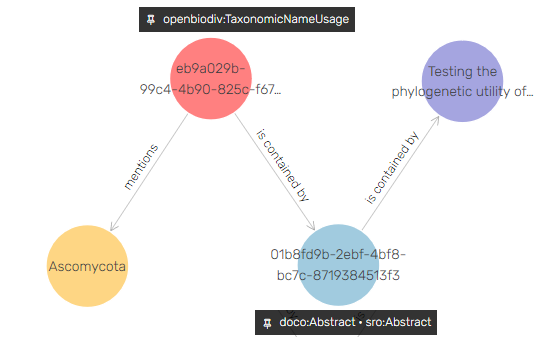
\includegraphics[width=\textwidth]{Figures/tnu-vis}
\decoRule
\caption[Visual graph of a taxonomic name usage]{Употреба на таксономични имена в OpenBiodiv (taxonomic name usage).}
\label{fig:tnu-vis}
\end{figure}

\section{Свързани отворени данни}

Linked Open Data (LOD, \cite{heath_linked_2011}) е идея на Семантичната Мрежа (\cite{berners-lee_semantic_2001}) целяща да гарантира полезността на данни публикувани в Мрежата, като улеснява тяхното повторно намиране и употреба от трети лица. В тази секция разясняваме принципите на Свързаните Отворени Данни и тяхното приложение в OpenBiodiv (\cite{heath_linked_2011}).

\begin{figure}
\centering
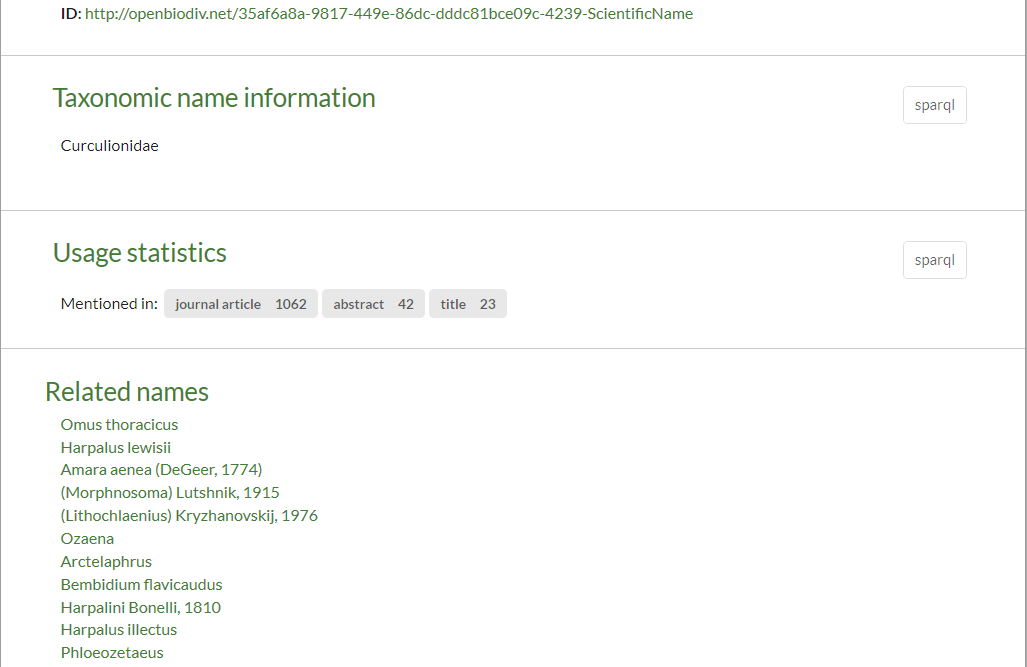
\includegraphics[width=\textwidth]{Figures/portal-name-visualization}
\decoRule
\caption{Визуализация.}
\label{fig:portal-name-visualization}
\end{figure}


\section{Модел на данните}

Подчертаваме, че използваме модела подробно разяснен в глава~\ref{chapter-ontology} и допълнителните онтологии (Fig.~\ref{fig:community-ontologies}).

\begin{figure}
\centering
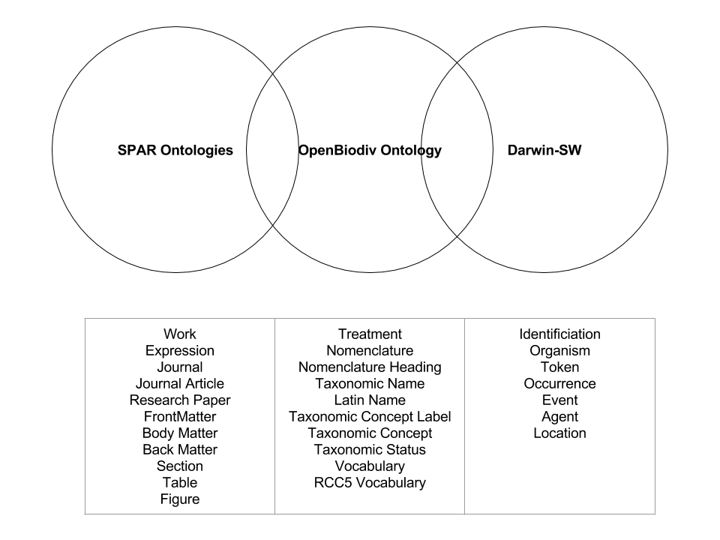
\includegraphics[width=\textwidth]{Figures/community-ontologies}
\decoRule
\caption[Overlap of OpenBiodiv-O with Community Ontologies]{Връзка между OpenBiodiv-O и други публично-достъпни онтологии.}
\label{fig:community-ontologies}
\end{figure}

\section{Примерен SPARQL}

В тази секция илюстрираме, как представеният модел за данни, заедно с инкорпорираната в базата данни информация е достатъчен за да изпълним някои много интересни заявки върху графа за знания.

\subsection{Прости заявки}

В тази подскекция даваме прости заявки. Напр. как да търсим по автори, по научни имена и т.н.

\subsubsection{Заявка върху структурата на статията} 

Тъй като в OpenBiodiv LOD статиите са разбити по техните компоненти (вж напр. Таблица~\ref{datatypes-taxpub-taxonx}) и споменаванията на таксони (taxonomic name usages) винаги са свързани със специфична част на статията, може да правим запитвания, използващи тази структура.

\subsubsection{Запитване за таксономични концепции}

Дадени са пример за SPARQL заявки, базиращи се на таксономични концепции.

\subsubsection{Размито търсене с Lucene}

Използваме Lucene connector (\cite{ontotext_graphdb_2018}) на GraphDB, за да допълним точните търсения с размити търсения, където се допускат правописни грешки.

\subsection{Отговаряне на експертни въпроси}

Поради машината си за извод, OpenBiodiv може да функционира като експертна система. В тази подсекция даваме примери за такова запитване.

\subsubsection{Проверка на валидността на таксономично име}

Проверяваме, дали дадено таксономично име е валидно, т.е. е уместно да се употребява в научен контекст, или е било прехамахнато или заменено от друго име.

\subsubsection{Оценка на научната загуба след пожара в Museu Nacional в Бразилия}

Може да запитаме експертната система OpenBiodiv да даде списък с видовете, чиито екземпляри бяха загубени в пожара в Рио де Жанейро.

\section{Как създадохме данните?}

В тази секция се разкриват техническите подробности за това, как данните бяха създадени.

\subsection{Получаване на данни}

Дават се адресите в Интернет, където данните в суров вид могат да бъдат достъпвани.

\subsection{Инструменти}

Използват се следните инструменти

\begin{enumerate}
\item{Пакет RDF4R}
\item{Пакет ROpenBio}
\item{Пакет TSV4RDF разработен от Пенсофт}
\item{Базисен код на OpenBiodiv}
\end{enumerate}

\subsection{Трансформация от XML в RDF}

Използваме йерархичната структура на XML, за да решим проблема рекурсивно с помощта на следния Extractor, документиран в Алгоритъм~\ref{algo:extractor}.

% http://tug.ctan.org/macros/latex/contrib/algorithmicx/algorithmicx.pdf
\begin{algorithm}
\caption{Екстрактор}
\begin{algorithmic}[1]
\Procedure {Extractor}{XML Node $X$}
\State $a \leftarrow$ extract atoms of $X$
\Comment Atoms extraction
\State $r \leftarrow$ construct RDF from $a$
\Comment RDF construction
\State $C \leftarrow$ find relevant sub-nodes of $X$
\Comment Recursively applies itself
\State $R \leftarrow$ apply Extractor on each $C_i \in C$
\State \Return $r \bigcup R$
\EndProcedure
\end{algorithmic}
\label{algo:extractor}
\end{algorithm}

\subsubsection{Извличане на атомите}

Текстовите полета в XML ще наричаме атоми. Тяхното извличане се осъществява с помощта на езика XPATH. Тук разясняваме, как става това.

\subsubsection{Генериране на RDF}

След извичане на атомите, те могат да бъдат събрани обратно във формата на RDF. 

\subsubsection{Стратегия разделяй и владей}

Проблемът за RDF-изиранато на цял XML файл е реализиран посредством разбиването му на малки проблеми, за които решението е тривиално като в горния пример за RDF-изирането на даден автор или на метаданните на дадена статия.

\subsubsection{Дефиниране на трансформацията}

За да работи Extractor, трябва да дефинираме XML схемата. Спецификацията включва какви XML възли търсим и къде се намират. След това рекурсивно се указва за всеки възел кои под-възли търсим и тяхното местоположение на XPATH спрямо техния родителски възел. И накрая, за всеки възел трябва да дадем атомните места и да напишем конструктор. Спецификацията на трансформацията се извършва в R6 калс на R. Определихме две схеми, които споделят същите конструктори: TaxPub\footnote{\url{https://github.com/pensoft/ropenbio/blob/redesign/R/taxpub.R}} и TaxonX\footnote{\url{https://github.com/pensoft/ropenbio/blob/redesign/R/taxonx.R}}.

\subsection{Качване в базата данни и допълнителна обработка}

Извлечените RDF твърдения се изпращат в GraphDB, който се намира на адрес \url{http://graph.openbiodiv.net/}. Освен материлизирани твърдения по онтологията, след всеки ъпдейт, изпълняваме следните допълни правила: 

\subsubsection{Ъпдейт на заместващите имена}

Изгражда връзките от тип \cl{replacementName} между вмъкнатите имена.

\section{Дискусия}

Установихме, че обемът данни, който обработване в комбинация с пълна OWL логика води до неприемлива производителност. В тази секция разглеждаме този проблем (Фиг.~\ref{fig:statements-report}).

\begin{figure}
\centering
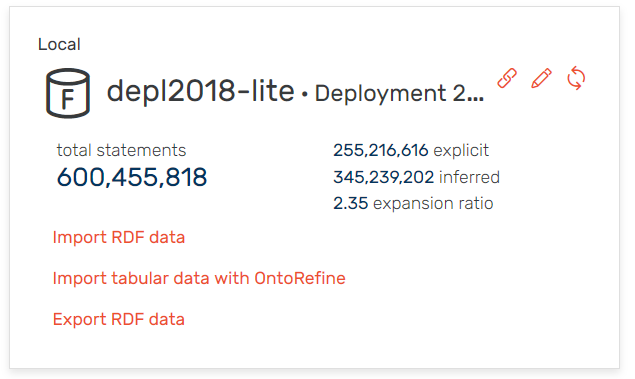
\includegraphics[width=\textwidth]{Figures/active-repository}
\decoRule
\caption[Statements report]{Брой твърдения.}
\label{fig:statements-report}
\end{figure}

\begin{figure}
\centering
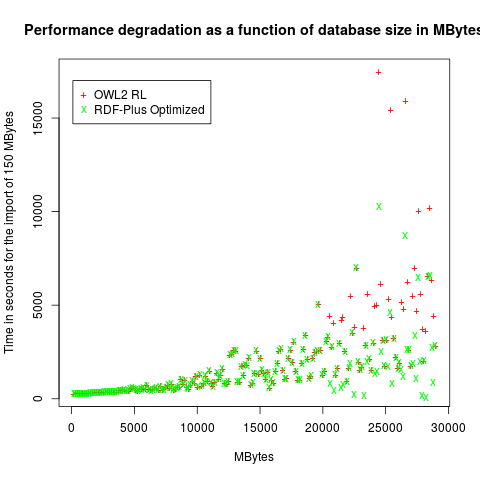
\includegraphics[width=\textwidth]{Figures/performance-degradation-both}
\decoRule
\caption[Performance degradation]{Визуализация на деградацията на производителността.}
\label{fig:performance-degradation}
\end{figure}

Правим някои основни изводи и очертаваме насоки за бъдещо развитие.
\chapter{Summary of Chapter 4: An R Library for Working with RDF}
\label{chapter-rdf4r}

RDF4R ({\tt rdf4r}) is an R package for working with Resource Description Framework (\cite{rdf_working_group_resource_2014}) data. It was developed as part of the OpenBiodiv project but is completely free of any OpenBiodiv-specific code and can be used for generic purposes requiring tools to work with RDF data in the R programming environment (\cite{r_core_team_r:_2016}).

\section{Installation}

In this section we describe how to install the RDF4R package. Installation is straighforward and consists of two steps: (1) resolve dependencies and (2) build the package from source using \cl{devtools::install_github}.

\section{Specification}

In this section we present the specifications of RDF4R by detailing the features of the package. Each feature has a dedicated subsection.

\subsection{Connection to a triple-store}

It is possible to establish both basic connections (requiring no password or requiring basic HTTP user-pass authentication) or connection secured with an API access token.

\subsection{Work with repositories on a triple-store}

Once a connection to a triple-store has been established, it is possible to inspect the talk protocol version, view the list of repositories on the database, execute SPARQL Read (SELECT keyword and related) and SPARQL Update (INSERT and related) queries on the database, as well as submit serialized RDF data directly to the database.

\subsection{Function factories to convert SPARQL queries to R functions}

An important feature of RDF4R are its facilities for converting SPARQL queries and the like to R functions.

\subsection{Work with literals and identifiers}

The building blocks of RDF are literals (e.g. strings, numbers, dates, etc.) and resource identifiers. RDF4R provides classes for literals and resource identifiers that are tightly integrated with the other facilities of the package.

\subsection{Prefix management}

Prefixes are managed automatically during serialization by being extracted from the resource identifiers.

\subsection{Creation and serialization of RDF}

The serialization function supports Turtle (and its variant Trig, \cite{bizer_rdf_2014}) and adding new triples.

\begin{lstlisting}[language=SPARQL,
caption=Using brackets to express RDF blank nodes in Turtle/TriG.,
label=fig:turtle-brackets,
basicstyle=\ttfamily\tiny]
@prefix foaf: <http://xmlns.com/foaf/0.1/> .

# :someone knows someone else, who has the name "Bob".
:someone foaf:knows [ foaf:name "Bob" ] .
\end{lstlisting}

\subsection{A basic vocabulary of semantic elements}

RDF4R has some basic resource identifiers for widely used classes and predicates predefined (e.g. for {\tt rdf:type}, {\tt rdfs:label}, etc.).

\section{Usage}

Here, we explain how to use the package RDF4R by means of examples. In order to fully utilize the package capabilities, one needs to have access to an RDF graph database. We have made available a public endpoint (see next paragraph) to allow the users of the package to experiment. Since write access is enabled, please be considerate and don't issue catastrophic commands.

\section{Discussion}

\subsection{Related Packages}

The closest match to RDF4R is the {\tt rdflib} (\cite{boettiger_rdflib:_2018}). The development of the two packages was simultaneous and independent until {\tt rdflib}'s first official release on Dec 10, 2017. This explains why two closely related R packages for working with RDF exist. After the release of {\tt rdflib} work was started  to make both packages compatible with each other. In our opinion, the packages have different design philosophies and are thus complementary.

{\tt rdflib} is a high-level wrapper to {\tt redland} (\cite{jones_redland:_2016}), which is a low-level wrapper to the C {\tt librdf} (\cite{beckett_redland_2014}), a powerful C library that provides support for RDF. {\tt librdf} provides an in-memory storage model for RDF beyond what is available in RDF4R and also persistent storage working with a number of databases. It enables the user to query RDF objects with SPARQL. Thus, {\tt librdf} can be considered a complete graph database implementation in C.

In our opinion, {\tt redland} is more complex than needed for the purposes of OpenBiodiv. By the onset of the OpenBiodiv project it was available\footnote{But not {\tt rdflib}!}; however, we decided not to use it as a decision was made to rely on GraphDB for our storage and querying. Note that RDF4R's main purpose is to provide a convenient R interface for users of GraphDB and similar RDF4J compatible graph databases.

A feature that differentiates {\tt rdflib} from RDF4R is the design philosophy. RDF4R was designed primarily with the Turtle and TriG serializations in mind. This means that RDF4R can work with named graphs, whereas their usage is discouraged or perhaps impossible with {\tt rdflib}\footnote{The issue was discussed on the {\tt librdf} GitHub page, \url{https://github.com/ropensci/rdflib/issues/23}.}, even though {\tt rdflib}'s default format is N-Quads.

Another differentiating feature between RDF4R and {\tt rdflib} is that RDF4R provides facilities for converting SPARQL and related statements to native R functions!

In a future release of RDF4R (2.0) we would like to replace or extend its in-memory model with {\tt rdflib}'s. This is why we would like to make the packages fully compatible and have contributed several patches to {\tt rdflib}\footnote{Please, consult the commit history under \url{https://github.com/ropensci/rdflib}.}). Thus, it will be possible for the user of RDF4R to retain its syntax and high-level features--- constructor factories, functors, etc., and the ability to use named graphs---but benefit from performance increases, stability, and scalability with the {\tt redland/rdflib/librdf} backend.

This will enable the users of the R programming environment to use whichever syntax they prefer and benefit from an efficient storage engine.

\subsection{Elements of Functional Programming (FP)}

In this subsection we discuss how patterns from functional programming were used to create RDF4R.

\subsection{Elements of Object-Oriented Programming (OOP)}

In this subsection we discuss how patterns from object-oriented programming were used to create RDF4R.

\chapter{Summary of Chapter 5: Workflows for Biodiversity Data}
\label{chapter-case-study}

In this chapter we discuss two automated workflows for exchange of biodiversity data developed as part of OpenBiodiv: (1) automatic import of specimen records into manuscripts, and (2) automatic generation of data paper manuscripts from Ecological Metadata Language (EML) metadata. The workflows were presented at a webinar for the orgnization iDigBio\footnote{Integrated Digitized Biocollections (iDigBio) is a US-based aggregator of biocollections data. They hold regular webinars and workshops aimed at improving biodiversity informatics knowledge, which are attended by collection managers, scientists, and IT personnel. Thus, doing a presentation for iDigBio was an excellent way of making the research and tools-development efforts of OpenBiodiv widely known and getting feedback from the community.} and published as a paper (\cite{senderov_online_2016}).

The slides from the presentation as well as a PDF of the paper are available from the webinar GitHub page under \url{https://github.com/vsenderov/idigbio-webinar}.

\section{Introduction}

Information on occurrences of species and information on the specimens that are evidence for these occurrences (specimen records) is stored in different biodiversity databases. These databases expose the information via public REST API's. I focused on the Global Biodiversity Information Facility (GBIF), Barcode of Life Data Systems (BOLD), iDigBio, and PlutoF, and utilized their API's to import occurrence or specimen records directly into a manuscript edited in the ARPHA Writing Tool (AWT).

Furthermore, major ecological and biological databases around the world provide information about their datasets in the form of EML. A workflow was developed for creating data paper manuscripts in AWT from EML files. Such files could be downloaded, for example, from GBIF, DataONE, or the Long-Term Ecological Research Network (LTER Network).

The development of these workflows focuses on two areas: optimizing the workflow of specimen data and optimizing the workflow of dataset metadata. These efforts resulted in the functionality that it is now possible, via a record identifier, to directly import specimen record information from the Global Biodiversity Information Facility (GBIF), Barcode of Life Data Systems (BOLD), iDigBio, or PlutoF into manuscripts in the ARPHA Writing Tool (AWT). No manual copying or retyping is required. 

\section{Presentation}

A video recording of the presentation is available\footnote{\url{http://idigbio.adobeconnect.com/p7sg0aym3e3/}}. More information can be found in the webinar information page\footnote{\url{http://www.idigbio.org/content/online-direct-import-specimen-records-idigbio-infrastructure-taxonomic-manuscripts}}. The slides of the presentation are attached as supplementary files and are deposited in Slideshare\footnote{\url{http://www.slideshare.net/ViktorSenderov/online-direct-import-of-specimen-records-from-idigbio-infrastructure-into-taxonomic-manuscripts}}.

During the presentation we conducted a poll about the occupation of the attendees, the results of which are summarized in Fig.~\ref{fig:webinar-poll}. Of the participants who voted, about a half were scientists, mostly biologists, while the remainder were distributed across IT specialists and librarians, with 20\% "Other." The other categories might have been administrators, decision-makers, non-biology scientists, collections personnel, educators, etc.

\begin{figure}
\centering
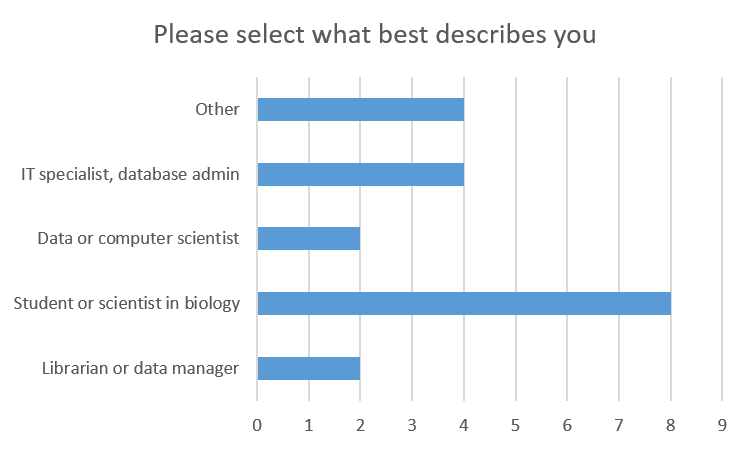
\includegraphics[width=\textwidth]{Figures/webinar-pool}
\decoRule
\caption{Poll results about composition of audience during live participation..}
\label{fig:webinar-poll}
\end{figure}

At the end of the presentation, very interesting questions were raised and discussed. For details, see the ``Results and discussion'' section of this paper.

\section{Methods}

Both workflows discussed  rely on three key standards: RESTful API's for the web (\cite{kurtz_what_2013}), Darwin Core (\cite{wieczorek_darwin_2012}), and EML (\cite{fegraus_maximizing_2005}).

\subsection{Development of workflow 1: Automated specimen record import}

In this subsection we discuss the development of Workflow 1: Automated specimen record import.

\subsection{Development of workflow 2: Automated data paper generation}

In this subsection we discuss the development of Workflow 1: Automated specimen record import.

\section{Results and Discussion}

\subsection{Workflow 1: Automated specimen record import into manuscripts developed in the ARPHA Writing Tool}

It is now possible to directly import a specimen record as a material citation in an ARPHA Taxonomic Paper from GBIF, BOLD, iDigBio, and PlutoF (Slide 5, as well as Fig.~\ref{fig:workflow-idigbio}). The workflow from the user's perspective has been thoroughly described in a blog post; concise stepwise instructions are available via ARPHA's Tips and tricks guidelines. In a nutshell, the process works as follows:

\begin{enumerate}
\item{At one of the supported data portals (BOLD, GBIF, iDigBio, PlutoF), the author locates the specimen record he/she wants to import into the Materials section of a Taxon treatment (available in the Taxonomic Paper manuscript template).}
\item{Depending on the portal, the user finds either the occurrence identfier of the specimen, or a database record identifier of the specimen record, and copies that into the respective upload field of the ARPHA system (Fig.~\ref{fig:occurrence-input-mask}).}
\item{After the user clicks on ``Add,'' a progress bar is displayed, while the specimens are being uploaded as material citations.}
\item{The new material citations are rendered in both human- and machine-readable DwC format in the Materials section of the respective Taxon treatment and can be further edited in AWT, or downloaded from there as a CSV file.}
\end{enumerate}

\begin{figure}
\centering
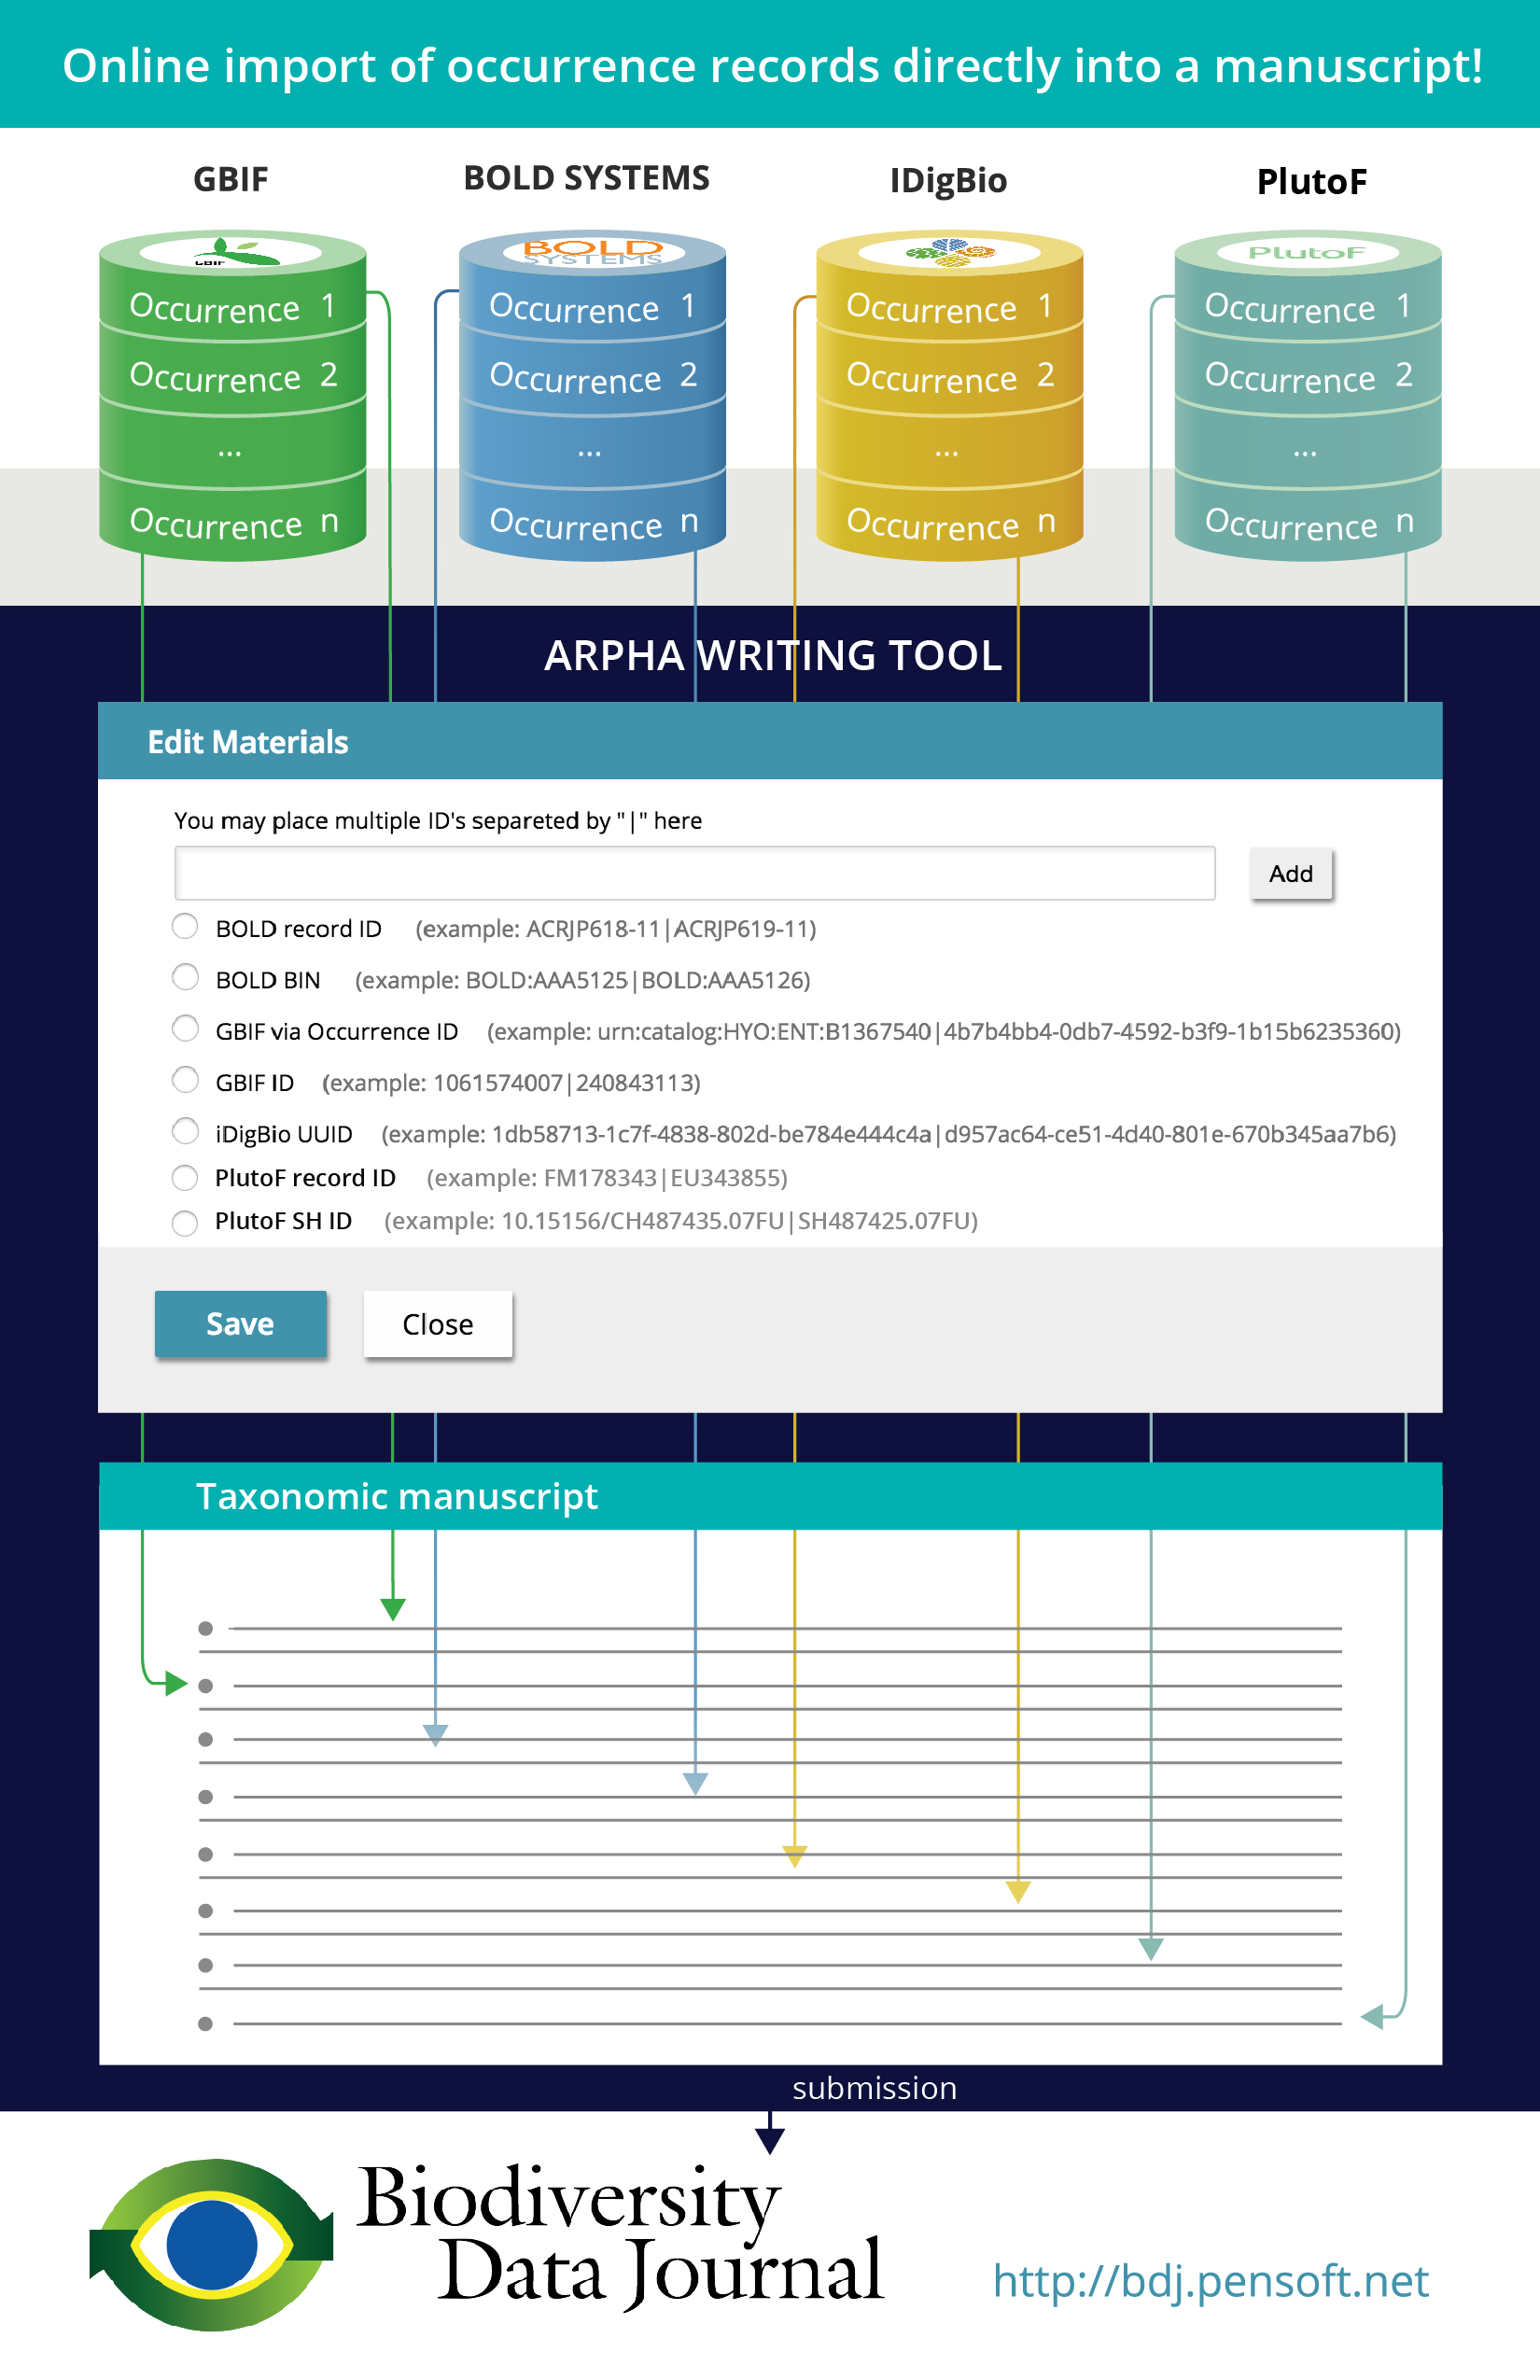
\includegraphics[width=\textwidth]{Figures/workflow-idigbio}
\decoRule
\caption{This fictionalized workflow presents the flow of information content of biodiversity specimens or biodiversity occurrences from the data portals GBIF, BOLD Systems, iDigBio, and PlutoF, through user-interface elements in AWT to textualized content in a Taxonomic Paper manuscript template intended for publication in the Biodiversity Data Journal.}
\label{fig:workflow-idigbio}
\end{figure}

\begin{figure}
\centering
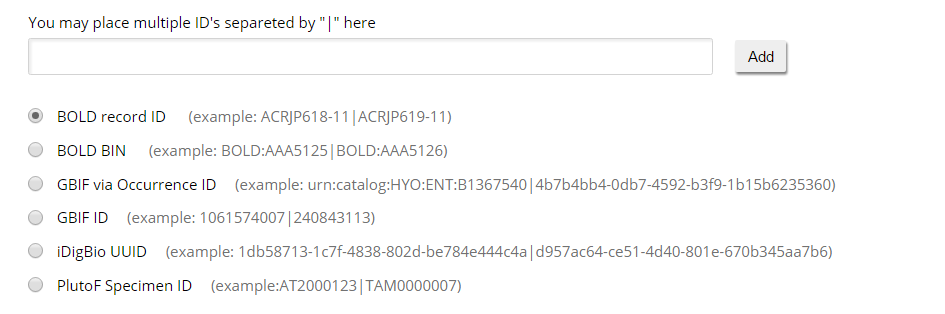
\includegraphics[width=\textwidth]{Figures/occurrence-input-mask}
\decoRule
\caption{User interface of the ARPHA Writing Tool controlling the import of specimen records from external databases.}
\label{fig:occurrence-input-mask}
\end{figure}

\subsubsection{Discussion}

We discuss the availability, or more correctly the lack of persistent unique identifiers (PID's) in the biodiversity informatics space. I furthermore discuss the challenges of importing from our different sources: GBIF, PlutoF, iDigBio, and BOLD. I emphasize how our workflow can be serve as  a curation filter for increasing the quality of specimen data via the scientific peer review process. 

\subsection{Workflow 2: Automated data paper manuscript generation from EML metadata in the ARPHA Writing Tool}

We have created a workflow that allows authors to automatically create data paper manuscripts from the metadata stored in EML (Fig.~\ref{fig:EML-download}, Fig.~\ref{fig:journal-selection}, Fig.~\ref{fig:user-interface}).

\begin{figure}
\centering
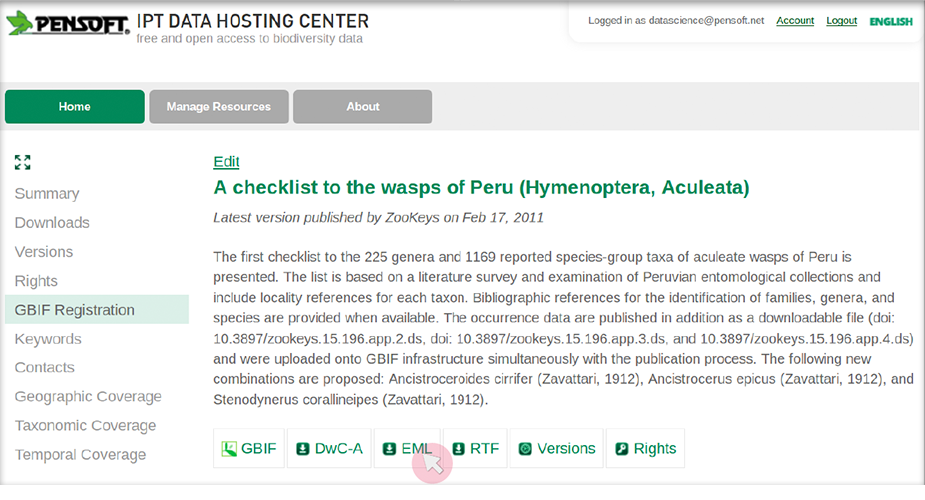
\includegraphics[width=\textwidth]{Figures/EML-download}
\decoRule
\caption{Download of an EML from the GBIF Integarted Publishuing Toolkit (IPT).}
\label{fig:EML-download}
\end{figure}

\begin{figure}
\centering
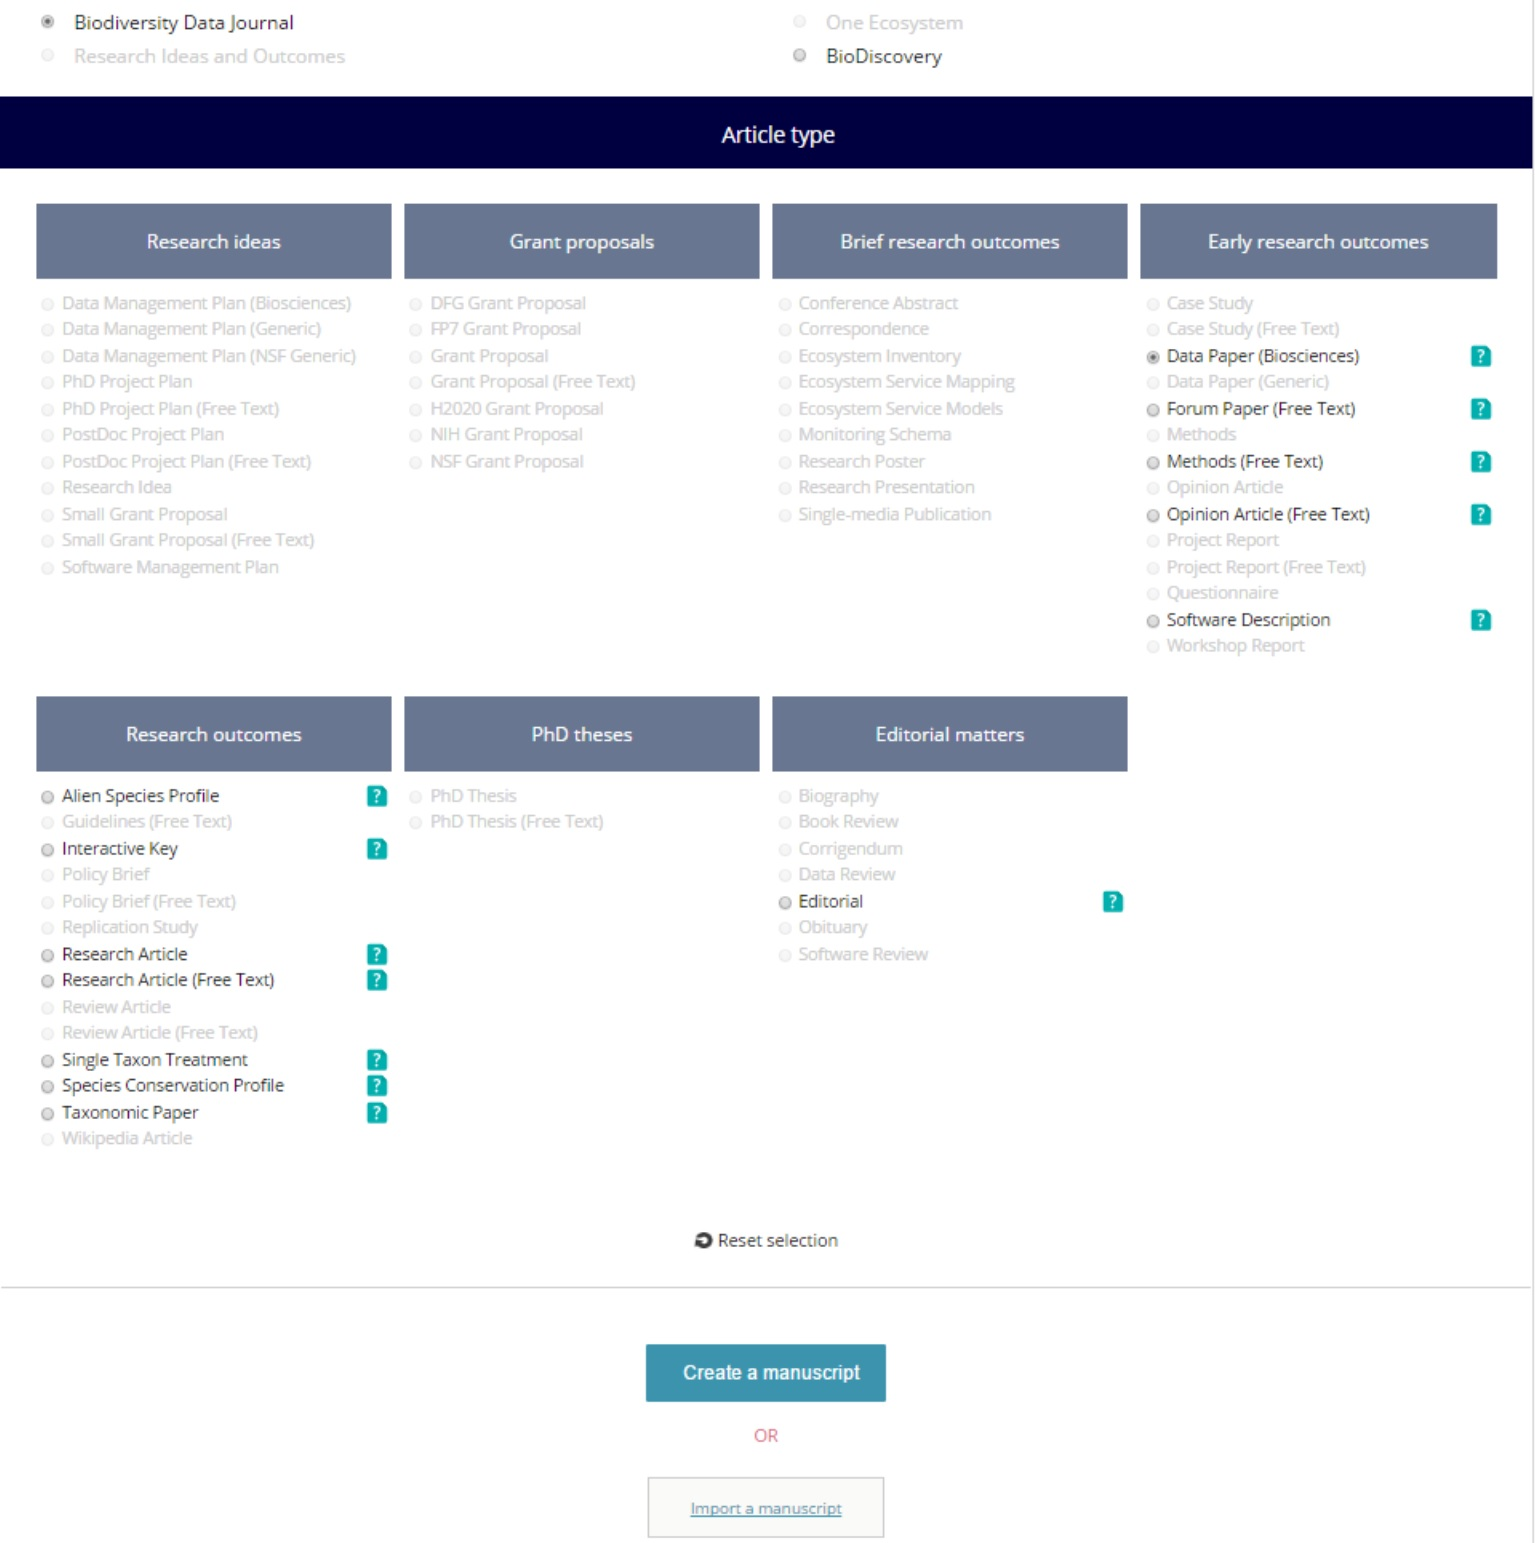
\includegraphics[width=\textwidth]{Figures/journal-selection}
\decoRule
\caption{Selection of the journal and ``Data Paper (Biosciences)'' template in the ARPHA Writing Tool.}
\label{fig:journal-selection}
\end{figure}

\begin{figure}
\centering
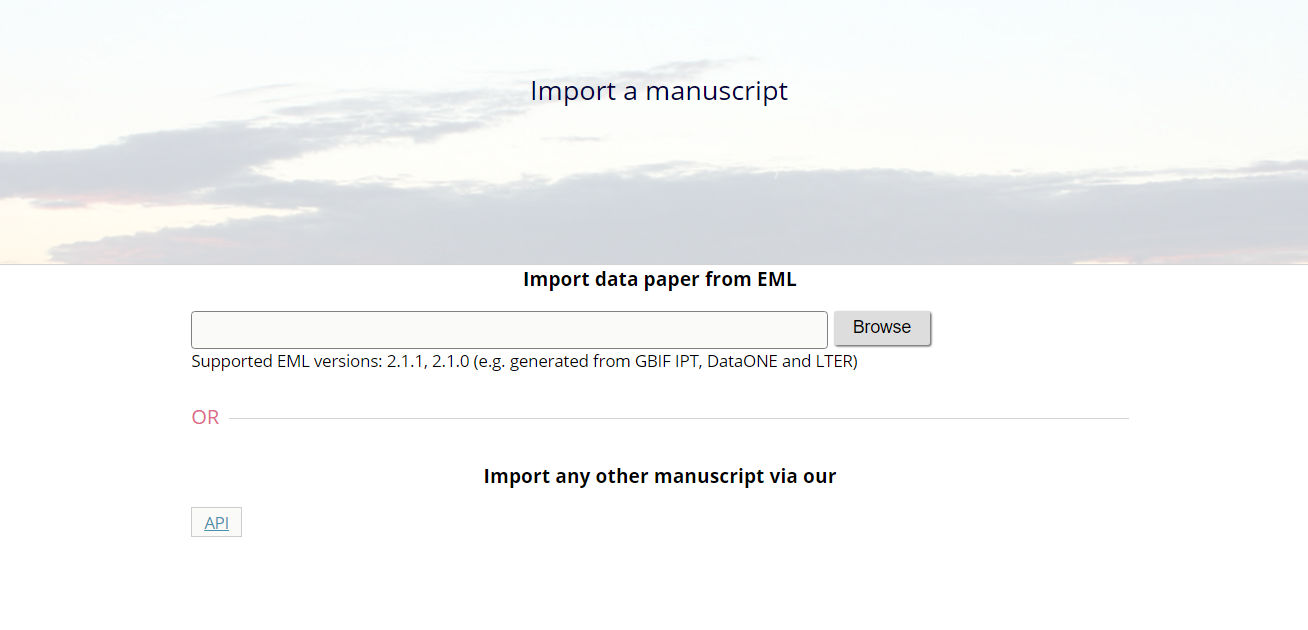
\includegraphics[width=\textwidth]{Figures/user-interface}
\decoRule
\caption{The user interface field for uploading EML files into ARPHA.}
\label{fig:user-interface}
\end{figure}

\subsubsection{Discussion}

I discuss the history of data papers and how our implementation greatly improves the availability of data papers to science practicioners. The two workflows presented generated a lively discussion at the end of the presentation, which is summarized in the Chapter.
\chapter{Резюме на глава 6: Уеб портал}
\label{chapter-webportal}

Под \href{http://openbiodiv.net}{openbiodiv.net} може да се стигне до основния портал, който дава достъп до ресурсите на OpenBiodiv. Този портал е разработен от Pensoft в подкрепа на OpenBiodiv и представя два визуални елемента на потребителя: лентата за търсене и списък с икони на приложения в долната част. Освен това, под \href {http://graph.openbiodiv.net}{{graph.openbiodiv.net}} (също достъпен от иконката SPARQL) може да се достигне работния плот OpenBiodiv за  на SPARQL.

Тези функции на потребителския интерфейс (UI) са предназначени да улеснят трите типа потребители на системата, които предвиждаме:

\begin{enumerate}
\item Основно ниво: използва лентата за търсене.
\item Ниво на специалист: използва приложения.
\item Power user: използва работната плот за SPARQL или R.
\end{enumerate}

\begin{figure}
\centering
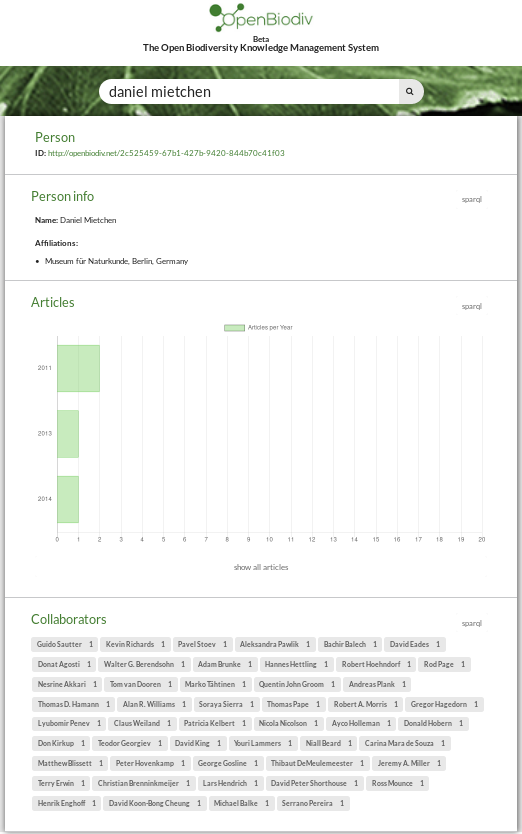
\includegraphics[width=\textwidth]{Figures/basic-level.png}
\decoRule
\caption{Илюстрация на основната употреба на OpenBiodiv за търсене на информация за човек.}
\label{fig:basic-level}
\end{figure}
%\part{Conclusion}
%\label{part:conclusion}


%----------------------------------------------------------------------------------------
%	THESIS CONTENT - APPENDICES
%----------------------------------------------------------------------------------------

\appendix % Cue to tell LaTeX that the following "chapters" are Appendices

% Include the appendices of the thesis as separate files from the Appendices folder
% Uncomment the lines as you write the Appendices

%% Appendix A

\chapter{Frequently Asked Questions} % Main appendix title

\label{AppendixA} % For referencing this appendix elsewhere, use \ref{AppendixA}

\section{How do I change the colors of links?}

The color of links can be changed to your liking using:

{\small\verb!\hypersetup{urlcolor=red}!}, or

{\small\verb!\hypersetup{citecolor=green}!}, or

{\small\verb!\hypersetup{allcolor=blue}!}.

\noindent If you want to completely hide the links, you can use:

{\small\verb!\hypersetup{allcolors=.}!}, or even better: 

{\small\verb!\hypersetup{hidelinks}!}.

\noindent If you want to have obvious links in the PDF but not the printed text, use:

{\small\verb!\hypersetup{colorlinks=false}!}.

%\include{Appendices/AppendixB}
%\include{Appendices/AppendixC}

%----------------------------------------------------------------------------------------
%	BIBLIOGRAPHY
%----------------------------------------------------------------------------------------

\printbibliography[heading=bibintoc]

%----------------------------------------------------------------------------------------

\end{document}  
